%%%%%%%%%%%%%%%%%%%%%%%%%%%%%%%%%%%%%%%%%
% The Legrand Orange Book
% LaTeX Template
% Version 3.0 (January 26, 2022)
%
% This template originates from:
% https://www.LaTeXTemplates.com
%
% Authors:
% Vel (vel@latextemplates.com)
% Mathias Legrand (legrand.mathias@gmail.com)
%
% License:
% CC BY-NC-SA 4.0 (https://creativecommons.org/licenses/by-nc-sa/4.0/)
%
% Compiling this template:
% This template uses biber for its bibliography and makeindex for its index.
% When you first open the template, compile it from the command line with the 
% commands below to make sure your LaTeX distribution is configured correctly:
%
% 1) pdflatex main
% 2) makeindex main.idx -s indexstyle.ist
% 3) biber main
% 4) pdflatex main x 2
%
% After this, when you wish to update the bibliography/index use the appropriate
% command above and make sure to compile with pdflatex several times 
% afterwards to propagate your changes to the document.
%
%%%%%%%%%%%%%%%%%%%%%%%%%%%%%%%%%%%%%%%%%

%----------------------------------------------------------------------------------------
%	PACKAGES AND OTHER DOCUMENT CONFIGURATIONS
%----------------------------------------------------------------------------------------

\documentclass[
	12pt, % Default font size, select one of 10pt, 11pt or 12pt
	fleqn, % Left align equations
	a4paper, % Paper size, use either 'a4paper' for A4 size or 'letterpaper' for US letter size
	oneside, % Uncomment for oneside mode, this doesn't start new chapters and parts on odd pages (adding an empty page if required), this mode is more suitable if the book is to be read on a screen instead of printed
]{LegrandOrangeBook}

% Book information for PDF metadata, remove/comment this block if not required 
\hypersetup{
	pdftitle={Title}, % Title field
	pdfauthor={Author}, % Author field
	pdfsubject={Subject}, % Subject field
	pdfkeywords={Keyword1, Keyword2, ...}, % Keywords
	pdfcreator={LaTeX}, % Content creator field
}


\newsavebox{\fminipagebox}
\NewDocumentEnvironment{fminipage}{m O{\fboxsep}}
 {\\\kern#2\noindent\begin{lrbox}{\fminipagebox}
  \begin{minipage}{#1}\ignorespaces}
 {\end{minipage}\end{lrbox}%
  \makebox[#1]{%
    \kern\dimexpr-\fboxsep-\fboxrule\relax
    \fbox{\usebox{\fminipagebox}}%
    \kern\dimexpr-\fboxsep-\fboxrule\relax
  }\\\kern#2
 }

\addbibresource{sample.bib} % Bibliography file

\definecolor{ocre}{rgb}{0.5, 0.5, 0.5} % Define the color used for highlighting throughout the book
\providecommand{\tightlist}{%
  \setlength{\itemsep}{0pt}\setlength{\parskip}{0pt}}
\chapterimage{orange1.jpg} % Chapter heading image
\chapterspaceabove{6.5cm} % Default whitespace from the top of the page to the chapter title on chapter pages
\chapterspacebelow{6.75cm} % Default amount of vertical whitespace from the top margin to the start of the text on chapter pages

%----------------------------------------------------------------------------------------

\begin{document}

%----------------------------------------------------------------------------------------
%	TITLE PAGE
%----------------------------------------------------------------------------------------

\titlepage % Output the title page
	{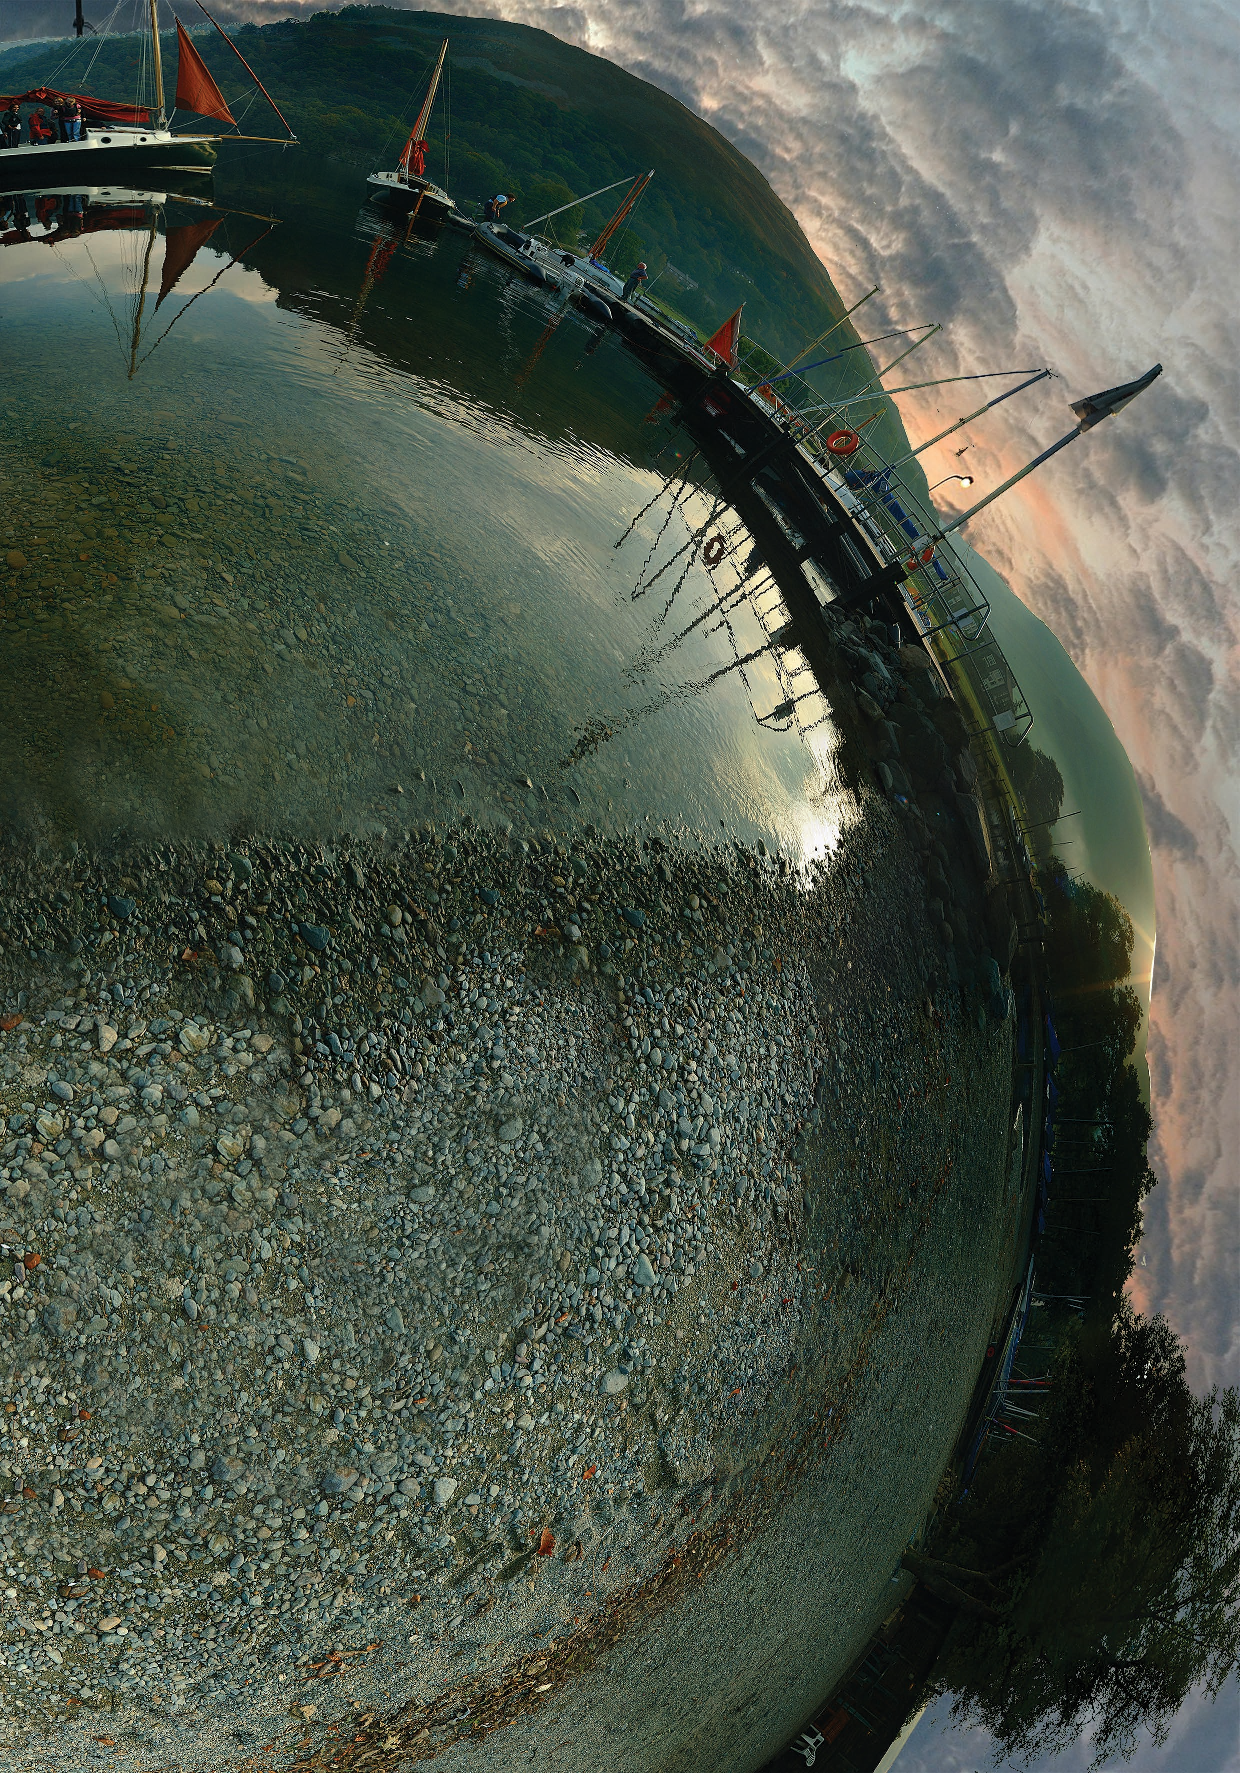
\includegraphics[width=\paperwidth]{background.pdf}} % Code to output the background image, which should be the same dimensions as the paper to fill the page entirely; leave empty for no background image
	{ % Title(s) and author(s)
		\centering\sffamily % Font styling
		{\Huge\bfseries Money in Metaverses\par} % Book title
		\vspace{16pt} % Vertical whitespace
		{\LARGE Bitcoin and stablecoins in global social \\immersive mixed reality systems\par} % Subtitle
		\vspace{24pt} % Vertical whitespace
		{\large \textbf{John O'Hare, Allen Fairchild, and Umran Ali}\par} % Author name
	}

%----------------------------------------------------------------------------------------
%	COPYRIGHT PAGE
%----------------------------------------------------------------------------------------

\thispagestyle{empty} % Suppress headers and footers on this page

~\vfill % Push the text down to the bottom of the page

\noindent \href{https://creativecommons.org/publicdomain/zero/1.0/}{No Copyright}\\ 2022 John O'Hare \& Allen Fairchild \& Umran Ali\\ % Copyright notice

\noindent \textsc{Published by j.ohare@salford.ac.uk for the Cyber Foundry Programme at The University of Salford}\\ % Publisher

\noindent \textsc{\href{https://raw.githubusercontent.com/GMCyberFoundry/Metaverse/main/Paper/metaverseBTC.pdf}{Raw GitHub hyperlink}}\\ % URL

\noindent The person who associated a work with this deed has dedicated the work to the public domain by waiving all of his or her rights to the work worldwide under copyright law, including all related and neighboring rights, to the extent allowed by law.\\
You can copy, modify, distribute and perform the work, even for commercial purposes, all without asking permission. See Other Information below.\\
This license is acceptable for Free Cultural Works.
Other Information\\
In no way are the patent or trademark rights of any person affected by CC0, nor are the rights that other persons may have in the work or in how the work is used, such as publicity or privacy rights.\\
Unless expressly stated otherwise, the person who associated a work with this deed makes no warranties about the work, and disclaims liability for all uses of the work, to the fullest extent permitted by applicable law.\\
When using or citing the work, you should not imply endorsement by the author or the affirmer.\\
\noindent This work was supported by the European Regional Development Fund (ERDF) GM Cyber Foundry Project (15R18P02426)\\

\noindent \textit{First printing, March 2022} % Printing/edition date

%----------------------------------------------------------------------------------------
%	TABLE OF CONTENTS
%----------------------------------------------------------------------------------------

\pagestyle{empty} % Disable headers and footers for the following pages

\tableofcontents % Output the table of contents

\listoffigures % Output the list of figures, comment or remove this command if not required

\listoftables % Output the list of tables, comment or remove this command if not required

\pagestyle{fancy} % Enable default headers and footers again

\cleardoublepage % Start the following content on a new page

%----------------------------------------------------------------------------------------
%	PART
%----------------------------------------------------------------------------------------

\part{State of the art and proposal}

%----------------------------------------------------------------------------------------
%	SECTIONING EXAMPLES CHAPTER
%----------------------------------------------------------------------------------------

\chapterimage{orange2.jpg} % Chapter heading image
\chapterspaceabove{6.75cm} % Whitespace from the top of the page to the chapter title on chapter pages
\chapterspacebelow{7.25cm} % Amount of vertical whitespace from the top margin to the start of the text on chapter pages

%------------------------------------------------

\section{Conflict of interest statements}
The authors may own small numbers of the various tokens referenced in the text for experimentation and/or investment purposes. At this time that is only sufficient Ethereum to operate a Web3 wallet, and Bitcoin locked on the Lightning network. No NFTs are owned at this time. There are no financial stakes in the development of any of these ecosystems.
\chapter{Introduction}
\section{Overview}

In the last couple of years the Greater Manchester Cyber Foundry has been collaborating with small to medium sized enterprises, responding to their questions about emerging trends. We were asked about exciting new developments in the transmission of value, and trust in Metaverses. The problem is that each of these topics alone are enormously complex, and the intersections seem to be more so. We have been researching the current state-of-the-art, and the emerging consensus narrative, to try to figure out how the collision of these technologies might serve SMEs. \par
Because we’re the GM Cyber Foundry, we started out with security best practices in mind. How can we enable small and especially developing companies, to have a foot in the door on a global stage, without their cybersecurity costs spiralling? Fortunately, we discovered a wealth of carefully crafted open source tools which can support this exploration. We have tried to assemble them cogently, to deliver a kit for experimentation to curious technically minded SMEs, and we have applied our own security knowledge on top of an already top class set of tools. It’s certainly not production ready, but it's good enough to commit small amounts of money into, for experimentation purposes.\par
Whilst researching, it seemed that every door we opened was full of interesting and useful treats. What was supposed to be a short technical paper quickly became a 150-page book, and a deployable virtual machine stack, with a dozen different open source components in it. \par
To that end, this book supports the virtual lab, which supports anyone who thinks this material might be useful. In the following sections you’ll read a precis of the sections of the book, which will hopefully give an insight into what ``this stuff'' is. Then you can decide to download the book and the lab how to guide. All of it is open source, all of it can be contributed to on GitHub, all of it will be developed forward, and none of it is really finished yet.
Section 1  attempts to overview what the book is about, which is value transmission, with distributed trust, in global social mixed reality systems. \par
Next is a summary of Web3, as it stands right now. Web3 is a complex term and it’s cropping up far more in the technical press so we wanted to cover off what it might mean, but honestly, it’s still pretty confusing. There are a bunch of legacy explanations which are Web3.0, that are withering on the vine. Then there’s the new VC funded, super hyped and potentially useless Web3 incarnations, which again cover a slew of intersecting technologies. This doesn’t mean there’s nothing to see here. The astonishing amount of money and developer talent, and the clear market hunger for things like NFTs (non-fungible tokens) suggest that there’s a future for Web3, it’s just really unclear what the value could be for our curious SME.\par
In the next section we took a look at blockchain, which is very intersectional with Web3. Even on its own this is a very complex emergent set of disciplines. \par
The blockchain section was especially interesting to research. It turns out there’s a LOT of ways to get this technology wrong. Even very appealing options on paper, turn out to have very shaky foundations. There are really valuable things here, but given the complexity, and the size of that chapter, we decided to focus down on the most promising of the technology stacks, which interestingly turned out to be the original; the Bitcoin network.\par
Even Bitcoin isn’t just Bitcoin anymore. It’s a swarm of open source tools which can (in theory) accomplish a great many things. These newer, ancillary elements to Bitcoin, are emergent right now. Some of the won’t be around until later in the year and it’s questionable whether they will even work out. With that said there’s already enough here for us to cherry pick some useful components and start to map those forward into our metaverse proposal.\par
In looking around at the available options, it seems possible that the features which are important to Web3 in section 1, can also potentially arise from the Bitcoin technology that we settled on in section 2. This was somewhat unexpected, so we started mapping that over too.\par
The next section is about Money. In expanding our research on Bitcoin, we found that it’s impossible to think about the tech without opening up a whole other line of questions about money itself. This is fine because we set out to look at global value transfer for business. It’s not a trivial subject though, and this section tries to overview why value and Bitcoin are so enmeshed then what other options there might be in the end (because Bitcoin has kicked off a whole slew of global adoption outside of itself) and finally what we can do pragmatically, both now, and in the coming year or two.\par
The distributed identity management, and trust section follows. It’s not an easy section to write about, because there’s a lot of research, it’s not our field, and finding the value to SMEs has actually been very difficult. This section is likely to be overhauled a few times in the coming months as we settle on technologies that we believe are simple and secure enough.\par
In section 7 we take another look at NFTs. It’s impossible to ignore this stuff now. It’s fundamentally a bit broken, but there are likely some use cases, and the money and development attention it’s getting are incredible. We try to navigate our hypothetical SME through this as best we can. It’s not that we didn’t understand it completely, just that the tech moves so very fast that it’s impossible to even describe what’s going on accurately at any given point. We’re actually pretty excited about future versions of this technology, based around Bitcoin, because that allows us to keep just one value stack in the  lab. We’ve mapped that forward into the open source tools that we recommend. This very much ended up looking like our priors; our cyber security values, and our wish to build toward a simpler product using only Bitcoin. To that end we asked another author, with much more of a foot in the content creation world, to collaborate with us on this chapter. This will benefit from smoother integration over the coming months.\par
Chapter 8 is a big one for us as it’s our research area prior to opening up the Bitcoin box(es).\par Metaverse, or at least one of the current definitions of metaverse, is just social interaction in mixed reality (VR/AR/XR!). We’ve been studying that for decades, so this section is more academic and tried to boil down what we think is most important to map forward into the lab. The choices we make here guided us toward the selection of free and open source metaverse software, which we selected from a bunch that we reviewed. You can make your own choices and gain insight from the systems we looked at.\par
We also take a look at the other definitions of metaverses which are doing the rounds on the web, try to unpick which is which, and what they are for, then we attempt to weave back together the best of both. This ends up looking a bit like the Venn at the top, where we have transmission of provable identity, non-fungible tokens bearing value or data, distributed files, actual money (including micropayments) and a social layer based on our best knowledge about mixed reality.\par
Past this stage in the book we get into the murky and half developed tail end where we’re interfacing with our design choices, and the stack which can be deployed into the cloud.



\section{Introduction}
This document presents a high level view of technologies and their potential within the emergent Web3 and metaverse narrative, focusing around the transmission of value within and across such global networks, with a further focus on the Bitcoin monetary network. It was written to organise the thoughts of the authors, who were unfamiliar with Bitcoin technologies until recently.\par
As adoption of these technologies increases it will be necessary for people, and AI actors, to pass economic value between themselves. These `goods and services' interactions, within the virtual social spaces should be underpinned by a trust system, which scales globally and presents low friction. Current secure international payment rails are poorly suited to such interactions; indeed it is likely with legacy systems, that parties would be forced to leave the metaverse application, and instead navigate their banking applications to exchange value with overseas entities in a secure fashion. This might conceivably take several days.\par 
Fortunately, the whole landscape of money and \href{https://www.omfif.org/futureofpayments2021/}{value transfer is changing}. Huge global financial players are entering the space. HSBC have \href{https://sandboxgame.medium.com/hsbc-to-become-the-first-global-financial-services-provider-to-enter-the-sandbox-c066e4f48163}{just bought} metaverse `land' in The Sandbox, JP Morgan have \href{https://www.forbes.com/sites/ronshevlin/2022/02/16/jpmorgan-opens-a-bank-branch-in-the-metaverse-but-its-not-for-what-you-think-its-for/?sh=2fbd1e90158d}{opened a `lounge'} in another. The worlds largest hedge fund Bridgewater is stepping into \href{https://uk.finance.yahoo.com/news/bitcoin-latest-price-crypto-ray-dalio-bridgewater-investment-fund-ethereum-094946686.html}{acquisition of digital assets}, and the world's largest pension fund manager Blackrock is adding these asset to their management engine (which manages tens of trillions of dollars). Fidelity asset management are about to add \href{https://www.wsj.com/articles/fidelity-to-allow-retirement-savers-to-put-bitcoin-in-401-k-accounts-11650945661}{Bitcoin to their pension plans} and are offering a \href{}{dedicated metaverse tradable fund}, while \href{https://www.citivelocity.com/citigps/metaverse-and-money/}{Citigroup have a minisite} dedicated to ``Metaverse and Money''. The front page of Goldman Sachs recently says it all (Figure \ref{fig:goldmanFront}).\par
\begin{figure}[ht]\centering % Using \begin{figure*} makes the figure take up the entire width of the page
	\includegraphics[width=0.5\linewidth]{goldmanFront}
	\caption{The landing page of global\\financial giant Goldman Sachs shows the hype.}
	\label{fig:goldmanFront}
\end{figure}
Of their recent investments KPMG global said: \textit{``We've invested in a strong cryptoassets practice and we will continue to enhance and build on our capabilities across Decentralized Finance (DeFi), Non-Fungible Tokens (NFTs) and the Metaverse, to name a few''}.\par
It's possible that for such organisations it makes better business sense to take a punt on hype bubbles like this, than to do a proper due diligence with a team of internal staff who understand their business. These endorsements should be taken with a large pinch of salt. As \href{https://newsletter.fintechtakes.com/p/metaverse-branches?s=r}{Alex Johnson says}: \textit{``At some point in the future, it’s possible that the digital worlds being built today will have aggregated sufficient user attention and engagement that financial services companies will need to invest in the metaverse as an acquisition and customer service channel. But we’re not there yet. Until the metaverse is a little less empty, resist the temptation to colonize it with branches and billboards.''}\par
Meanwhile, Meta (ex Facebook) are launching their own \href{https://archive.ph/coyp2}{META Web3 and metaverse} token (after abandoning Libre, their global cryptocurrency), and \href{https://www.cnbc.com/2022/05/06/googles-cloud-group-forms-web3-product-and-engineering-team.html}{Google} have \href{https://blog.youtube/inside-youtube/innovations-for-2022-at-youtube/}{recently blogged}: \textit{``Web3 also opens up new opportunities for creators. We believe new technologies like blockchain and NFTs can allow creators to build deeper relationships with their fans. Together, they'll be able to collaborate on new projects and make money in ways not previously possible. For example, giving a verifiable way for fans to own unique videos, photos, art, and even experiences from their favourite creators could be a compelling prospect for creators and their audiences. There's a lot to consider in making sure we approach these new technologies responsibly, but we think there's incredible potential as well. Finally, we couldn't have a piece about innovation without touching on the metaverse! We're thinking big about how to make viewing more immersive. ''}\par
It's already the case that the recent bubble of \href{https://www.forbes.com/sites/paultassi/2022/03/10/interest-in-nfts-and-the-metaverse-is-falling-fast/?}{hype is dwindling}, but the enormous investment into teams and startups will potentially bear fruit in the next couple of years, and this perhaps has implications for small and medium-sized enterprises (SMEs). \par
In the UK the government has stated it's ambition to be a \href{https://www.gov.uk/government/news/government-sets-out-plan-to-make-uk-a-global-cryptoasset-technology-hub}{global cryptoasset technology hub}, and announced plans for the Royal Mint to issue a (novelty) NFT. Like the assertion by major global businesses it is too early to tell how `sticky' these claims are.\par
With all this attention it seems timely to explore the potential of recent technologies, which can address metaverse interactions in \textit{business to business} (B2B), \textit{business to customer} (B2C), and the newer C2C (social commerce; \textit{creator to consumer, customer to customer, consumer to consumer\cite{jones2008trust})}. Figure \ref{fig:landscapevenn} demonstrates how some of these domains intersect.\par
This book seeks to overview and explain the available open source technologies. It supports an open source \href{https://github.com/GMCyberFoundry/Metaverse}{github repository} which enables SMEs to access these emergent platforms and ecosystems. It aims to build toward a minimum viable product for trust minimised transfer of value within a social immersive space.\par
Referencing is in two styles; academic works and books are numeric, while opinion pieces, gray statistics, and pertinent news articles are hyperlinked from the text. This hybrid style yields about twice the citation density of a normal PhD thesis, which is a lot. For this reason the normal blue hyperlink colour was eschewed in favour of a more aesthetic ``gray''. There is also a version of the PDF which complies with accessibility best practice if this is a problem.  \par 
\subsection{Notes on progress}
\textbf{This version of the book is ``minimally complete''. The real interesting work of combining the primitives into a new direction for integration of Bitcoin and VR is just beginning. We are now inviting the wider community to submit pull requests into github as contributors. It's been a useful document creation process to form our thoughts, and it's enough to bring a reader up to ``the state of the art'' if all of the thousand  links and papers are considered. It's an open ended project though.}\

\begin{figure*}[ht]\centering % Using \begin{figure*} makes the figure take up the entire width of the page
	\includegraphics[width=\linewidth]{landscapevenn}
	\caption{Web 3, Metaverse, and Bitcoin are inter-sectional technologies.}
	\label{fig:landscapevenn}
\end{figure*}
\chapter{Web3 / decentralised web}
Web3 is a rapidly evolving set of technologies and specifications which are drifting further from their origin. Decentralised web is perhaps a more useful name, but focus in this section will be on the evolution of the popularised term Web3. 
\section{Semantic web}
The ``semantic web'' definition of Web3.0 has been somewhat overhauled by other innovations in decentralised internet technologies, now evolving toward the slightly different Web3 moniker. Tim Berners Lee (of WWW fame) first mentioned the semantic web in 1999 \cite{semanticWeb}.\\
``I have a dream for the Web [in which computers] become capable of analyzing all the data on the Web – the content, links, and transactions between people and computers. A "Semantic Web", which makes this possible, has yet to emerge, but when it does, the day-to-day mechanisms of trade, bureaucracy and our daily lives will be handled by machines talking to machines. The "intelligent agents" people have touted for ages will finally materialize.''\\
Attention developed around three core themes, ubiquitous availability and searchability of data, intelligent search assistants, and highly available end points such as phones, and `internet of things' devices. This is certainly manifesting in home devices, but few people think of this as a Web3 revolution. The framework can be seen in Figure \ref{fig:semanticWebStack}.\\
\begin{figure}
  \centering
    \includegraphics[width=\linewidth]{semanticWebStack}
  \caption{\href{https://en.wikipedia.org/wiki/Semantic_Web_Stack}{Semantic Web Stack} [CC0 image]}
  \label{fig:semanticWebStack}
\end{figure}
Since ratification of the standards by the \href{https://www.w3.org/standards/semanticweb/}{World Wide Web (W3C) consortium} it seems that their imperative toward decentralisation has become lost. Instead it can be seen that Facebook, Amazon, Google, and Apple have a harmful oligopoly on users data \cite{costigan2018world}. This is as odds with Berners-Lee's vision. \\
It is worth taking a look at his software implementation called \href{https://solidproject.org}{Solid}, which is far more mindful of the sovereignty of user data.\\
``Solid is an exciting new project led by Prof. Tim Berners-Lee, inventor of the World Wide Web, taking place at MIT. The project aims to radically change the way Web applications work today, resulting in true data ownership as well as improved privacy. Solid (derived from "social linked data") is a proposed set of conventions and tools for building decentralized social applications based on Linked Data principles. Solid is modular and extensible and it relies as much as possible on existing W3C standards and protocols.'' \\
Excitement around this kind of differentiated trust model, hinted at in ubiquitous availability of data (and implemented explicitly in Solid), has led to exploration of different paths by cyptographers, and this will be described later.\\
\section{Spatial web}
``The Spatial Web'', a blurring of the boundaries between digital and geospatialised physical objects, seems to have developed from the strands in the original W3C scope around devices in the real world. It has been concentrating around AR and VR, but is being marketed and amplified with the same references to availability of data (See Figure \ref{fig:deloitteSpatial} from a Deloitte accounting report). This too is finding little traction in practice, though obviously the component technologies continue to enjoy rapid development. Nontheless, this interpretation of Web3 becomes valuable when examining Metaverse later.\\
\begin{figure}
  \centering
    \includegraphics[width=\linewidth]{deloitteweb3}
  \caption{\href{https://www2.deloitte.com/us/en/insights/topics/digital-transformation/web-3-0-technologies-in-business.html}{Deloitte Spatial Web Overview} Reused with permission.}
  \label{fig:deloitteSpatial}
\end{figure}
\section{Webs of trust}
More recently Web3 is \href{https://trends.google.com/trends/explore?date=all&q=web3}{being touted} as a way to connect content creators directly to content consumers, without centralised companies acting as gatekeepers of the data. It implies that all users have a cryptographic key management system, to which they attach metadata, that they make requirements of peers with whom they communicate, and that they maintain trust `scores' with peers.\\
It seems likely that this new model is less driven by a market need, and more by the high availability of tools which allow this to happen (the ecosystems described later). Add to this a social response to the \href{https://finance.yahoo.com/news/meta-facebook-worst-company-of-the-year-yahoo-finance-165345819.html}{collapse in trust of companies such as Facebook} (Figure \ref{fig:trustbarometer}), a wish by consumers to pass more of the economic incentive to content creators, without the `rent seeking' layer afforded by businesses, and a healthy dose of mania driven market speculation. 

\begin{figure}
  \centering
    \includegraphics[width=\linewidth]{c-a-e}
  \caption{\href{https://www.edelman.com/trust/2020-trust-barometer}{Edelman 2020 trust barometer} [rights requested]}
  \label{fig:trustbarometer}
\end{figure}
\section{Emerging consensus}
It's possible to frame Web3 as  a hugely complex and inefficient digital rights management system (DRM). DRM is something that users of the internet are increasingly familiar and comfortable with. It's somewhat debatable whether decentralising this is worthwhile. The thesis of the developers of the technology seems to be that without it, control of `value' will accrete over time, to one or more hegemonic controlling entities. It's a strong argument, but there is a \href{https://moxie.org/2022/01/07/web3-first-impressions.html}{substantial counter argument} emerging that users just don't want this stuff. The nervousness of legislators in the USA to the attempt by Facebook/Meta to enter this peer to peer value transmission space is telling in terms of the perception of who is driving Web3.\\
At the end of 2021 and beginning of 2022 there is much furore on the internet over what Web3 might be, and who it `serves'. 
Enthusiasts feel that products such as \href{https://blog.spruceid.com/sign-in-with-ethereum-is-a-game-changer-part-1/}{Sign-In with Ethereum} (EIP-4361) will give users choice over their data sovereignty, and a meme to this effect is seen in Figure \ref{fig:web1web2web3}. In practice though users are expecting to use badly written, buggy, economically vulnerable `crypto' wallets to log into websites. It doesn't seem to make much sense yet on the face of it. This will be explored further in the distributed identity section. \\
\begin{figure}
  \centering
   \includegraphics[width=\linewidth]{web1web2web3}
 \caption{A meme showing differing approached to logging in on a website.}
 \label{fig:web1web2web3}
\end{figure}
The current hype cycle is ignoring the legacy definitions described above and instead focusing almost exclusively on Ethereum based peer to peer projects (more on these later). It can be seen that the description is somewhat in the eye of the beholder.\\
This new hyped push for Web3 is being driven by enormous venture capital investment. A16Z are a \href{https://a16z.com/2022/01/07/9b-to-build-the-future/}{major player} in this new landscape and have released their \href{https://a16z.com/2022/01/07/how-to-build-a-better-internet-10-principles-for-world-leaders-shaping-the-future-of-web3/}{ten principles} for emergent Web3. 
\begin{itemize}
\item Establish a clear vision to foster decentralized digital infrastructure
\item Embrace multi-stakeholder approaches to governance and regulation
\item Create targeted, risk-calibrated oversight regimes for different web3 activities
\item Foster innovation with composability, open source code, and the power of open communities
\item Broaden access to the economic benefits of the innovation economy
\item Unlock the potential of DAOs
\item Deploy web3 to further sustainability goals
\item Embrace the role of well-regulated stablecoins in financial inclusion and innovation
\item Collaborate with other nations to harmonize standards and regulatory frameworks
\item Provide clear, fair tax rules for the reporting of digital assets, and leverage technical solutions for tax compliance
\end{itemize}
Many of the mentioned components here will be described later in the book. This list seems targeted toward the coming regulatory landscape, and could be considered at odds with the original tenants of an organically emergent, decentralised internet.\\
Dante Disparte, chief strategy officer of Circle, said in testimony to US senate hearing; that Web 1 was `read', Web 2 was `read write', and that Web 3 will `read write own'. The important takeaway here is not so much this oft quoted elevator pitch for Web3, but the fact that legislative bodies now consider this technology a force which they need to be aware of and \href{https://a16z.com/2021/12/17/prediction-for-the-new-year-a-web3-midterm/}{potentially contend with}. The suggestion is that this is happening regardless of a decent use case or definition.\\
It's a complex evolving narrative, and clearly contradictions are common. Into this confusion this book advances a narrow take, and toolset, which might extract some value from the technologies, while maintaining a low barrier to entry.\\ 

\section{Example applications}
\subsection{Podcasting2.0}
\href{https://medium.com/@everywheretrip/an-introduction-to-podcasting-2-0-3c4f61ea17f4}{Podcasting 2.0} leverages RSS (the original dissemination system for podcasts) and the Bitcoin Lightning network, to enable so-called `value for value' broadcasting. Subscribers use one of a variety of apps to stream microtransactions of Bitcoin directly to the content creators as they listen to the podcast. No intermediate business takes a cut. Some variation on this model exists, such as John Carvalho's crowd funded podcast ``The Biz'' which progressively unlocks more minutes for everyone based on \href{https://thebiz.pro/about#crowdwall}{crowd funded donations}.
\subsection{Crowd funding}
At time of writing a \href{https://www.constitutiondao.com/}{crowd funding initiative} based around a digital decentralised construct called a DAO (explained later in detail) \href{https://www.coindesk.com/business/2021/12/06/daos-and-the-next-crowdfunding-gold-rush/}{managed to raise \$46 million dollars to bid for a copy of the US constitution} at Southerbys auction house. The attempt narrowly failed, but the press \href{https://www.coindesk.com/business/2021/12/09/what-kickstarter-going-decentralized-means-for-web-3/}{heralded this new era of ``Web3'' economic might}. This model might be the only use for DAOs and is likely just a way to avoid regulatory scrutiny. There is more detail on DAOs later.
\subsection{Distributed exchanges}
There are dozens of decentralised exchanges deployed on various blockchains. These platforms allow users to trade back and forth between various tokens (including `normal money' stablecoins), and charge a fee for doing so. They operate within the logic of the smart contracts, within the distributed blockchains. This makes them extremely hard to ban, and as a result they operate in a legal gray area. At the extreme end of this is ``distributed apps'' (dApps) and ``Decentralised Finance'' (DeFi) which allows users access to complex financial instruments without legal or privacy constraints. DeFi will be touched on briefly later.\\
This is a huge area, and of only limited interest to the topics expanded in this book. It's perhaps worth noting \href{https://bitcoin-dex.net/about/index.html}{BitcoinDEX}, which runs in javascript in a web browser. It is effectively uncensorable, \href{https://bitcoin-dex.net/tokens.js}{auditable by the user}, and has no counter party risk since it operates entirely in the Bitcoin network. It is clearly an early prototype, but manages this complex feature without the more expressive logic of more `modern' public blockchains.
\subsection{NFT marketplaces}
NFT markets are far more centralised services which match `owners' of digital assets with potential buyers. The concept is a staple of the more recent interpretation of Web3, even though in practice these seem to be centralised concerns. \href{https://opensea.io/}{Opensea} claims to be the largest decentralised NFT marketplace, but they have the ability to \href{https://thedefiant.io/sad-frogs-delisted-opensea/}{remove listings} in response to legal challenges. This seems to fly in the face of Web3 principles. NFTs are currently a \href{https://tante.cc/2021/12/17/the-third-web/}{deeply flawed} technology but seem likely to persist and will be covered later.
\subsection{Slashtags / Hypercore}
Slashtags is a web of trust model decentralised peer to peer model which assigns metadata and trust scores to `any' data and connection, with a security model rooted in the Bitcoin cryptographic `keys' but crucially not the bitcoin network. This makes it interoperable with bitcoin but not reliant upon it. In principle this allows users to build complex networks of inherited trust bi-directionally with their networks over time. Every connection to a peer can be a new schema, with individual metadada managed by the user. It is new and has low adoption at this time. The user controls the source of the data and can allow them to be used by centralised services. This flips the authentication and data management paradigm of Web2 around, putting the user in charge of their data. This is a familiar concept to the DID/SSI communities (described later) but with significant investment. As Slashtags use keys as endpoints they act as a web of naming and routing, bypassing the existing web infrastructure of DNS. It is likely very complex to use in practice and will be revisited later. It is being paired with the \href{https://hypercore-protocol.org/}{Hypercore protocol} for peer to peer data sharing, more specifically the `hole punching' capability of the hypercore system which ensures connections through firewalls\cite{ford2005peer}. The first application by the affiliated Hyperdivision team is an open source pear to peer live video streaming app called \href{https://dazaar.com/}{Dazaar}. Once again, it's not clear yet who wants or needs this bit-torrent style service. 
\subsection{Distributed DNS applications} 
There are many perceived problems with having centralised authorities for overseeing the database which translates between human readable internet names and the underlying machine readable address notation. The databases which manage this globally are already somewhat distributed, and this distributed trust model is managed through a cryptographic chain of trust called DNSSEC which is capped by a somewhat \href{https://www.iana.org/dnssec/ceremonies}{bizarre key ceremony}. The authority around naming is centralised in ICANN. There has been talk for many years about `properly' distributing this database using decentralised/blockchain technologies\cite{karaarslan2018blockchain}. The nature of this problem means that it either moves from control by ICANN, or it does not, and so far it has not, but there are many attempted and somewhat mature attempts at this difficult problem. Of these \href{https://www.namecoin.org/}{Namecoin} is the most prominent, and is a fork of Bitcoin. The ubiquity of Bitcoin in such systems is perhaps becoming apparent.
\subsection{Impervious browser}
It might be that the future of Web3 comes in the guise of integrated suites such as the proposed \href{https://newsletter.impervious.ai/impervious-browser-functionality-overview/}{Impervious web browser}. They say that ``without centralized intermediaries'' it features:
\begin{itemize}
\item    Zoom, without Zoom.
\item    Google Docs, without Google.
\item    Medium, without Medium.
\item    WhatsApp, without WhatsApp.
\item    Payments, without banks.
\item   Identity, without the state.
\end{itemize}
This is obviously leading marketing hype, but what they're talking about here is an integration of the components mentioned in this book. If they can get critical mass around this browser then perhaps the Web3 market can be kickstarted.
\section{The common thread}
One feature which persists throughout all of these interpretations of Web3 is the need for decentralised trust. If there is to be no central controlling party(s) as in the Web 2 model then nothing can happen without a cryptographically secure underpinning, which favours no party beyond the terms of their collectively agreed rights and privileges. From this base layer we also get the potential for secure and trust minimised identity management. This nascent field of distributed identity management is explained later. From distributed trust models we can see `trustless' transmission of economic value. The ability to send value from one person to another person or service without a third party. This whole area is `Crypto', which is increasingly seeping into the human consciousness, and saw an astonishing \$13B of \href{https://docsend.com/view/nrvsuae85a4dx3jz}{capital investment in 2021} alone. At time of writing the industry is a \href{https://www.coingecko.com/en}{over 2 trillion} dollar market. According to \href{https://www.coindesk.com/podcasts/the-breakdown-with-nlw/yesterdays-hearing-was-cryptos-most-positive-interaction-with-the-us-government-ever/}{Nathaniel Whittemore}, a journalist for Coindesk, ``The Web3 moniker positions this industry in opposition to big tech''. In practice it seems that this is just another avenue for existing players to experiment with new \href{https://www.cigionline.org/articles/amid-the-hype-over-web3-informed-skepticism-is-critical/}{models of control}, and is \href{https://web3isgoinggreat.com/}{rife with scams}.\\
Of their 2022 \href{https://research.ark-invest.com/thank-you-big-ideas-2022?submissionGuid=0937b1ae-9e11-4b46-ae03-6cd8d2f8301b}{`Big Ideas' report}, ARK investment LLC (who manage \$50B tech investment) \href{https://www.ark-bigideas.com/2022/en/pages/download}{said the following} (Figure \ref{fig:ARKWeb3}), which connects some of the dots already mentioned, and leads us into the next section which is Blockchain and Bitcoin:\\
\textit{``While many (with heavily vested interests) want to define all things blockchain as web3 we believe that web3 is best understood as just 1 of 3 revolutions that the innovation of bitcoin has catalyzed.
\begin{itemize}
\item The Money Revolution
\item The Financial Revolution
\item The Internet Revolution''
\end{itemize}}
\begin{figure}
  \centering
    \includegraphics[width=\linewidth]{Web3ARK}
  \caption{\href{https://twitter.com/wintonARK/status/1486143239753060353}{ARK slide on Web3.} Rights requested}
  \label{fig:ARKWeb3}
\end{figure}
All these new `crypto' technologies are bound tightly together, but there is currently very little meaningful value to be seen. The rest of this book will focus on the money revolution element of this shift in internet technologies, and attempt to build a case for it's use in metaverse applications.
\section{Risks}

\chapter{DLT, Blockchain, and Bitcoin}
Distributed ledger technology (DLT) is a data structure distributed across multiple managing stakeholders. A subset of DLT is blockchain, which is a less efficient, immutable data structure with a slightly different trust model. Rauchs et al. of the Cambridge Centre for Alternative Finance provide a detailed taxonomy and conceptual framework \cite{rauchs2018distributed}. It can be seen in their paper that the definitions are somewhat unclear in literature.\par
DLT, and especially blockchain, are rapidly gaining ground in the public imagination, within financial technology companies (FinTech), and in the broader corporate world. \par
The technology and the global legislative response are somewhat immature, and misapplications of both technologies are commonplace. \par
Distributed trust models emerged from cryptography research in the 1970s when Merkle, Diffie, and Hellman at Stanford worked out how to \href{https://medium.com/swlh/understanding-ec-diffie-hellman-9c07be338d4a}{send messages online} without a trusted third party \cite{diffie1976new,merkle1978secure}.\par
Soon after the 1980s saw the emergence of the cypherpunk activist movement, as a reaction to the emerging surveillance state \cite{burnham1983rise, chaum1985security}. These early computer scientists in the USA saw the intersectionality between information, computation, economics, and personal freedom \cite{lavoie1990prefatory}. Online discussion in the early nineties foresaw the emergence of trans-national digital markets, what would become the WWW \cite{salinCosts, cypherPunkMailList}. The issues of privacy %(https://nakamotoinstitute.org/static/docs/cypherpunk-manifesto.txt) 
 and the exchange of digital value (digital / ecash) %(https://www.wired.com/1994/12/emoney/  https://www.cs.ru.nl/~jhh/pub/secsem/chaum1985bigbrother.pdf) 
 were of foremost importance within these discussions %(https://www.wired.com/1994/12/emoney/), 
 and while privacy was within reach thanks to \href{https://www.openpgp.org/about/history/}{``public/private key pairs''}, 
 ecash proved to be a more difficult problem. \par
Adam Back's 1997 `hashcash' \cite{back2002hashcash} paved the way for later work by introducing the concept of `proof of work'. This was built upon by Dai \cite{dai1998b}, Szabo \cite{szabo1997formalizing}, Finney \cite{callas1998openpgp}, and Nakamoto amongst others. In all it took 16 years of collaboration on the mailing lists to attack the problem of trust-minimised, distributed, digital cash. The culmination of these attempts was Bitcoin \cite{Nakamoto2008}. This is illustrated by Dan Held in Figure \ref{fig:prehistory}. This is now a wider ecosystem of technologies. 

\begin{figure}
  \centering
    \includegraphics[width=\linewidth]{prehistory}
  \caption{Dan Held: \href{https://www.danheld.com/blog/2019/1/6/planting-bitcoinsoil-34}{Bitcoin prehistory} used with permission.}
  \label{fig:prehistory}
\end{figure}

There is enormous complexity and scope, as seen in Figure \ref{fig:venn}, and yet genuinely useful products are elusive.
\begin{figure*}[ht]\centering % Using \begin{figure*} makes the figure take up the entire width of the page
	\includegraphics[width=\linewidth]{venn}
	\caption{\href{https://unchained.com/blog/blockchain-spectrum/}{Intersecting disciplines}. Reused with permission \href{https://unchained.com/}{Dhruv Bansal}}
	\label{fig:venn}
\end{figure*}
It is surprisingly hard to pin down a simple explanation for the features which define a blockchain. These ``key takeaway'' \href{https://www.investopedia.com/terms/b/blockchain.asp}{from Investopedia} are a neat summary however.\par
\begin{itemize} \item Blockchain is a specific type of database. \item It differs from a typical database in the way it stores information; blockchains store data in blocks that are then chained together. \item As new data comes in it is entered into a fresh block. Once the block is \href{https://bits.monospace.live/}{filled with data} it is chained onto the previous block, which makes the data chained together in chronological order. \item Different types of information can be stored on a blockchain but the most common use so far has been as a ledger for transactions. \item In Bitcoin’s case, blockchain is used in a decentralized way so that no single person or group has control—rather, all users collectively retain control. \item Decentralized blockchains are ``append only''. In effect this means that the data entered becomes irreversible over time. For Bitcoin, this means that simple economic transactions are permanently recorded and viewable to anyone. \end{itemize}
In principle blockchains provide a differentiated trust model. With a properly distributed system a blockchain can be considered ``trust-minimised''. This is important for some, but not all people. \par
It can also be argued that the whole concept of distributed cryptographic blockchains is somewhat strained, as the vast majority of the technology offerings are not properly distributed, and ``there are many scenarios where traditional databases should be used instead''\cite{casino2019systematic}.\par
The proponents of blockchains argue, that in an era when data breaches and corporate financial insolvency intersect with a collapse in trust of institutions, it is perhaps useful to have an alternative model for storage of data, and value. Thanks to a natural fit with strong encryption, and innate resistance to censorship by external parties, these systems do lend themselves well to `borderless' applications, and are somewhat resistant to global regulation (for good or ill). Finally, a host of well engineered open source code repositories makes the cost of adoption relatively low.\par
Within DLT/blockchain there seem to be as many opinions on the value of the technology as there are implementations. There are thousands of different `chains' and many more tokens which represent value on them. A majority of these are code forks of earlier projects. Most \href{https://99bitcoins.com/deadcoins/}{are defunct} yet still have some residual `value' locked up in them as a function of their `distributed' tokens. \par 
Because the space is comparatively new, subject to \href{https://www.esma.europa.eu/press-news/consultations/call-evidence-dlt-pilot-regime}{scant regulation}, and often open source, it is possible to clone a github, change a few lines of code, and front it with a website in order to create `scams', and this happens frequently \cite{golumbia2020cryptocurrency}.\par
The following sections give an overview of the major strands of the technology. First is Ethereum, mainly to discount it's use for our needs, and move on to more appealing options.
\section{Ethereum}
Ethereum \cite{buterin2013ethereum} is the second most \href{https://www.crypto51.app/}{secure} public blockchain (\href{https://howmanyconfs.com/}{by about 50\%})\cite{sayeed2019assessing}, and second most valuable by \href{https://coinmarketcap.com/}{market capitalisation} (though this comparison is somewhat stretched). It is the natural connection from Web3 to the rest of the paper, so it will be considered first.\par
It is touted as `programmable money'. It, unlike bitcoin, is Turing complete \cite{petzold2008annotated}, able to run a \href{https://ethereum.org/en/developers/docs/evm/}{virtual machine} within the distributed network (albeit slowly), and can therefore process complex transactional contracts in the settlement of value. This has given rise to the new field of `distributed finance', or DeFi (described later), alongside many interesting trust-minimised immutable ledger public database ideas. \par
There are trade-offs and problems with Ethereum (Eth/Ether) which currently increase the `participation floor' and make the network far less suitable for entry level business-to-business use. The ledger itself being a computational engine, with write only properties, is enormous. Specialist cloud hardware is required to run a full node (copy of the ledger), and partial nodes are the norm. Even partial nodes are run chiefly by one specialist cloud provider (\href{https://consensys.net/blog/news/why-infura-is-the-secret-weapon-of-ethereum-infrastructure/}{Infura}), which has recently been forced to \href{https://finance.yahoo.com/news/metamask-infura-block-certain-areas-173749914.html}{exclude Venezuela} from the network. Critics of the project point to this vulnerability to outside influence as an existential threat to the aims of the technology. If it can be censured, then what advantage is there over the \href{https://protos.com/consensys-lawsuit-jpmorgan-owns-critical-ethereum-infrastructure/}{founders} simply running a high speed database to the same purpose? \par
This is a function of the so called `scalability trilema' \cite{hafid2020scaling}, in which it seems that only two features from the list of decentralization, scalability or security can be chosen for blockchains.\par
Moreover the network is centrally controlled by its creator and the `miners'. There is a strong case to answer that Eth is \href{https://blog.mollywhite.net/blockchains-are-not-what-they-say/}{neither distributed}, nor trustless, and in fact therefore fails to be differentiated from a DLT, undermining some of it's claims.\par
With that said there are many talented developers doing interesting work on the platform, and innovation is fast paced. It is entirely normal for technology projects to launch their distributed ledger idea on and within the Ethereum network. These generate tradable `ERC-20' tokens, which can accrue value or demonstrate smart contract utility. Because the value locked and generated in the Ethereum platform comes not just from the ETH token, but all the ERC technologies built upon it, there are hundreds of billions of pounds `within' the network. Most of this money is pure market speculation (as is the case across blockchains). Many analysts cannot see this as anything but a speculative bubble, with all the predictable crash yet to come. This can be seen in the context of other bubbles in Figure \ref{fig:etherbubble}. It seems that most of the projects in crypto more generally, but certainly with ETH and the NFTs within it are a new kind of social gambling, where online communities can reinforce groupthink around their speculative choices.

\begin{figure}
  \centering
    \includegraphics[width=\linewidth]{etherbubble}
  \caption{Ethereum is thought to look like a speculative bubble. Rights requested}
    \label{fig:etherbubble}
\end{figure}

Such is the level of nefarious activity on these networks (within Ethereum) that they have a poor reputation, and are difficult to audit, launch, and maintain. The overriding problem of using a blockchain for utility applications (rather than just as money) is that people can, and will, simply lie for criminal purpose when entering data into the ledger. It is far more likely that Ethereum is simply a speculative bubble than any of the claims for utility being born out. Add to that \href{https://advisor.morganstanley.com/daron.edwards/documents/field/d/da/daron-edwards/Cryptocurrency_201__What_is_Ethereum_.pdf}{Morgan Stanleys recent assertion} that Ethereum is itself threatened by newer contender chains and it's future becomes unclear. The report correctly identifies that ``High transaction fees create scalability problems and threaten user demand. High costs make Ethereum too expensive for small-value transactions.''. It is this high cost of use that most excludes the ERC-20 networks from our consideration.
\subsection{Mining and Gas}
Ethereum has a significant barrier to entry because of high fees to use the network. The system is Turing complete; able to programatically replicate any other computational system. This includes endless loops in code, so it is trivial to lock up the computational bandwidth of the whole system, in a smart contract commitment, through a web wallet. \par 
To mitigate this existential `denial of service attack' the `gas' system demands that users spend some of their locked up value to operate on the network. In this way a transaction loop would quickly erode the available gas and stop looping. As the popularity of the system has grown, so too have the gas fees. It can sometimes cost hundreds of dollars to do a single transaction, though it is typically a few tens of dollars. This is a huge problem for potential uses of the network. It is currently a proof of work system like Bitcoin (this is described in the next section), and has a \href{https://news.trust.org/packages/cryptocurrency-and-climate/}{huge energy footprint} to secure the network. It also ties up global supply of PC graphics cards used for it's mining model, making them far more expensive. This has generated ill will in the global gamer community for instance, and damped the ambitions of NFT developers because of their inability to sway this crucial customer demographic. Much more on this later.\par
\subsection{Upgrade roadmap}
Part of the challenge Ethereum faces is wrapped up with it's complex token emission schedule. This is the rate at which tokens are generated and `burnt' or destroyed in the network. The total supply of tokens is uncertain, and both emission and burn schedules are regularly tinkered with by the project. The changes to the rate at which ETH are generated can be seen in Figure \ref{fig:ethemission}.
\begin{figure}
  \centering
    \includegraphics[width=\linewidth]{ethemission}
  \caption{The rate of token generation has changed unpredictably over time. Rights requested}
  \label{fig:ethemission}
\end{figure}
In addition, a recent upgrade (EIP-1559) results in tokens now being burnt at a higher rate than they are produced, deliberately leading to a diminishing supply. In theory this increases the value of each ETH on the network at around 3\% per year. It's very complex, with impacts on transaction Fees, waiting time, and consensus security, as examined by Liu at al. \cite{liu2022empirical}. Addionally, there is now talk (by \href{https://time.com/6158182/vitalik-buterin-ethereum-profile/}{Butlerin}, the creator of Ethereum) of extending this burn mechanism \href{https://ethresear.ch/t/multidimensional-eip-1559/11651}{further into the network}.\par
Ethereum was designed from the beginning to move to a `proof of stake' model where token holders underpin network consensus through complex automated voting systems based upon their token holding. This is now called \href{https://blog.ethereum.org/2022/01/24/the-great-eth2-renaming/}{Ethereum Consensus Layer}. Like much of the rest of `crypto' the proposed changes will concentrate decisions and economic rewards in the hands of major players, early investors, and incumbents. This is a far cry from the stated aims of the technology. The move to proof of stake has recently earned it the \href{https://www.technologyreview.com/2022/02/23/1044960/proof-of-stake-cryptocurrency/}{MIT breakthrough technology award}, despite not being complete. It's clearly a technology which is designed to innovate at the expense of predictability. This might work out very well for the platform, but right now the barrier to participation (in gas fees) is so high that we do not intend for Ethereum to be in scope as a method for value transfer within metaverses.\par


\section{Bitcoin}
The first practical blockchain was the Bitcoin network \cite{Nakamoto2008}, some two decades after Haber et al. first described the idea \cite{haber1990time}. It can be considered a triple entry book keeping system \cite{ijiri1986framework, faccia2019accounting}, the first of it's kind, integrating a `provable' timestamp with a transaction ledger. Some see this as the first major innovation in ledger technology since double entry was codified in Venice in fourteen seventy five\cite{sangster2015earliest}. \par
It was created pseudonomously by an entity or group calling themselves `Satoshi Nakamoto' in 2009, as a direct response to the perceived mishandling of the 2008 global financial crisis, with the stated aim of challenging the status quo, with an \href{https://world.hey.com/dhh/i-was-wrong-we-need-crypto-587ccb03}{uncensorable} technology, to create a money which could not be \href{http://p2pfoundation.ning.com/forum/topics/bitcoin-open-source}{debased by inflation policy}. \par
There will only ever be (\href{https://blog.amberdata.io/why-the-bitcoin-supply-will-never-reach-21-million}{just short}) of 21 million bitcoins issued, of which around 19 million have already been minted, and around 4 million lost forever. This `hard money' absolute scarcity is a strong component of the Bitcoin meme landscape. These are basically arbitrary figures though; a combination of the issuance schedule, and an \href{https://plan99.net/~mike/satoshi-emails/thread1.html}{`educated guess'} by Nakamoto: \par 
\textit{''My choice for the number of coins and distribution schedule was an educated guess.  It was a difficult choice, because once the network is going it's locked in and we're stuck with it.  I wanted to pick something that would make prices similar to existing currencies, but without knowing the future, that's very hard.  I ended up picking something in the middle.  If Bitcoin remains a small niche, it'll be worth less per unit than existing currencies.  If you imagine it being used for some fraction of world commerce, then there's only going to be 21 million coins for the whole world, so it would be worth much more per unit.''}\par
In theory there is no \href{https://www.forbes.com/sites/peterizzo/2021/09/29/against-cryptocurrency-the-ethical-argument-for-bitcoin-maximalism/?}{barrier to access}, and \href{https://www.coindesk.com/layer2/2022/02/16/why-bitcoin-is-a-tool-for-social-justice/}{equality of opportunity} to accumulate and save over long periods. This is not true of chains and tokens since, which lock up some of their value for seed investors to cash out later. Each bitcoin can be divided into 100 million satoshis (sats), so anyone buying into bitcoin can buy a thousandth of a pound, assuming they can find someone willing to transact that with them. \par
The \href{https://en.bitcoin.it/wiki/Genesis_block}{``genesis block''} which was hard coded at the beginning of the `chain' contains text from The Times newpaper detailing the second bank bailout.\par 
Satoshi Nakamoto (the name of the publishing entity) \href{https://bitcoinmagazine.com/technical/what-happened-when-bitcoin-creator-satoshi-nakamoto-disappeared}{disappeared from the forums} forever in 2010. Bitcoin has the marks of cypherpunks and anarcho capitalism. The IMF has recently conceded that the Bitcoin \href{https://blogs.imf.org/2022/01/11/crypto-prices-move-more-in-sync-with-stocks-posing-new-risks/}{poses a risk} to the traditional financial systems, so it could be argued that it is succeeding in this original aim.\par
Although there were some earlier experiments (hashcash, b-money etc), Bitcoin is the first viably decentralised `cryptocurrency'; the network is used to \href{https://www.aier.org/article/why-does-bitcoin-have-value/}{store economic value} because it is judged to be secure and trusted. It is a singular event in that it became established at scale, such that it could be seen to be a fully distributed system, without a controlling entity. This is the differentiated trust model previously mentioned. This relative security is the specific unique selling point of the network. It is many times more secure than all the networks which came after based on a like for like comparison of \href{https://howmanyconfs.com/}{transaction `confirmations'}. This network effect of Bitcoin is a compounding feature, attracting value through the security of the system. It is deliberately more conservative and feature poor, preferring instead to \href{https://bips.xyz/}{add to it's feature set} slowly, preserving the integrity of the value invested in it over the last decade. At time of writing it is a \href{https://fiatmarketcap.com/}{top quartile} largest global currency and has settled over \$12 trillion Dollars in 2021, though Makarov et al. contest this, citing network overheads, and speculation \cite{makarov2021blockchain}. Institution grade `exchange tradable funds' which allow investment in Bitcoin are available throughout the world, and the native asset can be bought by the public easily through apps in all but a handful of countries as seen in Figure \ref{fig:settled2021}. \par
\begin{figure}
  \centering
    \includegraphics[width=\linewidth]{settlement2021}
  \caption{\href{https://twitter.com/glxyresearch/status/1469039427028664320?}{Growth in settlement} value on the Bitcoin network.}
  \label{fig:settled2021}
\end{figure}
Only around 7 transactions per second can be settled on Bitcoin. The native protocol does not scale well, and this is an inherent trade-off as described by Croman et al. in their positioning paper on public blockchains \cite{croman2016scaling}. Over time, competition for the limited transaction bandwidth drives up the price to use the network. This effectively prices out small transactions, even locking up some value below what is a termed the '\href{https://github.com/bitcoin/bitcoin/blob/v0.10.0rc3/src/primitives/transaction.h#L137}{dust limit}' of unspent transactions too small to ever move again \cite{delgado2018analysis}. \par
Bitcoin has developed quickly, with a \href{https://phemex.com/blogs/crypto-bitcoin-s-curve-adoption-curve}{faster adoption} than even the internet itself. It is now a mature ecosystem, and is seeing adoption as a \href{https://bitcointreasuries.net/}{corporate treasury asset}. \par
Adoption by civil authorities is increasing, and legislators the world over are being forced to \href{https://www.politico.com/news/2022/01/16/bitcoin-crashes-the-midterms-527126}{adopt a position}. Many city treasuries have \href{https://www.bloomberg.com/news/articles/2022-01-14/rio-de-janeiro-wants-to-become-brazil-s-cryptocurrency-capital}{added it} to their balance sheet. The Swiss city of Lugano is launching a \href{https://twitter.com/Stadicus3000/status/1499656424422526977}{huge initiative} alongside Tether. It is already legal tender in the country of El Salvador\cite{oxford2021salvador}. This will be explored more later. Global asset manager ``Fidelity'' wrote the following in their \href{https://www.fidelitydigitalassets.com/articles/2021-trends-impact}{2021 trends report}.\par
``We also think there is very high stakes game theory at play here, whereby if bitcoin adoption increases, the countries that secure some bitcoin today will be better off competitively than their peers. Therefore, even if other countries do not believe in the investment thesis or adoption of bitcoin, they will be forced to acquire some as a form of insurance. In other words, a small cost can be paid today as a hedge compared to a potentially much larger cost years in the future. We therefore wouldn't be surprised to see other sovereign nation states acquire bitcoin in 2022 and perhaps even see a central bank make an acquisition.''\par

\subsection{The Bitcoin Network Software}
There isn't a single GitHub which can be considered the final arbiter of the development direction, because it is a distributed community effort with some \href{https://decrypt.co/66740/who-are-the-fastest-growing-developer-communities-in-crypto}{400 developers} out of a wider `crypto' pool of around 9000 contributors. \href{https://bitcoinops.org/en/newsletters/2021/12/22/}{Development and innovation continues} but there is an empahasis on careful iteration to avoid damage to the network. Visualisation of code commitments to the various open source software repositories can be seen at \href{https://www.youtube.com/channel/UC4DT4qudqogkmbqVAQy8eFg/videos}{Bitpaint youtube channel} and in Figure \ref{fig:gource}.\par

\begin{figure*}[ht]\centering % Using \begin{figure*} makes the figure take up the entire width of the page
	\includegraphics[width=\linewidth]{gource}
	\caption{\href{https://github.com/bitpaint/bitcoin-gources}{Bitpaint}: Contributions to the Bitcoin ecosystem. Reused with permission.}
	\label{fig:gource}
\end{figure*}

\href{https://github.com/bitcoin/}{Bitcoin core} is the main historical effort, but there are alternatives (\href{https://github.com/libbitcoin/libbitcoin-node/wiki}{LibBitcoin in C++}, \href{https://github.com/btcsuite/btcd}{BTCD in Go}, and \href{https://bitcoinj.github.io/getting-started}{BitcoinJ in Java}). 
\subsection{Mining and Energy concerns}
Bitcoin mining is the process of adding public transactions into the ledger, in return for two economic rewards, paid in Bitcoin. These are the mining fee, and the block reward. The transactions which are added into the next 'block' of the chain are selected preferentially based on the fee they offer, which is up to the user trying to get their transaction into the chain. This can be within the next 10 minutes (next block), or a gamble out toward 'never' depending how competitive the network is at any time. Miners try to find a sufficiently low ``magicnumber'' resulting from a cryptographic hash function \cite{rogaway2004cryptographic}, and upon finding it, they can take their pre-prepared 'block' of transactions sourced from their local queue (mempool), and add it into the chain, for confirmation by other miners. In return they take all the fees within that mined block, and whatever the block reward is at the time. When the network started the block reward was 50 Bitcoin, but has \href{https://ma.ttias.be/dissecting-code-bitcoin-halving/}{halved} repeatedly every 210,000 blocks (four years) and now stands at 6.25 BTC. The rate of mining is kept roughly at one block every 10 minutes, by a difficulty adjustment every 2016 blocks (2 weeks). This in a complex interdependent mechanism and is explained very well in \href{https://bitcoinmagazine.com/technical/how-mining-protects-the-bitcoin-network}{this article}.\par
Bitcoin uses a staggering amount of energy to secure the blockchain, and this \href{https://www.edmundconway.com/bitcoin-money-and-the-planet/}{has climate repercussions}. It is an \href{https://www.ruetir.com/2022/03/18/riot-whinstone-the-bitcoin-farm-with-100000-computers-that-uses-excess-energy-from-an-oil-platform-to-mine-cryptocurrencies-ruetir/}{industrial scale} global business with `mining companies' investing \href{https://ir.marathondh.com/news-events/press-releases/detail/1272/marathon-digital-holdings-bitcoin-mining-fleet-to-reach}{hundreds of millions of pounds} at a time in specialist ASIC mining hardware and facilities. The latest purpose designed Intel chip \href{https://www.intel.com/content/www/us/en/newsroom/opinion/thoughts-blockchain-custom-compute-group.html#gs.pd9ofu}{touts} both Web3 and metaverse applications. This is Adam Back's ``proof of work'',  and is essential to the technology. \href{https://ccaf.io/cbeci/index}{The Cambridge Bitcoin Energy Consumption Index} monitors this energy usage.\par
Such businesses can mine a Bitcoin for around \$5k-\$10k per coin, so the profit margins \href{https://www.nicehash.com/profitability-calculator}{are considerable} (based on 30-40 Joule/terahash and power rate less than 5 cents/kilowatt hour and excluding hardware costs). This is not to say that all mining is, or should be, so concentrated. Anyone running the hashing algorithm can \href{https://twitter.com/ckpooldev/status/1485585814419812356}{get lucky} and claim the block reward. PoW ties the value of the `money' component of Bitcoin directly to energy production. This is not a new idea as can be seen in Figure \ref{fig:energyNYT}. Henry Ford proposed an intimate tie between energy and money to create a separation of powers from government.\
\begin{figure}
  \centering
    \includegraphics[width=\linewidth]{energyNYT}
  \caption{\href{https://www.nytimes.com/1921/12/06/archives/mr-fords-energy-dollar.html}{Intimate tie between energy and money, Henry Ford}}
  \label{fig:energyNYT}
\end{figure}

The potential ecological footprint of the network has always been a concern; Hal Finney himself was \href{https://twitter.com/halfin/status/1153096538}{thinking about this issue} with a mature Bitcoin network as early as 2009, and \href{https://satoshi.nakamotoinstitute.org/posts/bitcointalk/threads/167/#35}{a debate} on the Bitcoin mailing lists called the mining process ``thermodynamically perverse'' \par
Proponents of the technology say that the balance shifted dramatically in 2021 with China outright banning the technology; this has forced the bulk of the energy use away from `dirty coal' as seen in Figure \ref{fig:miningshare}. Some analysts \href{https://docs.google.com/document/d/1N2N-5jY00cmteoY_puWI9oosM1foa4EQqsO1FFfIFR4/edit}{propose mitigations}, or even suggest that \href{https://medium.com/@magusperivallon/a-financial-hail-mary-for-the-climate-an-argument-for-bitcoin-adoption-9c58e707d0}{`ending financialisation' through use of Bitcoin} may be net positive for the environment. Indeed it may \href{https://www.newsweek.com/bitcoin-mining-americas-most-misunderstood-industry-opinion-1669892}{provide a route} to support electrifying everything through local subsidy initiatives \cite{griffith2021electrify}.\par Recently for example Baur and Oll found that \textit{``Bitcoin investments can be less carbon intensive than standard equity investments and thus reduce the total carbon footprint of a portfolio.''}\cite{baur2021bitcoin}. Perhaps of note for the near future is that KPMG whose investment was mentioned in the introduction also matched their position in the space with equivalent  carbon offsets. This may provide an investment and growth model for others.
\begin{figure}
  \centering
    \includegraphics[width=\linewidth]{miningshare}
  \caption{Hash rate \href{https://ccaf.io/cbeci/ining_map}{suddenly migrates} from China [Reuse rights requested]}
  \label{fig:miningshare}
\end{figure}

The power commitment to the network is variously projected \href{https://www.nature.com/articles/s41558-018-0321-8}{to increase}, or \href{https://assets.website-files.com/614e11526f6630959fc98679/616df63a27a7ec339f5e6a80_NYDIG-BitcoinNetZero_SML.pdf}{level off over time}, but certainly not decrease. The industry now argues that economic pressures mean that most of the `hashrate' is \href{https://bitcoinminingcouncil.com/q4-bitcoin-mining-council-survey-confirms-sustainable-power-mix-and-technological-efficiency/}{generated by renewable energy}\cite{blandin20203rd}. Certainly, there is growing interest and adoption of so called ``stranded energy mining''  which cannot be effectively transmitted to consumers, and is thereby sold at a huge discount while also \href{https://www.renewableenergyworld.com/wind-power/900mw-wind-farm-to-power-bitcoin-mining-operation/}{developing power capacity} \cite{bastian2021hedging}, and/or \href{https://www.bloomberg.com/news/articles/2022-03-24/exxon-considers-taking-gas-to-bitcoin-pilot-to-four-countries}{reducing the carbon} of existing infrastructure. The most cited example of this is El Salvador's `volcano mining' which is supporting their national power infrastructure plans. A more poignant example is the \href{https://www.timesunion.com/news/article/Mechanicville-hydro-plant-gets-new-life-16299115.php}{Mechanicville hydro plant in the USA}. The refurbishment of this 123 year old power plant is being funded by Bitcoin mining. This is the \href{https://www.lynalden.com/bitcoin-energy/}{``buyer of last resort''} model first \href{https://squareup.com/us/en/press/bcei-white-paper}{advanced by Square Inc}. Critics highlight the potential \href{https://www.fitchratings.com/research/us-public-finance/crypto-mining-poses-challenges-to-public-power-utilities-24-01-2022}{impact of mining on local energy} prices\cite{benetton2021cryptomining}.\par
\href{https://www.youtube.com/watch?v=6LP8G-oZnEs}{The debate} whether this consumption is `worth' it is \href{https://www.utilitydive.com/news/bitcoin-mining-as-a-grid-resource-its-complicated/617896/}{complex} and \href{https://www.aei.org/technology-and-innovation/no-hearing-on-bitcoins-energy-use-is-complete-without-nic-carter/}{rapidly evolving}. A great example of this is the \href{https://www.zerohedge.com/crypto/questionable-ethics-anti-bitcoin-esg-junk-science}{online pushback} to an academic article by de Vries et al \cite{de2022revisiting}. This stuff is existentially important to the whole technology. Is a trillion dollar asset which \href{https://www.theheldreport.com/p/bitcoin-vs-gold}{potentially replaces} the money utility of gold, but doesn't need to be stored under guard in vaults (Figure \ref{fig:goldmanVgold}), worth the equivalent power consumption of clothes dryers in North America? Probably not with the current level of adoption, but this is an experiment in replacing global money.\par
Legislators globally are starting to codify their positions on proof of work as a technology (including Bitcoin). The USA is variously supporting or constricting the technology, according to \href{https://www.ncsl.org/research/financial-services-and-commerce/cryptocurrency-2021-legislation.aspx}{state legislatures}. Notably New York has \href{https://www.nysenate.gov/legislation/bills/2021/s6486}{submitted a bill} to ban mining for 3 years, while rust and farm belt states with energy build-out problems are \href{https://financialpost.com/fp-finance/cryptocurrency/texas-governor-abbott-turns-to-bitcoin-miners-to-bolster-the-grid-and-his-re-election}{providing incentives}. \par
The EU has just voted to add the whole of `crypto', including PoW, to the EU taxonomy for sustainable activities. This EU wide classification system provides investors with guidance as to the sustainability of a given technology, and can have a meaningful impact on the flows of investment. With that said the report and addition of PoW is not slated until 2025, and it is by no means clear what the analysis will be by that point.  
\begin{figure}
  \centering
    \includegraphics[width=\linewidth]{goldmanvgold}
  \caption{Goldman suggest growth opportunity and potential demonetisation of gold?}
  \label{fig:goldmanVgold}
\end{figure}
\subsection{Details of Bitcoin}
This section could be far more detailed, but this is pretty complex stuff. Instead, there's plenty of \href{https://github.com/bitcoinbook/bitcoinbook}{books and websites} that do a more thorough job, if the reader is interested. Each subsection will include a good external link where more depth can be found. This whistle stop tour of the main components of the protocol should provide enough grounding.\par
\subsubsection{ECDSA / SHA256 / secp256k1}
These technologies tend to use the same underpinning elliptic curve cryptography, and it makes sense to unpack this here just once, only in the context of Bitcoin, as this will be the main focus of our attention.\par
In Bitcoin the ECDSA algorithm is used on the secp256k1 elliptic function to create a trapdoor. This (essentially one way mathematical operation) was originally the ``discrete log problem'' and part of the research in cryptography by Diffie and Hellman \cite{diffie1976new}. This is what binds the public and private keys in a key pair. In their mathematical construct a modulus operator creates an infinite number of possible variations on operations which multiply enormous exponential numbers together, in different orders, to create key pairs. In order to reverse back through the `trapdoor' a probably impossible number of guesses would have to be applied.\par
Latterly, elliptic curves such as the \href{https://en.bitcoin.it/wiki/Secp256k1}{secp256k1} curve used in Bitcoin have substantially simplified the computation problems. Rather than exponentials used by Diffie Helmman instead a repeated operation is applied to an elliptic curve function, and this itself creates a discrete log problem trapdoor in maths, far more efficiently. Figure \ref{fig:ECDSA} suggests how this works. \par
This makes it easier, faster, and cheaper to provide secure key pairs on basic computational resources. Elliptic curve solutions are not `provably' secure in the same way as the Diffie-Hellman approach, and the security of this system is very sensitive to the randomness which is applied to the operation. Aficionados of Bitcoin use dice rolls or \href{https://www.hackster.io/news/alex-waltz-s-quantum-random-number-generator-for-bitcoin-uses-radioactive-decay-and-a-raspberry-pi-25a75316220f}{even more exotic} means to add entropy (randomness) when creating keys. This really isn't necessary, the software does this well enough.\par  
ECDSA has already been replaced by the more efficient Schnorr signature method, but this will take so time for organic adoption, and ECDSA will never be deprecated.\par
\begin{figure}
  \centering
    \includegraphics[width=\linewidth]{ECDSA}
  \caption{Given a start point on the curve and a number of reflection operations it's trivial to find a number at the end point, but impossible to find the number of \href{https://medium.com/coinmonks/introduction-to-blockchains-bedrock-the-elliptic-curve-secp256k1-e4bd3bc17d}{hops} from the two end points alone.}
  \label{fig:ECDSA}
\end{figure}
\subsubsection{Bitcoin script}
The \href{https://bitcoin.sipa.be/miniscript/}{limited scripting language} and the features built into wallets on top, allow for some clever additional options beside receiving and spending. In fact, some of the more innovative features such as discrete log contracts (detailed later) are quite powerful, and can interact with the outside world. Scripts allow spends to be contingent on multiple sets of authorising keys, time locks into the future, or both. \par
\subsubsection{Addresses \& UTXOs}
Ethereum has addresses/accounts which transactions flow in and out of. This is synonymous to a bank account number and so makes intuitive sense to users of banks. This is not the case in Bitcoin.\par
Bitcoin is a UTXO model blockchain. UTXO stands for unspent transaction output, and these are `portions' of Bitcoin created and destroyed as value changes hands (through the action of cryptographic keys). This process is described well by Rajarshi Maitra in \href{https://medium.com/bitbees/what-the-heck-is-utxo-ca68f2651819}{this post}.\par
\textit{``Every Transaction input consists of a pointer and an unlocking key. The pointer points back to a previous transaction output. And the key is used to unlock the previous output it points to. Every time an output is successfully unlocked by an input, it is marked inside the blockchain database as `spent'. Thus you can think of a transaction as an abstract “action” that defines unlocking some previous outputs, and creating new outputs.\\
These new outputs can again be referred by a new transaction input. A UTXO or `Unspent Transaction Output' is simply all those outputs, which are yet to be unlocked by an input.\\
Once an output is unlocked, imagine they are removed from circulating supply and new outputs take their place. Thus the sum of the value of unlocked outputs will be always equal to the sum of values of newly created outputs (ignoring transaction fees for now) and the total circulating supply of bitcoins remains constant.''}\par
Fresh UTXOs are created as coinbase transactions, rewarded to miners who successfully mine a block. These can be spent to multiple output as normal. This is how the supply increases over time.
\subsubsection{Halving}
Roughly every four year the `block reward' given to miners halves. This gives the issuances schedule of Bitcoin; \href{http://bashco.github.io/Bitcoin_Monetary_Inflation/}{it's monetary inflation}. This `controlled supply' feature was added to emulate the growth of physical asset stocks through mining. It's exhaustively \href{https://en.bitcoin.it/wiki/Controlled_supply}{explained elsewhere} and is somewhat immaterial to our transactional use case in metaverse applications.
\subsubsection{Difficulty adjustment}
The difficult adjustment shifts the difficulty of the mining algorithm globally to re-target one block every 10 minutes. This means that adding a glut of new mining equipment will increase the issuance of Bitcoins, in favour of the new mining entity, for up to 2 weeks, at which point the difficulty increases, the schedule resets, and the advantage to the new miner is diffused. Equally this protects the network against significant loss of global mining hashrate, as happened when China comprehensively banned mining. Again, this is explained in \href{https://en.bitcoin.it/wiki/Difficulty}{more detail} elsewhere.

\subsubsection{Bitcoin nodes }
The Bitcoin network can be considered a triumvirate of economic actors, each with different incentives. These are:
\begin{itemize}
\item Holders and users of the tokens, including exchanges and market makers, who make money speculating, arbitraging, and providing liquidity into the network.
\item Miners, who profit from creation of new UTXOs, and receive payments for adding transactions to the chain. In return they secure the network.
\item Node operators, who enforce the consensus ruleset which the miners must abide by in order to propagate new transaction into the network. In return node operators optimise their trust minimisation, and help protect the network from changes which might undermine their speculation and use of the tokens.
\end{itemize}
There are currently around \href{https://bitnodes.io/}{15,000 bitcoin nodes} distributed across the world. 
Since IT engineer \href{https://stadicus.com/}{Stadicus} released his \href{https://raspibolt.org/backstory.html}{Raspibolt guide} in 2017 there has been an explosion of small scale Bitcoin and Lightning node operators. 
Around thirty thousand Raspberry Pi Lightning nodes (which are also by definition bitcoin nodes) run one of the following \href{https://github.com/bavarianledger/bitcoin-nodes}{open source distributions}, with the most noteworth explained alongside their standout featureset:
\begin{itemize}
\item \href{https://github.com/rootzoll/raspiblitz}{Raspiblitz} offers fully opensource lightning focused functionality with a touchscreen display
\item \href{https://github.com/mynodebtc/mynode}{Mynode} focuses on easy of use through a web interface and has many modules which users can try out.
\item \href{https://github.com/getumbrel/umbrel-os}{Umbrel} is a more user friendly multi purpose node allowing access to a suite of Bitcoin and self sovereign individual tools.
\item \href{https://wiki.ronindojo.io/}{RoninDojo} is designed for use alongside the privacy focused \href{https://samouraiwallet.com/}{Samourai mobile wallet}.
\item \href{https://github.com/fort-nix/nix-bitcoin}{nix-bitcoin} focuses on security of the underlying operating system by building on NixOS.
\item \href{https://nodl.it}{NODL} is a premium prebuilt node focusing on security of the more performant hardware, and underlying operating system. It offers additional privacy tools.
\item \href{https://store.start9labs.com/collections/embassy}{Start9 Embassy} is a small form factor prebuilt unit at a lower price. It is a venture capital funded project with a more restrictive license but offers a suite of easy to use self sovereignty tools including Bitcoin. 
\end{itemize}
We plan to support a new metaverse focused suite of tools that utilises the nix-bitcoin distribution for the Bitcoin node.
\href{https://nydig.com/research/nydig-bitcoin-101}{Consider  mining the NYDIG primer for information}

\subsubsection{Wallets, seeds, keys and BIP39}
In all the cryptographic systems described in this book everything is derived from a private key. This is an enormous number, and the input to the trapdoor function described earlier. As usual, it's beyond the scope of this book to `rehash' the detail. Prof Bill Buchanan OBE has a \href{Prof Bill Buchanan OBE}{great post} on the basic version of this process.\par
In modern wallets, private keys (so their public keys), and addresses, are generated hierarchically. This is all part of \href{https://github.com/bitcoin/bips/blob/master/bip-0032.mediawiki}{BIP-0032}. It starts with a single monstrously large number of up to 512 bits. From this are crafted HD wallets, which use `derivation paths' to make a tree of public/private key pairs, all seeded from this first number. This means that knowing the initial number, and the derivation path applied to it (just another number), wallets can search down the tree of derivations and find all the possible addresses. In this way a whole group of active addresses belonging to an entity can be help conveniently in one huge number (a concatenation of the input and path). This is the seed. Seeds are even more conveniently abstracted into a mnemonic called a seed phrase. Anyone interacting with the system will see a 12 or 24 word seed phrase at some point. These can be \href{https://vault12.com/securemycrypto/cryptocurrency-security-how-to/dice-crypto-recovery-seed/}{generated by hand} with dice, remember it's just a huge number and the onward cryptography at play here.\par
An address in bitcoin is derived from the public/private key pair. Again this is a one way hash function. The public/private keys can't be found from the address. Addresses are really only a thing in wallets. They contain the element necessary to interact with the UTXOs. Wallets and nodes can monitor the blockchain to see addresses that belong to them being `sent' to, then they can perform unlocking of those funds to move them, through operations on the UTXOs via keys.\par
It's beyond the scope of this book to review or suggest software in detail but Bluewallet on mobile devices, and Sparrow wallet on desktop devices provide rich basic functionality if a reader wishes to get started immediately. Note that these software wallets send your extended public key (the path of those keys) to the wallet providers server for the monitoring of the blockchain to happen on it's behalf. They're updated by the software vendor, not the blockchain direct. To get this to `privacy best practice' commensurate with the aim of this book it's necessary to run a full node as detailed above, and connect the wallet software to that on a secure or local connection. This is what we will build to over the course of the book, but for our special metaverse purpose. 
\subsection{Upgrade roadmap}
\subsubsection{Taproot}
`Taproot' is the most recent upgrade to the Bitcoin network. It was first \href{https://lists.linuxfoundation.org/pipermail/bitcoin-dev/2018-January/015614.html}{described in 2018} on bitcoin-dev mailing list, and become \href{https://github.com/bitcoin/bips/blob/master/bip-0341.mediawiki}{BIP-0341} in 2019. It brings improved scripting, smart contract capability, privacy, and schnorr signatures, which are a maximally efficient signature verification method. The network will always support older address types. It is rare to get such a large update to the network, and deployment and upgrade was carefully managed over several months under BIP-0008. Uptake will be slow as wallet manufacturers and exchanges add the feature. It can be considered an \href{https://transactionfee.info/charts/transactions-spending-taproot/}{upgrade in progress (0.3\%)}. Aaron van Wirdum, a journalist and educator in the space describes Taproot in detail in \href{https://bitcoinmagazine.com/technical/taproot-coming-what-it-and-how-it-will-benefit-bitcoin}{an article}.\par
\subsubsection{AnyPrevOut}
\href{https://anyprevout.xyz}{BIP-0118}, is a ``soft-fork that allows a transaction to be signed without reference to any specific previous output''. It enables ``Eltoo, a protocol that fulfils Satoshi's vision for nSequence''\par
This is Lightning Network upgrade technology in the main. The Eltoo \href{https://blockstream.com/eltoo.pdf}{whitepaper} or this more \href{https://fiatjaf.alhur.es/ffdfe772.html}{readable explanation} from developer fiatjaf go into detail.\par 
\subsubsection{CheckTemplateVerify}
\href{https://utxos.org/}{BIP-0119} is ``a simple proposal to power the next wave of Bitcoin adoption and applications. The underlying technology is carefully engineered to be simple to understand, easy to use, and safe to deploy.''
\subsubsection{Simplicity scripting language}
\href{https://blockstream.com/simplicity.pdf}{Simplicity} is a proposed contract scripting language which is \href{https://coq.inria.fr/}{`formally provable'}. This would provide a radical upgrade to confidence in smart contract creation. It is \href{https://github.com/ElementsProject/simplicity/blob/pdf/Simplicity-TR.pdf}{work in progress}, and looks to be incredibly difficult to develop in, despite the name. It is more akin to \href{https://en.wikipedia.org/wiki/Assembly_language}{assembly language}. Development has recently slowed, and the proposal requires a soft fork to Bitcoin. The main reason to think it stands a chance of completion vs other \href{https://lists.linuxfoundation.org/pipermail/bitcoin-dev/2022-March/020036.html}{similar proposals} is the powerful backing of \href{https://blockstream.com/}{Blockstream}, one of the main drivers of the Bitcoin ecosystem, run by Adam Back (potential co-creator of Bitcoin). 
\subsubsection{Ossification}
The Bitcoin code is aiming toward so called \href{https://en.wikipedia.org/wiki/Protocol_ossification}{``ossification''}. The complete cessation of development of the feature set. This would provide higher confidence in the protocol moving forward, as long term investors would be somewhat assured that the parameters of the technology would not change. There's a push to get some or all of the features described above in over the next few year before this happens. As ever this is a controversial topic within the development community. 
\section{Extending the BTC ecosystem }
The following section are by no means an exhaustive view of development on the Bitcoin network, but it does highlight some potentially useful ideas for supporting metaverse interactions in a useful timeframe.
\subsection{Block \& SpiralBTC}
Block (formally the payment processor ``Square'' is now an umbrella company for several smaller 'building block' companies, all of which are major players in the space. \par
SpiralBTC, formally `Square Crypto' (a subsidiary of Square) is funding development in Bitcoin and Lightning. Their main internal product is the \href{https://spiral.xyz/blog/what-were-building-lightning-development-kit/}{Lightning Development Kit} (LDK). This promising open source library and API will allow developer to add lightning functionality to apps and wallets. It is a useful contender for our metaverse applications. They also fund external open source development.\par
\subsection{BTCPayServer}
BTCPayServer is one of the recipients of a Spiral grant. It is a self hosted Bitcoin and Lightning payment processor system which allows merchants, online, and physical stores and businesses to integrate Bitcoin into their accounting systems. It might seem that if one were to use Bitcoin then a simple address published on a website might be enough, but this is far from privacy best practice. Using a single address creates a data point which allows external observers to tie all interactions with a given point of sale to all of the customers, and onward to all of their other transactions through the public ledger. Since we seek to employ cyber security best practice will will avoid \href{https://en.bitcoin.it/wiki/Address_reuse}{the issues with address reuse}. Each Bitcoin address should be used just once. This is fine as there's essentially an \href{https://privacypros.io/btc-faq/how-many-btc-addresses}{unlimited number} of address.\par
In a metaverse application there is no website to interact with, but fortunately BTCPayServer is completely open source and extensible, has a strong support community, \href{https://docs.btcpayserver.org/API/Greenfield/v1/#operation/Invoices_CreateInvoice}{and an API} which could be integrated with a virtual world application. 
BTCPayServer supports the \href{https://docs.btcpayserver.org/LightningNetwork/}{main three} distributions of Lightning but would potentially need extending in order to work with newer technology like RGB or Omnibolt.
\section{Lightning (Layer 2)}
Lightning was a 2016 proposal by Poon and Dryja \cite{poon2016bitcoin}, and is a community driven liquidity pool which enables scaling and speed improvements for the Bitcoin network. It is mainly `powered' by \href{https://plebnet.wiki/wiki/Main_Page}{thousands of volunteers} who invest in hardware and lock up their Bitcoin in their nodes, to facilitate peer to peer transactions. Zebka et al. found that although the network is ``fairly decentralised'' it is more recently skewing to larger more established nodes \cite{zabka2022short}. Though this is a grassroots technology the nature of the design means it can likely be trusted for small scale commercial applications.\par
The following text is from \href{https://medium.com/@johncantrell97?p=5cc72f2c664}{John Cantrell}, an engineer who works on Lightning.\par

\textit{``The Lightning Network is a p2p network of payment channels. A payment channel is a contract between two people where they commit funds using a single onchain tx.  Once the funds are committed they can make an unlimited amount of instant \& free payments over the channel.
You can think of it as a tab where each person tracks how much money they are owed.  Each time a payment is made over the channel both parties update their record of how much money each person has.  These updates all happen off-chain and only the parties involved know about them. When it`s time to settle up the two parties can take the final balances of the channel and create a channel closing transaction that will be broadcast on chain.  This closing transaction sends each party the final amounts they are owed. This means for the cost of two on-chain transactions (the opening and closing of the channel) two parties can transact an unlimited number of times and the overall cost of each transaction approaches zero with every additional transaction they make over the channel. Payment channels are a great solution for two parties to transact quickly and cheaply but what if we want to be able to send money to anyone in the world quickly and cheaply?  This is where the Lightning Network comes into play, it`s a p2p network of these payment channels. This means if Alice has a payment channel with Bob and Bob has a channel with Charlie that Alice can send a payment to Charlie with Bob`s help. This idea can be extended such that you can route a payment over an arbitrary number of channels until you can reach the entire world. Routing a payment over multiple channels uses a specific contract called a Hash Time Locked Contract (HTLC).  It introduces the ability for Bob and any other nodes you route through to charge a small fee.  These fees are typically orders of magnitude smaller than onchain fees. This all sounds great but what if someone tries to cheat? I thought the whole point of Bitcoin was that we no longer had to trust anyone and it sure sounds like there must be some trust in our channel partners to use the Lightning Network? The contracts used in Lightning are built to prevent fraud while requiring no trust.  There is a built-in penalty mechanism where if someone tries to cheat and is caught then they lose all of their money.  This does mean you need to be monitoring the chain for fraud attempts.''}

%\href{https://twitter.com/marcrjandrew/status/1478052587387568130}{Five facts about lightning}
Lightning is a key scaling innovation in the bitcoin network at this time. It is seeing rapid development and adoption (Figure \ref{fig:lightningAdoption}). The popular payment app ``Cash App'' integrates the technology, and `Lightning Strike' services the USA, El Salvador, and Argentina with zero exchange and tranmission fees.

\begin{figure}
  \centering
    \includegraphics[width=\linewidth]{lightningAdoption}
  \caption{\href{https://www.research.arcane.no/the-state-of-lightning}{Arcane research lightning adoption overview}.}
  \label{fig:lightningAdoption}
\end{figure}
It allows for unbound scaling of transactions (millions of transations per second compared for instance to around 45,000 TPS in the VISA settlement network). Transaction costs are incredibly low, and the transaction speed virtually instantaneous.\par
The main Lightning network git is the Daemon \href{https://github.com/lightningnetwork/lnd#readme}{here} but it's worth knowing that Lightning itself really needs access to both a Bitcoin full node, and the Tor private network layer. 
\subsection{Micropayments}
Possibly the most important affordance of the Lightning network is the concept of micropayments, and streaming micropayments. It is very simple to transfer even \href{https://satsymbol.com/}{one satoshi} on Lightning, which is one hundred millionth of a bitcoin, and a small fraction of a penny. This can be a single payment, for a very small goods or service, or a recurring payment on any cadence. This enables streaming payments for any service, or for remittance, or remuneration. These use cases likely have enormous consequences which are just beginning to be explored. Integration of this capability into metaverse applications will be explored later.
\subsection{BOLT12 and recurring payments}
\href{https://bolt12.org/}{BOLT12} is a new and developing 'standard' which simplifies and extends the capability of the network for recurring payments.

\subsection{LNBits}
LNBits is an open source, extensible, Lightning `source' management suite. It is self hosted, and can connect to a variety of Lightning wallets, further abstracting the liquidity to provide additional functionality to network users. Remember that all of these tools run without a third party, on a £200 setup, hosted at home or within a business. The best way to explore this is to describe \textit{some} of the plugins. 
\begin{itemize}
\item ``\href{https://github.com/lnbits/lnbits-legend#lnbits-v03-beta-free-and-open-source-lightning-network-walletaccounts-system}{Accounts System}; Create multiple accounts/wallets. Run for yourself, friends/family, or the whole world!''
\item \href{https://github.com/lnbits/lnbits-legend/tree/quart/lnbits/extensions/events#events}{Events plugin} allows QR code tickets to be created for an event, and for payments to be taken for the tickets.
\item \href{https://github.com/lnbits/lnbits-legend/tree/quart/lnbits/extensions/jukebox#jukebox}{Jukebox} creates a Spotify based jukebox which can be deployed online or in physical locations.
\item \href{https://github.com/lnbits/lnbits-legend/tree/quart/lnbits/extensions/livestream#dj-livestream}{Livestream} provides an interface for online live DJ sets to receive real-time Lightning tips, which can be split automatically in real-time with the music producer.
\item \href{https://github.com/lnbits/lnbits-legend/tree/quart/lnbits/extensions/tpos#tpos}{TPoS}, \href{https://github.com/arcbtc/LNURLPoS#lnurlpos}{LNURLPoS} \& \href{https://github.com/lnbits/lnbits-legend/tree/quart/lnbits/extensions/watchonly#watch-only-wallet}{OfflineShop} support online \href{https://rapaygo.com/}{and offline} point of sale (Figure \ref{fig:LnBitsPoS}).
\item \href{https://github.com/lnbits/lnbits-legend/tree/quart/lnbits/extensions/paywall#paywall}{Paywall} creates web access control for content. 
\item \href{https://github.com/LightningTipBot/LightningTipBot#lightningtipbot-}{LightningTipBot} is a custodial Lightning wallet and tip handling bot within the popular on Telegram instant messenger service.
\end{itemize}
\begin{figure}
  \centering
    \includegraphics[width=\linewidth*\real{0.8}]{LnBitsPoS}
  \caption{Two of the many \href{https://rapaygo.com/}{prebuilt} and \href{https://github.com/arcbtc/LNURLPoS}{kit} options for Lightning `point of sale'}
  \label{fig:LnBitsPoS}
\end{figure}
Together these plugins are incredibly useful primitives which are likely to be translatable to a multi party metaverse application. A proposal for building a more specific plugin along these lines is detailed later.
\subsection{Etleneum}
Etleneum is a centralised smart contract platform built around Lightning invoices. It is most notable as a sign of things to come. There are \href{https://etleneum.com/#/contracts}{many small contracts} available to try on the site, such as a \href{https://etleneum.com/#/contract/c8w0c13v75}{simple market} for moving value between lightning and Bitcoin layer 1, or this \href{https://simple-auction.etleneum.com/}{simple auction}.  Contracts are able to operate on data drawn from the wider web, and automatically send and receive lightning payments based on conditional states. It should be viewed as an experiment which allows tinkering in smart contracts, and therefore potentially useful for the software proposed in the final section. There are \href{https://notgeld.medium.com/lightning-network-computation-layer-27c7ba81a214}{suggestions} that this approach might (with some work) allow layer 3 computation more like Ethereum etc.
\subsection{Message passing}
It is possible to pass data alongside lightning payments, routing messages between parties across the global network. This means that a host of other applications can inherit the privacy and censorship resistance of the Lightning network. First amongst these has been simple message passing and group messenger clients such as Sphinx and Juggernaut. To be clear, this is considered by some to be a misappropriation of the function of the network. Once more developed use case has been demonstrated by the Impervious development team; they use the message passing capability to negotiate a virtual private network between two parties, using open source software. This allows a secure side channel between internet IP addresses to be opened without a trusted third party. This in itself is a much sought after function of privacy minded networking, and the basis for much of their Impervious browser feature set. 
\section{Liquid federation (layer 2)}
Liquid is an implementation on Blockstream \href{https://elementsproject.org/}{Elements}, and is itself part of the open source development contribution of Blockstream, the company started by Adam Back (of proof of work fame) and nearly a dozen other early cypherpunks and luminaries.\par 
The Liquid side chain network, and it's own attendant Lightning layer 2, is a fork of Bitcoin with different network parameters. In liquid the user of the network `pegs' into the Bitcoin network, swapping tokens out from BTC to L-BTC (this can of course mean very small subunits of 1 Bitcoin). Once tokens have been `locked' and swapped to Liquid the different network parameters used in the fork allow a different trust/performance trade-off. Liquid is fast on the L1 chain, cheaper to use at this time, and more private. The consensus achieved on this side chain network is faster because it is a far smaller group of node operators. The next block to be written to the side chain is chosen by a node operated by a member of a federation of dozens of major contributors to the Bitcoin technology space. These `trusted' nodes all check one another's security and network operations, meaning that the network is as secure as the aggregate of the trust placed in half of the membership at any one time. This is
\href{https://bitcoinmagazine.com/business/bitcoin-liquid-network-gains-six-new-federation-members}{still dozens} of major companies, development teams, and individual actors, with significant reputational investment.\par
``Federation members contribute to the Liquid Network's security, gain voting rights in the board election and membership process, and provide valuable input on the development of new features. Members also benefit from the ability to perform a peg-out without a third party, allowing their users to convert between L-BTC and BTC seamlessly within their platform.''\par
Crucially for our purposes here Liquid allows tokenised asset transfer. Anyone \href{https://docs.blockstream.com/liquid/developer-guide/developer-guide-index.html#issued-assets}{can issue} an asset on Liquid. Such transfers of assets may be orders of magnitude cheaper than on chain Bitcoin transactions, but still potentially orders of magnitude more expensive than a simple Lightning transaction of value on the Bitcoin network. \par 
Blockstream plan to add arbitrary (user generated) token support to their C-Lightning implementation at some point. This would be a very strong choice for specific use cases within an economically enabled metaverse application. When participants wish to `cash out' of the Liquid network they must do this through one of the federation members who activate the other side of the `two-way peg', dispensing the equivalent amount of Bitcoin. This is transparently handled through Blockstream's ``green wallet''.\par
All of this has the advantage of a far lower energy footprint compared to the main chain, but it's not quite ready with a full suite of affordances. \par
The Liquid network is being used as the underlying asset for a novel new global financial product. El Salvador are working with Blockstream to issue a nation state backed bond. 

\href{https://bitcoinmagazine.com/markets/el-salvador-president-nayib-bukele-samson-mow-volcano-bitcoin-bond}{El Salvador volcano bonds stuff}

\href{https://diarioelsalvador.com/primera-emision-de-bonos-bitcoin-de-el-salvador-estaria-lista-entre-el-15-y-20-de-marzo/189186/}{launching in March 20th}
\lipsum[50]

\section{Bitcoin Layer 3}
Increasingly important features of modern blockchain implementations are programmability through smart contracts, and issuance of arbitrary tokens. Assigning a transaction to represent another thing like an economic unit, energy unit, or real world object, and operating on those abstractions within the chain logic. Chief among these use cases are stablecoins such as Tether, which are pegged to national currencies and described in the next section. Bitcoin has always supported very limited contracts called scripts, and stablecoin issuance has existed in Bitcoin since 
\href{https://www.omnilayer.org/}{Omni Layer}. Omni was the first issuer of Tether, but more recently these important features have passed to other layer one chains. This year is likely to see the \href{https://www.hiro.so/blog/bitcoin-ecosystem-a-guide-to-programming-languages-for-bitcoin-smart-contracts}{resurgence of this capability} on Bitcoin, which of course benefits from a better security model. In order to properly understand the use of Bitcoin based technologies in metaverse applications it is necessary to examine what these newer `layer 3' ideas bring. 
\subsection{LNP/BP and RGB}
\href{https://giacomozucco.com/layers-before-bitcoin}{LNP/BP} is a non profit standards organisation in Switzerland which contributes to open source development of Bitcoin layer 3 solutions into the Lightning protocol, and Bitcoin protocol (LNP/BP). One of the core product developments within their work is the `RGB' protocol, which is somewhat of a meaningless name, evolved from ``coloured coins'' which were an early tokenised asset system on the Bitcoin network. RGB represents red, green, and blue. The proposal is built upon research by \href{https://petertodd.org/2016/commitments-and-single-use-seals}{Todd} and \href{https://giacomozucco.com/#intro}{Zucco}. RGB is regarded as arcane Bitcoin technology, even within the already rarefied Bitcoin developer communities. Zucco provides the \href{https://bitcoinmagazine.com/culture/video-interview-giacomo-zucco-rgb-tokens-built-bitcoin}{following explanation}: \par
\textit{``When I want to send you a bitcoin, I will sign the transaction, I will give the transaction only to you, you will be the only one verifying, and then we’ll take a commitment to this transaction and that I will give only the commitment to miners. Miners will basically build a blockchain of commitments, but without the actual validation part. That will be only left to you. And when you want to send the assets to somebody else, you will pass your signature, plus my signature, plus the previous signature, and so on.''}\par
This is non-intuitive explanation of Todds `single-use-seals', applied to Bitcoin, with the purpose of underpinning arbitrary asset transfer secured by the Bitcoin network. In this model the transacting parties are the exclusive holders of the information about what the object they are transferring actually represents. This primitive can (and has) been expanded by the LNP/BP group into a concept called `client side validation'. 
It's appropriate to explain this concept several times from different perspectives, because this is potentially a profoundly useful technology for metaverse applications.\par
\begin{itemize}
\item A promise is made to spend a multi output transaction in the future. This establishes the RGB relationships between the parties.
\item One of the pubkeys to be spent to is known by both parties.
\item The second output is unknown and is a combination of the hash of the state, and schema, from the operation which has been performed.
\item When the UTXO is spent the second spends pubkey can be processed against the shared data blob to validate the shared state in a two party consensus
\item This is now tethered to the main chain. Some tokens from the issuance have gone to the recipiant, and the remainder have gone back to the issuer. More tokens can be issued in the same way from this pool. 
\item A token schema in the blob will show the agreed issuance and the history back to the genesis for the token holder. 
\item The data blob contains the schema which is the key to RGB functions and the bulk of the work and innovation. 
\item Each issuance must be verified on chain by the receiving party. 
\end{itemize} 



This leverages the single-use-seal concept to add in smart contracts, and more advanced concepts to Bitcoin. Crucially, this is not conceptually the same as the highly expressive `layer one' chains which offer this functionality within their chain logic. In those systems there is a globally available shared consensus of `state'. In the LNP/BP technologies the state data is owned, controlled, and stored by the transacting parties. Bitcoin provides the crytographic external proof of a state change in the event of a proof being required. This is an elegant solution in that it takes up virtually no space on the blockchain, is private by design, and is extensible to layer 2 protocols like Lightning.\par
This expanding ecosystem of client side verified proposals is as follows:
\begin{itemize}
\item RGB smart contracts
\item RGB assets are fungible tokens on Bitcoin L1 and L2, and non fungible Bitcoin L1 (and somewhat on L2).
\item Bifrost is an \href{https://github.com/LNP-BP/presentations/blob/master/Presentation slides/Bifrost.pdf}{extension} to the Lightning protocol, with it's own Rust based node implementation, and backwards compatibility with other nodes in the network. This means it can transparently participate in normal Lightning routing behaviour with other peers. Crucially however it can also negotiate passing the additional data for token transfer between two or more contiguous Bifrost enabled parties. This can be considered an additional network liquidity problem on top of Lightning, and is the essence of the ``Layer 3'' moniker associated with LNP/BP. It will require a great number of such nodes to successfully launch token transfer on Lightning. As a byproduct of it's more `protocol' minded design decisions Bifrost can also act as a generic peer to peer data network, enabling features like Storm file storage and Prometheus.
\item \href{https://www.aluvm.org/}{AluVM} is a RISC based virtual machine (programmable strictly in assembly) which can execute Turing complete complex logic, but only outputs a boolean result which is compliant with the rest of the client side validation system. In this way a true or false can be returned into Bitcoin based logic, but be arbitrarily complex within the execution by the contract parties.
\item Contractum is the proposed smart contract language which will compile the RGB20 contracts within AluVM (or other client side VMs) to provide accessible layer 3 smart contracts on Bitcoin. It is a very early proposal at this stage.
\item  Internet2: ``Tor/noise-protocol Internet apps based on Lightning secure messaging
\item Storm is a lightly specified escrow-based bitcoin data storage layer compliant with Lightning through Bifrost.
\item Prometheus is a lightly specified multiparty high-load computing framework.
\end{itemize}
Really, any compute problem can be considered applicable to client side validation. In simplest terms a conventional computational problem is solved, and the cryptographically verifiable proof of this action, is made available to the stakeholders, on the Bitcoin ledger.\par 
Less prosaically, at this stage of the project the more imminent proposed affordances of LNP/BP are described in `schema' \href{https://github.com/LNP-BP/LNPBPs}{on the project github}. The most interesting to the technically minded layperson are:
\begin{itemize}
\item \href{https://github.com/LNP-BP/LNPBPs/blob/master/lnpbp-0020.md}{RGB20} fungible assets. This could be stablecoins like dollar or pounds representation. This is a huge application area for Bitcoin, and similar to Omni, which will also be covered next.
\item \href{https://github.com/LNP-BP/LNPBPs/blob/master/lnpbp-0021.md}{RGB21} for nonfungible tokens and ownership rights. In principle BiFrost allows these to be transferred over a future version of the Lightning network, significantly lowering the barrier to entry for this whole technology. This is slated for release later in the year.
\item \href{https://github.com/LNP-BP/LNPBPs/issues/29}{RGB22} may provide a route to identity proofs. This is covered in detail later.
\end{itemize}

  
%The \href{https://github.com/mycitadel}{`MyCitadel' github} looks to be the place to investigate this element further for 
\subsection{Synonym \& Omnibolt}
This is the \href{https://www.youtube.com/watch?v=MfaqYeyake8}{first transmission of Tether} stablecoin on the Bitcoin Lightning network using Omnibolt 
\lipsum[50]
\subsection{DLCFD}
Discrete log contracts are a form of externally arbitrated smart contract. 
Work is being done to extend this primitive to lightning.\par

Marty Bent ``This particular contract allows (currently) one party to lock in a stable amount of USD value in BTC to avoid bitcoin price volatility while their counterpart takes a long position on BTC. As bitcoin's price moves, the contract allocates sats to one party to make sure the individual who is engaged in the contract to lock in a USD value of bitcoin is doing just that. If the price of bitcoin goes up, sats are allocated to the individual who is taking the long position. If the price of bitcoin goes down, sats are allocated to the party looking to lock in a stable USD value. All of this happens on the Bitcoin blockchain and the Lightning Network. No obscure governance token, DAO, or central third party holding USD in a bank account necessary. All that is needed are sats and a willing counter-party.''
\lipsum[50]
\section{Bitcoin adjacent chains}
In order of preference for functionality for Metaverse the following framework can be adopted.
BitcoinL2>BitcoinL1>LiquidL2>Adjacentchains>Altchains

The reasons are:
\begin{itemize}
\item Free and open source network
\item Network effect
\item Security model
\item Development community
\item Transaction speed
\end{itemize}
This section is in early development.
\subsection{Stacks and STX}
``Stacks is an open-source network of decentralized apps and smart contracts built on Bitcoin.''\par 
This novel approach saw the launch of a layer 1 blockchain token called STX, which is used in a similar way to gas in Ethereum. but claims settlement on the Bitcoin network. This is achieved through a novel bridging approach which they call Proof of Transfer (PoX).\par
Stacks users say this hybrid approach is a pragmatic solution which enables dApps, smart contracts, DeFi, NFTs etc without compromising security. In practice the speculative component of the STX tokens which underpin these operations clouds the issue somewhat. It is a potentially useful middle ground solution with a great deal of developer attention.
\subsubsection{Citycoins}
These are actually slightly interesting.
\subsection{Sovryn and RSK}
\lipsum[50]

Ingamar | Top of the Block:
Lightning <> Rootstock Bridge for lnBTC <> Stablecoin swaps

\href{https://www.marduk.exchange/}{Exchange}


\href{https://github.com/pseudozach/lnsovbridge}{Repo 1}

\href{
https://github.com/pseudozach/boltz-frontend}{Repo 2}

\href{https://github.com/grmkris/marduk-admin-frontend
}{Repo 3}


\href{https://lightning-bridges-aggregator.vercel.app/}{Bridge aggregator}



\href{https://docs.boltz.exchange/en/latest/api/}{Rest API docs}

\subsection{Sidechains}
\lipsum[50]
\subsection{Spacechains}
Spacechains is a \href{https://medium.com/@RubenSomsen/21-million-bitcoins-to-rule-all-sidechains-the-perpetual-one-way-peg-96cb2f8ac302}{proposal} by Ruben Somsen. It is a way to provide the functionality of any conceivable blockchain, by making it a sidechain to Bitcoin. \par
Like RGB described earlier it's a it's a single use seal, but which can be closed by the highest bidder.\par
In a spacechain the Bitcoin tokens are destroyed in order to provably create the new spacechains tokens at a 1:1 value. These new tokens only have worth moving forward within the new chain ecosystem they represent, as they cannot be changed back. They nontheless have the same security guarantees as the bticoin main chain, though with a radically reduced ecological footprint (x1000?), and higher performance. Each `block' in the new chain is a single bitcoin transaction.\par
\begin{itemize}
\item Outsource mining to BTC with only a single tx per block on the main chain.
\item One way peg, Bitcoin in burnt to create spacechain tokens.
\item Allows permissionless chain creation, without a speculative asset.
\item Fee bidding BMM is space efficient and incentive compatible. Miner just take the highest fees as normal.
\item Paul Sztorc raised the idea, but it's best with a soft fork
\end{itemize}

%\subsection{Drivechain}
%\lipsum[50]
%\subsection{Softchains}
%\lipsum[50] 
\subsection{Statechains, drivechain, softchains} 
There are many \ref{https://gist.github.com/RubenSomsen/96505e99dc061d6af6b757ff74434e70}{proposals for layer 2 scaling solutions} for the bitcoin network. Ruben Somsen \ref{https://gist.github.com/RubenSomsen/c9f0a92493e06b0e29acced61ca9f49a}{describes Softchains, Stateschains, and Spacechains}, while  \href{https://www.drivechain.info/literature/index.html}{Drivechain is described} by the author Paul Sztorc on the project web pages. They are all hypothetical with the exception of sidechains.  

\section{Other chains and networks}
It's useful to make some `honourable mentions' of other options as this technology is moving so fast.

Figure \ref{fig:messariICO} shows the allocations of proportions of value within different chains.

\begin{figure}
  \centering
    \includegraphics[width=\linewidth]{messariICO}
  \caption{Allocations given at the beginning of public blockchain, by Messari.}
  \label{fig:messariICO}
\end{figure}

\subsection{Layer 1 chains}

\begin{itemize}
\item Solana is a far more centralised layer 1 proposition which uses a few hundred highly performant nodes to achieve high transaction throughput. The consensus algorithm is the novel \href{https://solana.com/solana-whitepaper.pdf}{``proof of history''} system. Development of the technology has been funded and supported by huge venture capital investment, and even though the chain is quite unreliable it seems that the vested interests of the investors can keep interest going. It is cheaper, and more useful than Bitcoin and Ethereum, but lacks longevity and reliability . 
\item Polkadot
There is much hype within the invested public blockchain community about ``crosschain'' protocols which can connect the logic of a smart contract on one chain to that of another. In practice, while it is possible that this is useful for distributed finance products, it seems that chains such as DOT might be promising more than the markets actually want or need. Governance of the token is a DAO like model where staking (locking up) the tokens theoretically controls the direction of the product.
\item Terra is a relatively new \href{https://assets.website-files.com/611153e7af981472d8da199c/618b02d13e938ae1f8ad1e45_Terra_White_paper.pdf}{ecosystem offering} with a stablecoin, and DeFi built in. It is currently in ascendancy (\$15 in a year) and seems to have a stable and useful underpinning, but is far too new to judge with any certainty. There's more on this in the stablecoin section later.
\item Avalanche AVAX is a newer, `faster' and more eco friendly DeFi ecosystem which promises returns within it's own framework of permissionless money. It is one of the relative success stories of the DeFi narrative. It's unclear what the value proposition, and sustainability of this token actually are.
\item Tezos is an well established player with an early and somewhat battle tested proof of stake mechanism and distributed governance model. It has attracted many high profile partnerships and sponsors, but is primarily seeking to be a store of value token like bitcoin, which exposes the chain to the ``winner takes all'' landscape of digital money. There are some compelling NFT advocates of the technology, which is certainly `greener' and cheaper to use, but the longevity in such an irrational market is uncertainly because it does not seem to have the network effect and growth velocity. 
\item Algorand's ALGO token purports to be a more modern and useful proof of stake value transfer chain. It is fundamentally similar to Tezos.
\item IOTA is noteworthy, interesting, and established concept, with an edge use case. It is the `distributed ledger of the internet of things', the much hyped and clearly extant ecosystem of edge compute, sensors, smart devices etc. The marketing around IOTA correctly identifies it's positioning and potential within this developing technology ecosystem, but it's primary use case is too nascent and too niche to discuss in the same basket as the other ideas.
\item VeChain is a long established platform with significant industry adoption which still doesn't represent it's market capitalisation, usefulness, or future success. It is the most exposed of all the chains to the assertion that immutable global ledgers of real work asset tracking somehow protect from fraudulent behaviour. It's perhaps useful, but mainly in a highly automated industry 4.0 environment of minimal human interaction. it's also unclear what is added  
\item Cardano foundation ADA is one of the more established players and has been developing methodically and slowly. They have made great strides in successfully enabling a provable proof of stake consensus structure. Proof of stake nontheless has significant problems in that tokens and therefore control inevitably concentrates over time. There is no proposed solution to this. They have working products and partnerships, but perhaps not as many as the market cap of the ecosystem would suggest. 
\item HBAR claims ``third generation'' blockchain technology, with carbon positive, high speed, distributed applications. There are always tradeoffs bound by physical constraints within distributed computing, and Hedera HBAR has been accused of a cryptographic model which is inherently insecure.
\item EOS is one of the early major successes of the ICO funding model in 2017, and they amassed an enormous warchest of bitcoin which they still hold. The onus is on them to deliver some kind of product, and with a multi billion dollar investment in their own promises they can likely deliver something. 
\end{itemize}

\subsection{Crosschains}
RUNE?
\lipsum[50]
lots of hacks and unmanageable complex logic. Who is moving across chains anyway?
\subsection{Decentralised data}
Nick Grossman \href{https://www.nickgrossman.xyz/2019/adversarial-interoperability/}{blog piece} on adversarial open data might inform how we should specify the open data layer for the metaverse.
Something about Filecoin? ARWeave? IPFS etc
\lipsum[50]
\section{Risks and mitigations}
\subsection{Digital assets}
For digital assets more generally it is useful to look at the recent \href{https://www.whitehouse.gov/briefing-room/presidential-actions/2022/03/09/executive-order-on-ensuring-responsible-development-of-digital-assets/}{``whole government executive order''} signed by President Biden. It is mainly framed in terms of ``responsible innovation, and leadership'' in the new space, is a product of multi agency collaboration, and has been long anticipated. It identifies high level risks, aspirations, and challenges, and strongly hints toward development of a ``digital dollar'' (CDBC, expanded later). The risks sections show how legislators are framing this, so it's useful to break down here.\par
\begin{itemize}
\item Consumer and business protections. This is likely to pertain to custodians and is much needed. Miss-selling is rife. Security presents a challenge.  
\item Systemic risk, and market integrity are a concern. The legislators clearly worry about contagion risks from the sector.
\item Illicit finance (criminality and sanction busting etc) are a concern, but not particularly front and centre. Criminality in 2021 was a mere 0.15\% of transactions according to Chainalysis, but this number varies year to year. The US treasury department has recently published a National Risk Assessments for Money Laundering, Terrorist Financing, and Proliferation Financing. This is a comprehensive report and speaks to careful research across the space. It is broken into \href{https://home.treasury.gov/news/press-releases/jy0619}{three parts}. Perhaps surprisingly, while they do see activity in these areas, they do not rate the risk as very significant. Cash remains the main problem for illicit funding. There is some talk that the nature of public blockchain analysis allows greater oversight of these tools and that this is to the advantage of government and civil enforcement agencies.
\item Highlighting the need for international coordination suggests they are mindful of jurisdictional arbitrage. 
The partial regulatory capture of these technologies, where activity flows to globally more lenient legislative regimes, continues to be a concern. Many of the centralised exchanges for instance are located in tax havens such as Malta. As the world catches up with these products it is likely that this will be smoothed out.
\item Climate goals, diversity, equality and inclusion are mentioned. It seems that the ``environment'' aspect of ESG is more important then ``social'' and ``governance'' at this time.
\item Privacy and human rights are mentioned.
\item Energy policy is highlighted, including grid management and reliability, energy efficiency incentives and standards, and sources of energy supply.
\end{itemize}

\subsection{Bitcoin specifically}
\noindent In addition it's useful for this document to focus more on the technical challenges to the Bitcoin network.\par
\begin{itemize}
\item The block reward is reduced every 4 years (epochs). This means a portion of the mining reward is trending to zero, and nobody knows what effect this will have on the incentives for securing the network through proof of work \cite{carlsten2016instability}.
\item Stablecoins are a vital transitional technology (described later) but do not meaningfully exist yet on the Bitcoin network. This may change.
\item Bitcoin lacks privacy by design. All transactions are publicly viewable. This is a major drag to the concept of BTC as a money.
\item The Lightning network (described later) has terrible UX design at this time. 
\item The basic `usability' of the network is still poor in the main. Any problems which users experience demand a steep learning curve and risk loss of funds. There is obviously no technical support number people can call. 
\item Only around one billion unspent transactions can be generated a year on the network. This means that it might become impossible for everyone on the planet to have own their own Bitcoin address (with it's associated underpinning UTXO).  
\item Chip manufacture is concentrated in only a few companies and countries, as identified by Matthew Pines. He also identifies the \href{https://www.btcpolicy.org/#Research}{following points}
\item Potential constraints on monetary policy flexibility.
\item Future protocol changes.
\item Unanticipated effects the domestic and international energy system.
\item Vulnerability to adversary attacks.
\item Other unknown, unanticipated risks given Bitcoin’s limited 13-year history.
\end{itemize} 


%\subsection{Crime and santion busting}
%


\chapter{Money in the real world}
It is necessary here to briefly examine what money actually is. In the previous section Bitcoin can be viewed in a couple of different lights. As a self custody digital bearer asset it can be viewed as `property', like gold. Indeed this has long been one of the assertions of the community and it finds favour in law. `Money' though is a far more \href{https://www.bankofengland.co.uk/knowledgebank/what-is-money}{slippery concept} to grasp. It seems very likely that Bitcoin is evolving as a money, and it's important to define that, but there are many other kinds of money within the online world which can potentially transfer value within virtual social spaces.
\section{Defining money}
It is hard to find a universally accepted definition of what money is. The best approach is to look at the properties of a thing which is asserted to be a money. In his book ‘A history of money’, Glyn Davies identifies ``cognisability, utility,  portability, divisibility, indestructibility, stability of value, and homogeneity'' \cite{davies2010history}.\\
Stroukal examines Bitcoins' likely value as a money from an Austrian economics perspective and identifies ``portability, storability, divisibility, recognizability, homogeneity and scarcity'' \cite{stroukal2018can}.\\
A helpfully brief and useful \href{http://money.visualcapitalist.com/infographic-the-properties-of-money/}{web page by Desjardins from 2015} describes some properties and explains them in layman's terms below:
\begin{itemize}
\item Divisible: Can be divided into smaller units of value.
\item Fungible: One unit is viewed as interchangeable with another.
\item Portable: Individuals can carry money with them and transfer it to others.
\item Durable: An item must be able to withstand being used repeatedly.
\item Acceptable: Everyone must be able to use the money for transactions.
\item Uniform: All versions of the same denomination must have the same purchasing power.
\item Limited in Supply: The supply of money in circulation ensures values remain relatively constant.
\end{itemize}
\section{International money transfer networks}
Transferring money from one financial jurisdiction to another is itself a global marketplace which has accreted over the entire course of human history. It's far less useful here to discuss the mythos of salt and seashells as a mechanisms of international remittance and taxation \cite{gainsford2017salt, goldberg2005famous}. Suffice it to say that there are dozens, if not hundreds, of cross border payment companies who make their business from taking a percentage cut of an international money transfer. There are also hundreds not thousands of banks who offer this service as part of their core business portfolio. This section looks at some of the major players, and their mechanism, to contextualise the more recent shifts brought about by technology.
\subsection{Swift, ISO 20022, and correspondence banking}
Society for Worldwide Interbank Financial Communiactions (SWIFT) was initially formed in 1973 between 239 banks across 15 countries. They needed a way to improve handling of cross border payments. It is now the global \href{https://www.swift.com/standards}{standard} for financial message exchange in over 200 countries, and has recently found itself under a fresh spotlight, during the invasion of Ukraine. The system handles around 40 million short, secure, code transmissions a day, which represent crucial data about a transaction and the parties involved. It is used by both banks and major financial institutions to speed up settlement between themselves, on behalf of the clients and customers. It replaced the Telex (wire transfer) system. The new proposed and incoming standard to replace SWIFT is \href{https://www.swift.com/standards/iso-20022}{ISO20022} which is a complex and data rich arrangement. To be clear the SWIFT consortium are promoting this new standard to their 11,000 plus global user base, and there is significant investment and hype from major financial players, but it seems unclear what the actual take-up will or even should be. A group of `crytocurrencies' are heavily involved in the ISO20022 standard, and there's been experimentation with private permissioned distributed ledger technologies. It's actually somewhat unclear what value they bring, and possible that the relationship of these public ledgers to international bank to bank messaging is a marketing distraction. Note that SWIFT, ISO20022, and the associated tokens within crypto are all themselves products which have a business model. They are all intermediaries which will demand a mediating fee somewhere. All of this proposed functionality could be replaced by central bank digital currencies, which will be discussed later in the section.

%\lipsum[50]
\subsection{VISA etc}
VISA have announced a ``\href{https://investor.visa.com/news/news-details/2021/Visa-Introduces-Crypto-Advisory-Services-to-Help-Partners-Navigate-a-New-Era-of-Money-Movement/default.aspx}{crypto business to business support unit}''. 
\subsection{Money transfer operators}

\href{https://www.toptal.com/finance/market-research-analysts/international-money-transfer}{International Money Transfer Operators analysis}

western union etc, moneygram, transferwise,
\subsection{Digital disruptive fintech}
It seems that the neobank providers of digital banking apps are likely to converge with native digital asset ``wallets''. This is also the thesis advanced by the Ark intestments Big Ideas paper.\\
Strike is a possible the most interesting product in the international fintech arena. It is a `global' money transmitter which uses bank connections in local currencies, but a private version of the Lightning network with settlement on the Bitcoin main chain. In practice users connect the app to their bank and can send money to the bank connected Strike app of another user instantly, and without a fee. This is a far better product than those previously available. In principle it's open API allows many more application to be integrated into the Strike back end. Twitter already uses this for international tipping (and remittance). It seems that this is a perfect contender for supporting transactions in open metaverse applications, and that may be true, but Strike is currently only available in three countries (USA, El Salvador, Argentina).\\
Paypal, xoom, Strike, servicing smaller payments, cashapp, venmo, revulot, 
%\lipsum[50]

\subsection{Stablecoins}
Stablecoins are `crypto like' instruments which are `pegged' at a 1:1 ratio with nationally issued Fiat currencies. In fact they correspond to units of privately issued  debt underwritten by a variety of different assets. This is (depending on the issuing company's model) a far more risky unit of money than the nominal currency that they represent, but they offer significant utility. They allow the user to self custody the cryptographic bearer instrument representing the money themselves, as with blockchain. This may afford the user less friction in that they can transmit the instrument through the newer financial rails which are emerging. The caveat here is that such `units' of money can be frozen by the issuer, and they are subject to the third party risk of the issuer defaulting on the underlying instrument.
\href{https://www.usdfconsortium.com/}{USDF bank issued private dollar stablecoin}

\href{https://www.bloomberg.com/news/articles/2022-01-07/paypal-is-exploring-launc,h-of-own-stablecoin-in-crypto-push}{Paypal}

Whatsapp, Novi, USDP etc
Crypto dollarisaton (myanmar)
\href{https://twitter.com/Stacks/status/1409996245096148998}{USDC on Bitcoin?}

\section{Central bank digital currencies}
If 2021 was the year of the stablecoin then 2022 is likely to be the year of the central bank digital currency (CDBC). It seems likely the CDBCs would now exist without the \href{https://www.theguardian.com/world/2021/jul/09/currency-and-control-why-china-wants-to-undermine-bitcoin}{pressure exerted on central banks} by the concept of Bitcoin, and the stablecoins which emerged from the technology. \\
It seems plausible that the world is moving toward a plurality of national and private currencies. This text from the \href{https://voxeu.org/article/benefits-central-bank-digital-currency}{thinktank VoxEU} highlights the pressure on central banks not to be `left behind':\\
\textit{``Given the rapid pace of innovations in payments technology and the proliferation of virtual currencies such as bitcoin and ethereum, it might not be prudent for central banks to be passive in their approach to CBDC. If the central bank does not produce any form of digital currency, there is a risk that it loses monetary control, with greater potential for severe economic downturns. With this in mind, central banks are moving expeditiously when they consider the adoption of CBDC.''}\\
CDBCs are wholly digital representations of national currencies and are are centralised database entries, endorsed and potentially issued by national governments. It is a rapidly evolving space, and many nations are now scrambling to \href{https://twitter.com/GobiernoMX/status/1476376240873517061}{catch up}.\\
In traditional nation state currencies the central banks \href{https://www.bankofengland.co.uk/markets/bank-of-england-market-operations-guide}{control the amount} of currency in circulation by issuing debt to private banks, which is then loaned out to individuals. The debt is `destroyed' on the balance sheet to remove currency through the reverse mechanism. They also facilitate government debt \cite{filardo2012central}, and work (theoretically) outside of political control to adjust interest rates, in order to manage growth and flows of money. \\
Many things which cannot be done with traditional nation state money systems are possible with CDBCs, because they \href{https://voxeu.org/article/benefits-central-bank-digital-currency}{remove the middleman} of private banking between the end user and the policy makers. These include:
\begin{itemize}
\item Negative interest rates are possible, such that all of the money can lose purchasing power over time. This ``removal of the lower bound'' has been discussed by economists over the last couple of decades as interest rate mechanisms have waned in efficacy. It is not possible in the current system, and instead money must be added through \href{https://www.bankofengland.co.uk/monetary-policy/quantitative-easing}{quantitative easing}, which disproportionately benefits some though the Cantillon effect \cite{cantillon1756essai, bordo1983some}.  
\item Ubiquitous basic income is possible in that money can be issued directly from government to all `wallet' holders, transferring spending power directly from the government to the people. This also implies efficiency savings for social support mechanisms.
\item Asset freezing and confiscation are trivial if CDBCs can replace paper cash money completely as a bearer asset. Criminals and global `bad actors' could have their assets temporarily or permanently removed centrally by suspending the transferability of the digital tokens.
\item Targeted bailouts for vital institutions and industries are possible directly from central government policy makers. Currently private banks must be incentivised to make cheap loans available to sectors which require targeted assistance.
\item Financial surveillance of every user is possible. In this way a `panopticon of money' can be enacted, and spending rulesets can be applied. For instance, social support money might only be spendable on food, and child support only on goods and services to support childcare. This is a very dystopian set of ideas, but China for instance have signalled that their CDBC will be will be operated in concert with their social credit score system. 
\item Virtually cost free medium of exchange, since there is no physical instrument which must be shipped, guarded, assayed 
\item Reduces counterfeiting risk
\item Global control by the issuer
\item System level quantitative easing and credit subsidies
\item Transfer of liability and risk to the holder globally
\item Possible to automate the stability peg through AI
\end{itemize}

The UK has signalled that it is not interested in developing a CDBC at this time. It is viewed as a \href{https://committees.parliament.uk/publications/8443/documents/85604/default/}{solution in search of a problem}, with the Lords economic affairs committee saying:\\
\textit{``The introduction of a UK CBDC would have far-reaching consequences for households, businesses, and the monetary system for decades to come and may pose significant risks depending on how it is designed. These risks include state surveillance of people’s spending choices, financial instability as people convert bank deposits to CBDC during periods of economic stress, an increase in central bank power without sufficient scrutiny, and the creation of a centralised point of failure that would be a target for hostile nation state or criminal actors.''}\\
In the USA this text from Congressman Tom Emmer shows how complex and interesting this debate is becoming.\\
\textit{Today, I introduced a bill prohibiting the Fed from issuing a central bank digital currency directly to individuals. Here’s why it matters:\\
As other countries, like China, develop CBDCs that fundamentally omit the benefits and protections of cash, it is more important than ever to ensure the United States’ digital currency policy protects financial privacy, maintains the dollar’s dominance, and cultivates innovation.\\
CBDCs that fail to adhere to these three basic principles could enable an entity like the Federal Reserve to mobilize itself into a retail bank, collect personally identifiable information on users, and track their transactions indefinitely.\\
Not only does this CBDC model raise ``single point of failure'' issues, leaving Americans’ financial information vulnerable to attack, but it could be used as a surveillance tool that Americans should never be forced to tolerate from their own government.\\
Requiring users to open an account at the Fed to access a United States CBDC would put the Fed on an insidious path akin to China’s digital authoritarianism.\\
Any CBDC implemented by the Fed must be open, permissionless, and private. This means that any digital dollar must be accessible to all, transact on a blockchain that is transparent to all, and maintain the privacy elements of cash.\\
In order to maintain the dollar’s status as the world’s reserve currency in a digital age, it is important that the United States lead with a posture that prioritizes innovation and does not aim to compete with the private sector.\\
Simply put, we must prioritize blockchain technology with American characteristics, rather than mimic China’s digital authoritarianism out of fear.}

\href{https://www.federalreserve.gov/publications/files/money-and-payments-20220120.pdf}{US CDBC whitepaper}


\section{Bitcoin as a money}
Since this book seeks to examine transfer of value within a purely digital environment it is necessary to ask the question of whether Bitcoin is money. It is beyond argument that the Bitcoin network is a rugged message passing protocol which achieves a high degree of consensus about the entries on it's distributed database. Ascribing monetary value to those database entries is a social consensus problem, and this itself is a contested topic. \\
Jack Mallers, of Strike \href{https://www.youtube.com/watch?v=jb-45m9f76I}{presentation to the IMF} identified the following challenges which he claims are solved by the bitcoin monetary network.
\begin{itemize}
\item Speed
\item Limited transparency and dependability
\item High cost
\item Lack of interoperability
\item Limited Coverage
\item Limited accessibility
\end{itemize}
Mallers further identifies the attributes of the ideal global money. 
\begin{itemize}
\item Uncensorable
\item Unfreezable
\item Permissionless
\item Borderless
\item Liquid
\item Digital
\end{itemize}
The Bitcoin community believes that \href{https://svetski.medium.com/why-bitcoin-not-shitcoin-6cc826f4fa52}{Bitcoin is the ultimate money}, a \href{https://www.coindesk.com/business/2022/01/07/jpmorgan-sees-more-crypto-adoption-in-2022-debates-bitcoins-status-as-store-of-value/}{`store of value'}, chance to \href{https://www.forbes.com/sites/leeorshimron/2020/06/30/bitcoin-is-the-separation-of-money-and-state/?sh=49294a8356db}{separate money from state}, increase \href{https://www.washingtonpost.com/national/locked-out-of-traditional-financial-industry-more-people-of-color-are-turning-to-cryptocurrency/2021/12/01/a21df3fa-37fe-11ec-9bc4-86107e7b0ab1_story.html}{equality of opportunity} and \href{https://iai.tv/articles/the-rich-get-richer-the-poor-get-bitcoin-auid-1766}{ubiquity of access}, while others view it as \href{https://www.cnbc.com/2021/06/22/a-third-of-investors-think-bitcoin-is-rat-poison-jpmorgan-survey-says.html}{`rat poison'}, or a \href{https://jacobinmag.com/2022/01/cryptocurrency-scam-blockchain-bitcoin-economy-decentralization}{fraudulent Ponzi scheme}. A notable exclusion from the negative rhetoric is Fidelity, the global investment manager, who have always been positive and have \href{https://www.fidelitydigitalassets.com/articles/bitcoin-first?sf253214177=1}{recently said}:\\
\textit{``Bitcoin is best understood as a monetary good, and one of the primary investment theses for bitcoin is as the store of value asset in an increasingly digital world.''}\\
The following paraphrases Eric Yakes, author of \href{https://yakes.io/book/}{`The 7th Property'}. Again, this is an Austrian economics perspective, and like much economic theory the underlying premise \href{https://medium.datadriveninvestor.com/do-you-understand-the-austrian-vs-keynesian-economic-debate-2f4b152c6a6b}{is contested}\cite{maurel2012keynesian}.\\
\textit{``Paper became money because it was superior to gold in terms of divisibility and portability BUT it lacked scarcity. People reasoned that we could benefit from the greater divisibility/portability of paper money as long as it was redeemable in a form of money that was scarce. This is when money needed to be ``backed'' by something. \\
Since we changed money to paper money that wasn't scarce, it needed to be backed by something that was. Since the repeal of the gold standard, politicians have retarded the meaning of the word because our money is no longer backed by something scarce.\\ 
So, what is bitcoin backed by? Nothing.\\
Sound money, like gold, isn’t ``backed''.
Only money that lacks inherent monetary properties must be backed by another money that maintains those properties. The idea that our base layer money needs to be backed by something is thinking from the era of paper money. Bitcoin does not require backing, it has inherent monetary properties superior to any other form of money that has ever existed.''}\\
Perhaps more than any of these takes, it is worth considering the current public perception of the technology as a money and store of value. This \href{https://twitter.com/saquon/status/1480738426236375041}{twitter thread} from professional sportsman Saquon Barkley, to his half million followers on the platform, captures the mood. He is one of a handful of athletes now being \href{https://www.buybitcoinworldwide.com/athletes/}{paid directly} in Bitcoin.\\
\textit{``I want my career earnings to last generations. The average NFL career is 3 years and inflation is real. Saving and preserving money over time is hard, no matter who you are.
In today’s world: How do we save? This is why I believe in bitcoin. Almost all professional athletes make the majority of their career earnings in their 20s. With a lack of education, inaccessible tools, and inflation, a sad yet common reality is many enter bankruptcy later on. We can do better. We need to improve financial literacy. Bitcoin is a proven, safe, global, and open system that allows anyone to save money. It is the most accessible asset we’ve ever seen.''}\\

\href{https://andrewmbailey.com/}{Andrew M. Bailey} says \textit{``in an ideal world where governments honour the rights of citizens, they don't spy, they don't prohibit transactions, they manage a sound money supply, and they make sound decisions, the value of bitcoin is very low; we're just not in an ideal world''}\\

The 2022 ARK Big Ideas report again provides some useful market insight. The posit that demand for the money features of Bitcoin could drive the price of the capped supply tokens to around 1M pounds per Bitcoin as in Figure \ref{fig:BitcoinShareOfMoney}.

\begin{figure}
  \centering
    \includegraphics[width=\linewidth]{BitcoinShareOfMoney}
  \caption{Potential market exposure to Bitcoin as a money}
  \label{fig:BitcoinShareOfMoney}
\end{figure}

Bitcoin is only a viable money when viewed in the layers described in this book. The base chain layer is the ultimate store of secure value. Whatever layer 2 ultimately emerges is the transactional layer which could replace day to day cash money, while the hypothetical layer 3 might be useful for complex financial mechanisms and contracts operating automatically.

\subsection{Hyperbitcoinization}
Hyperbitcoinization is a term coined in 2014 by Daniel Krawisz \cite{krawisz2014hyperbitcoinization}. It is the hypothetical rise of Bitcoin to become the global reserve currency, and the demonetisation of all other store of value assets. This seems unlikely but is backed by a game theoretic analysis of both Bitcoin and current macro economics. Fulgur Ventures (a venture capital firm) provide a \href{https://medium.com/@fulgur.ventures/the-roads-to-hyperbitcoinization-part-1-27dc84d0e5e5}{blog post series} about the route this might take. It's beyond the scope of this paper to look at the implications of this possibility, but they are clearly significant if true. 

\section{Does DeFi matter to SMEs }
DeFi is decentralised finance, and might only exist because of partial regulatory capture of Bitcoin. If peer to peer Bitcoin secured yield and loans etc were allowed then it seems unlikely that the less secure and more convoluted DeFi products would have found a footing. DeFi  has been commonplace over the last few years. It enables trading of value, loans, and interest (yield) without onerous KYC.\\ 
Much of the space is now using arcane gamification of traditional financial tools, combined with memes, to promote what are essentially pyramid schemes. Scams are very commonplace. Loss of funds though code errors are perhaps even more prevalent.\\
The Bank for International Settlements have the stated aim of supporting central banks monetary and financial stability. Their \href{https://www.bis.org/publ/qtrpdf/r_qt2112b.pdf}{2021 report on DeFi} noted the following key problems.
\begin{itemize}
\item ..a ``decentralisation illusion'' in DeFi due to the inescapable need for centralised governance and the tendency of blockchain consensus mechanisms to concentrate power. DeFi`s inherent governance structures are the natural entry points for public policy.
\item DeFi’s vulnerabilities are severe because of high leverage, liquidity mismatches, built-in interconnectedness and the lack of shock-absorbing capacity.
\end{itemize}
These are two excellent and likely true points. In addition access to DeFi is `usually' through Web2.0 centralised portals (websites) which are just as vulnerable to legal takedown orders and any other centralised technology.\\
There are more recent DeFi on Bitcoin contenders, but these are vulnerable to the \href{https://bisq.community/t/trading-halted-until-v1-3-0-hotfix/9208}{same attacks} and problems in the main. \\ 
There is likely no use for this technology for small and medium sized companies on the international stage. It is far more likely that reputation would be damaged. The `best' of the portfolio of DeFi offerings is perhaps high yield stablecoin accounts, where dollars equivalent tokens are locked up providing very high return rates of up to 20 percent. It's also possible to get loans (by extension business loans) out of such systems.


%\chapter{Distributed Autonomous Organisations}
%A DAO is an organistion which is built in distributed code on a blockchain smart contract system. Token holders have voting rights proportional to their holding. The first decentalised autonomous organisation was simply called ``The DAO'' and was launched on the Ethereum network in 2016 after raising around \$100M. \href{https://www.gemini.com/cryptopedia/the-dao-hack-makerdao#section-what-is-a-dao}{It quickly succumbed to a hack and the money was drained}. This event was an important moment in the development of Ethereum and resulted in a code fork which preserves two separate versions of the network to this day, though one is falling into obsolescence. \\
In practice DAOs have very few committed `stakeholders' and the same names seem to crop up across multiple projects. Some crucial community decisions within large projects only poll a couple of dozen eligible participants. Its might be that the experiment of distributed governance is failing at this stage. \\
Perhaps more interesting is the use of the DAO concept to crowd fund global projects, currently especially for the acquisition of important art or cultural items. DAOs are also emerging as a way to fund promising technology projects, though this is reminiscent of the 2017 ICO craze which ended badly and is likely to fall foul of regulations.\\
Within the NFT and digital art space  PleaserDAO has quickly established a strong following.
``PleasrDAO is a collective of DeFi leaders, early NFT collectors and digital artists who have built a formidable yet benevolent reputation for acquiring culturally significant pieces with a charitable twist.\\
Opensea wrangle between IPO and governance token.\\
ConstitutionDAO, Once upon a time in Shaolin etc 
%https://harpers.org/archive/2015/01/come-with-us-if-you-want-to-live/

\section{Bisq DAO}
One of the better designed DAOs is \href{https://bisq.network/dao/}{Bisq DAO}. It's slightly different design trys to address the issue of overly rigid software intersecting with more intangible and fluid human governance needs. From their website:\\
\textit{``Revenue distribution and decision-making cannot be decentralized with traditional organization structures—they require legal entities, jurisdictions, bank accounts, and more—all of which are central points of failure.\\
The Bisq DAO replaces such legacy infrastructure with cryptographic infrastructure to handle project decision-making and revenue distribution without such central points of failure.''}

\section{Risks}

\chapter{Distributed Identity \& Trust}
This is where an external contributor can add information about DID and SSI
\section{Some basics about distributed identity}
\subsection{DID principles}
persistent identifier (permanent)
Resolvable
cryptographically verifiable
decentralised
\subsection{primatives}
lifetime
portable
does not depend on third party
cannot be taken away
\subsection{What's in a DID document?}
it's to bootstrap the services
one or more public keys
One or more services which can be used
timestamps, sigs, proofs, delegations, authorisations
minimum amount of information
DID controller = DID subject
\subsection{What are the challenges?}
    fragmentations
    scaling to a world where the user is presented with thousands of signoffs
    how to visualise and abstract and glom this stuff
    How to care about the right level of information
\subsection{keystone uses}
\begin{itemize}
\item health
\item qualifications and certifications
\item finance
\item contacts
\item calendar
\end{itemize}  
\section{Technologies}
\subsection{Slashtags}
Slashtags is a new distributed identity open method being developed by Bitfinex and Tether under the Synonym suite. It uses bitcoin keys for authentication, but communicates a schema through a metadata exchange.
\subsection{LNURL-Auth}
\lipsum[50]
\subsection{Sovrin}
Sovrin foundation are established global players in distributed identity and we wish to apply to join their federation of credential issuers.
\subsection{Keri}
\lipsum[50]
\subsection{Atala Prism}
\lipsum[50]
\subsection{Microsoft ION}
While working at Microsoft on ION Daniel Buchner (now working at Square) or Henry Tsai \href{https://github.com/decentralized-identity/ion/blob/master/docs/Q-and-A.md}{said the following}, which is worth quoting verbatim:\\
``While ledger-based consensus systems, on the surface, would seem to provide the same general features as one another, there are a few key differences that make some more suitable for critical applications, like the decentralized identifiers of human beings. Some of these considerations and features are:
\begin{itemize}
\item The system must be open and permissionless, not a cabal of authorities who can exclude and remove participants.
\item The system must be well-tested, and proven secure against attack over a long enough duration to be confident in.
\item The system must produce a singular, independently verifiable record that is as immutable as possible, so that reversing the record the system produces is infeasible.
\item The system must be widely deployed, with nodes that span the globe, to ensure the record is persisted.
\item The system must be self-incentivized, so that nodes continue to operate, process, and secure the record over time. The value from operation must come from the system directly, because outside incentive reliance is itself a vector for attack.
\item The cost to attack the system through any game theoretically available means must be high enough that it is infeasible to attempt, and even if an ultra-capitalized attacker did, it would require a weaponized mobilization of force and resources that would be obvious, with options for mitigation.\\

The outcome:

\item Number 1 eliminates private and permissioned ledgers
\item Number 2 eliminates just about all other ledgers and blockchains, simply because they are inadequately tested
\item For the metrics detailed in 3-6, Bitcoin is so far beyond all other options, it isn't even close - Bitcoin is the most secure option by an absurdly large margin.''
\end{itemize}

On the surface then it might seem that the choice is Bitcoin again, and indeed that the open source Microsoft ION stack is a natural choice. 

\subsection{Atala Prism (ADA Ecosystem)}
\href{https://medium.com/coinmonks/part-2-using-nethereum-in-unity-5b09f2d8c718}{This Medium post} lists the pre-requisites required for interaction with Eth within Unity. At this stage this hasn't been expanded out. It's based around the .NET `nethereum' library which can be found on their \href{https://github.com/Nethereum/Nethereum}{github}.    
   
  
\section{User stories / behaviours}
\label{behaviours}

\begin{itemize}
\item As a user I want to.
\item As a user I want to.
\item As a user I want to.
\end{itemize}

\section{Comparing the technologies}
Figure \ref{tab:compare} on the next page compares the technologies discussed so far in the context of the behaviours in section \ref{behaviours}. \\
Looking at these row by row it can be seen that:\\\
\begin{itemize}
\item Bitcoin is too slow. Additionally the technical challenge of interacting with the network are considerable, and the fees are both high and rising.
\item Ethereum ERC721 non fungible tokens might be a possibility for supporting limited edition digital asset sales. A web interface could be built on cloud servers to handle the shop and back end commitments to the Ethereum network. While fully committed transactions would take a few minutes to process the shop itself could inform the users immediately then email out a certificate of ownership. It would be possible to trade these items on other platforms, and conceivable within the app. Prizes (digital assets) could be issued to users for competition activity. The system would be expensive to use, the fees might vary wildly, and the ecological costs might be enormous. Batching transactions could overcome this, but that would rely on substantial take-up of the service, and management overhead.
\item Building and issuing and Ethereum based token, in an ICO process or similar seems a disproportionate amount of investment and would be expensive to use. 
\item A custom private blockchain offers no advantages over a database. It is a difficult thing to implement, but would have better performance and use cost to the users.
\item BTC pay server is an interesting open source project which allows companies to host a simple lightning / BTC web shop. It's not clear what the use case is here, but it is well engineered and scalable and should be born in mind when thinking about the other problems and systems.
\item Lightning network has open source connectivity into Unity, works well with QR codes, is fast, and has low transaction latency. The only issue is that it offers nothing but marketing hype over and above more traditional digital point of sale layers, and is more difficult to connect to money rails in the UK.
\item Coloured coins would allow all of the desirable functionality, but it would be a substantial development challenge, using old open source code, and have high use fees. 
\item RGB MyCitadel stack seems highly appropriate and is open source but is in development and will not be available until later in the year.
\end{itemize}

%------------------------------------------------
\section{Risks}




\chapter{Non Fungible Tokens}
Nonfungible tokens are a whole `class' of digital token, separate and distinct from everything discussed to this point. In the ICOs and project tokens detailed earlier, and limiting this description of the Ethereum network for now, a project launching an ERC-20 token commits contract code to the blockchain, and this contract then mediates the issuance and management of million or billions of tokens associated with that project, and it's use case. \href{https://ethereum.org/en/developers/docs/standards/tokens/erc-20/}{ERC-20} is a \href{https://en.wikipedia.org/wiki/Fungibility}{fungible} token issuance. Each of the projects' tokens is interchangeable with any other token. They're all the same from the point of view of the user.\par
Rather than the ERC-20 contract type used for fungible token issuance NTFs predominantly use ERC-721 on Ethereum. It's the case that most NFTs in the current hype bubble are algorithmically generated sets of themed art. Tens of thousands of distinct tokens are `minted', each one being a complex transaction commitment to the Ethereum blockchain, along with it's associated gas fee. These minting events are much hyped social occasions, and happen very quickly, with users clamouring to create art with randomly allocated features from the art schema associated with the project. Lucky winners can find themselves with an NFT art piece with more than an average number of `rare' features. If the overall mint becomes more popular (as opposed to less clearly) then the secondary market for all of those mints goes up, and because of the liquidity premium they can go up a lot. The perceived rarer mints go up a lot more. This whole process is \href{https://memoakten.medium.com/the-unreasonable-ecological-cost-of-cryptoart-2221d3eb2053}{very energy intensive} on the chain, and the vast majority of these project simply \href{https://www.turing.ac.uk/blog/non-fungible-tokens-can-we-predict-price-theyll-sell}{trend to zero value}. \par
In response to this appalling cost benefit analysis the Ethereum foundation have proposed  /href{https://eips.ethereum.org/EIPS/eip-2309}{EIP-2309} to make minting NFTs more efficient. They say ``This standard lets you mint as many as you like in one transaction!''\par
The Ethereum foundation give their somewhat constrained view of \href{https://ethereum.org/en/nft/}{NFTs on their website} and it's a useful primer. On that page they detail some of the use cases, as listed below with a critique added:
\begin{itemize}
\item Digital content; this is the dominant use case right now. Much more on this later.
\item Gaming items; again more on this later, it's an obvious enough use case but complex politics in the intersection of games and crypto have stalled the adoption curve
\item Domain names; this is just starting to reach for applications now, why not a database with the ISP/host?
\item Physical items; this is a clear over-reach as transfer of the NFT does not imply tranfer of the object.
\item Investments and collateral; while this is indeed an emergent option in the tech right now it's likely just a bubble, as owners of the tokens cast around for additional liquidity, and loan businesses chase yield with higher risk.
\end{itemize}
Moving away from Ethereum, NFTs can be minted on most of the other level one chains. Solana is a great newcomer example. Sol is a terrible chain with regards to decentralisation, but thanks to that it's far cheaper and faster to mint NFTs on it, and it's become a \href{https://markets.businessinsider.com/news/currencies/ethereum-eth-killers-nfts-defi-solana-cardano-wax-crypto-investing-2022-1}{troubling competitor} for Eth. The same might be true for Cardano's ADA. It's worth reiterating here that the nature of these digital tools likely makes for a `winner take all' market dynamic over time. With fees being central to this generative NFT use case it's possible to see that highly centralised, fast, and cheap chains will capture and eventually dominate the space. Remember that this likely game theoretic outcome is a huge cognitive dissonance as this might as well be a database running without the stark inefficiencies of blockchain. The whole NFT space is a gamble on consumer enthusiasm for spending money continuing to outpace logic.\par 

With that said NFTs have clearly allowed \href{https://en.wikipedia.org/wiki/List_of_most_expensive_non-fungible_tokens}{digital and new media artists} to connect with audiences without gatekeepers. Established mediators and curators of art have been caught totally wrongfooted, and NFTs seem to give a way for them to be cut out completely. There are suggestions of applications beyond this initial digital art scope. This is a compounding, and disrupting paradigm change.\par
%Users of NFT markets have \href{https://blog.chainalysis.com/reports/nft-market-report-preview-2021/}{injected around \$30 billion into the tokens during 2021}. 
While it is likely that this is currently a speculative bubble, that is waning already, it seems certain that the technology is here to stay in some form.\par
%Samsung for instance have announced that their TVs will support not only \href{https://news.samsung.com/us/samsung-2022-micro-led-neo-qled-lifestyle-tvs-personalization-options-ces-2022/}{display of NFTs} with artist defined settings in the metadata, but also an integrated marketplace for browsing and purchasing.\par
One of the most interesting companies is Yuga Labs, who launched the incredibly popular Bored Ape Yacht club set of 10,000 algorithmically generated NFTs. These Ethereum based NFTs regularly change hands for hundreds of thousands of pounds.\par
Yuga recently bought the artistic rights to the commercial reuse of similarly popular `Crypto Punks` set. This is interesting because they have handed the commercial re-use rights to the owners of the individual NFTs. \par
The community around these collections is incredibly strong, mixing developers, artists, the rich and famous, and the fortunate and early, into a cohesive community who communicate online. The developer `good will' is enormous, and it seems possible that this will lead to faster and broader innovation around the collections, and out into \href{https://twitter.com/yugalabs/status/1505014986556551172?}{metaverse applications}. The brand is strong, and the individual NFT items both benefit from, and reinforce that brand, while adding personal narratives and human interest.\par 
As a gauge of how frothy this market still is it's interesting to look at the APE token which Yuga just launched. They airdropped 10,000 of the tokens free to each of the 10,000 NFT holders. This instantly created a multi-billion dollar market cap, and a top 50 `crypto' out of thin air, based purely on their bran. It's clear that there is both brand, and a market here.\par



%\href{https://amycastor.com/2021/03/14/metakovan-the-mystery-beeple-art-buyer-and-his-nft-defi-scheme/}{Beeple scam}

\section{Digital Art}
\textbf{NFT Key Points}

\begin{enumerate}
\def\labelenumi{\arabic{enumi})}
\item
  NFTs are different from ERC-20 tokens, such as DAI or LINK, in that
  each individual token is completely unique and is not divisible.
\item
  NFTs give the ability to assign or claim ownership of any unique piece
  of digital data, trackable by using Ethereum's blockchain as a public
  ledger. An NFT is minted from digital objects as a representation of
  digital or non-digital assets
\item
  NFTs are minted through smart contracts that assign ownership and
  manage the transferability of the NFT's. When someone creates or mints
  an NFT, they execute code stored in smart contracts that conform to
  different standards, such as ERC-721. This information is added to the
  blockchain where the NFT is being managed.
\end{enumerate}

\textbf{NFT Use Cases}

\textbf{Art}

Without a doubt the recent surge of interest in NFT's during early 2021,
has largely been driven by digital art NFT's.

In 2014, New York artist
\href{https://www.mccoyspace.com/project/125/}{Kevin McCoy's
\emph{Quantum}} \emph{is widely recognised} as the first piece of art
created as an NFT. However it was only during early 2021 that art NFT's
started to gain significant attention and by the end of 2021, nearly
\href{https://www.paymentscardsandmobile.com/state-of-the-blockchain-nfts-explode-onto-scene-in-2021/}{£31b
had been spent} on NFT purchases, a considerable and exponential growth
given
\href{https://raritysniper.com/news/nfts-exploded-in-2021-with-25-billion-in-sales/}{2020
sales of \textasciitilde£71m}

High profile digital artists such as \emph{Beeple} whose
\href{https://www.forbes.com/sites/abrambrown/2021/03/11/beeple-art-sells-for-693-million-becoming-most-expensive-nft-ever/?sh=3f237d1c2448}{recent
recording break sale} of his NFT \emph{``The first 5000 days''} at
Christies (a long established British auction house, specialising in
high profile precious work of art) for £52.9m helped bring NFT's into
the public spotlight and wider give them global attention.

Art as NFT's offer the following advantages:

\begin{enumerate}
\def\labelenumi{\alph{enumi}.}
\item
  \textbf{Proof of ownership/creation:} At its most basic level, once a
  work of art is `minted' (publishing the art work as a unique token on
  the blockhain) this function as a proof of ownership and by extension
  proof of creation.
\item
  \textbf{Secure Digital Provenance} Tracking ownership and reselling of
  art; \href{https://en.wikipedia.org/wiki/Provenance}{Provenance} (or
  the chain of custody) now no longer becomes a \emph{detectives game}
  or open to fraud or misinterpretation, since provenance can increase
  the value of a piece of art (benefiting both the creator and
  collector) the use of the blockchain as an open, secure ledger is a
  far more trustworthy system than traditional methods of artistic
  provenance that were cobbled together (often consisting of documents
  spanning private \& public sale receipts, art/museum gallery
  exhibitions and private record keeping). Digital provenance provided
  when an artist mints a piece of art into an NFT allows artists and
  collectors to
\item
  \textbf{Decentralised automated royalty payments}: If a work of art is
  minted into an NFT and artist's royalty payments can be predetermined
  and automated in perpetuity via smart contracts. Once the royalty
  payment rate is set by the artist/creator, future royalties of all
  sales can be paid directly to the artist/creator account (via a
  digital wallet) without the need of a third party (traditionally a
  gallery/agent etc..). The first sale of a piece of art would often
  (but not always) benefit (financially/critically) the artist, however
  secondary and subsequent sales would historically only ever
  financially benefit the collector; the original artist would rarely
  benefit. However the use of smart contracts NFT smart contracts means
  that even if piece of art is resold 5, 10 or even a 100,000 times
  moving through 5, 10 or even a 100,000 different collectors; a
  pre-determined royalty payment rate set by the creator would still
  guarantee the artist/creator is paid directly from each and every
  future sale. If one considers that historically provenance for works
  of art can spans generations, then NFT smart contracts hold an
  incredibly potential i.e and artists descendants financially benefit
  directly from the resale of a piece of work long after the
  artist/museum's/gallery have turned to dust as long as the original
  creator's digital wallet is accessible, \emph{the blockhain becomes an
  everlasting digital patron .}
\end{enumerate}

\textbf{Computer \& Video Games}

Computer \& Video games are a huge global business. As the industry has
matured, secondary markets have emerged, most notably the `second hand'
games resale market. The rise of `retro' gaming, has demonstrated
.Despite the move to non-physical digital only' games, the demand
remains incredibly high however publisher/developers/retailers aren't
able to directly benefit from the emerging market. The potential of
\emph{video games as NFT's} presents a huge opportunity for publishers,
developers and players alike.

\begin{enumerate}
\def\labelenumi{\alph{enumi}.}
\item
  Royalty Sales on Pre-owned Games ; A predetermined proportion of any
  reasale of a used game can automated in perpetuity via smart
  contracts; once these are set by the publisher, future royalties of
  all sales can be paid directly to the publishers/developers wallets (a
  digital account) without the need of a third party (traditionally a
  retail entity). Traditionally only the initial first sale of a game
  would financially benefit the publisher/developer/retailer, secondary
  and subsequent sales would only ever financially benefit the
  purchaser, with many developers/publishers arguing this is hurting the
  wider industry through the loss of significant income generated by the
  secondary and subsequent sales, sometimes over the course of decades.
  However the use of NFT's smart contracts means that if a game is
  sold/resold through 10,000 collectors; a pre-determined royalty
  payment rate set by the publisher would still guarantee the publisher
  (and or developer/retailer) takes a proportion of any future sales.
\item
  \textbf{Monetisation of User Generated Content:} Games as a NFT's
  offer ability to monetise UGS: User generated content User generated
  states (i.e save games, user can invest hundrends/thousands of hours
  on a particular game). Games like Nintendo's Pokemon, Bungie's Destiny
  or Genshin Impact demonstrate that players invest significant amounts
  of time collecting in game digital assets; often used by players as
  mark of distinction/status symbol.
\end{enumerate}

\begin{quote}
However traditionally there has been no real utility or value that went
beyond sharing a \emph{digital badge} (i.e triumph/achievement) often
ona on social media/gamer's platform profile. NFT's offer the ideal
system for developers/publishers/players to monetise user
generated/customised content/data (such as a players unique save game
data), simultaneously developing an additional monetised ecosystem to
meet player demands (i.e certain players willing to monetise and `sell'
their invested time in a particular product/service to other players
with little time but willing to pay other players for `grinding'
(progressing laborious in game tasks)

The potential to provide publishers/developers with an additional
long-term income stream, providing a better ROI on computer \& video
game development, which in many instances can cost hundrends of millions
in development costs spanning 5/10 years, is undeniable.
\end{quote}

\begin{enumerate}
\def\labelenumi{\alph{enumi}.}
\setcounter{enumi}{2}
\item
  Play to earn revenue models.
\item
  Monetizing In game collectibles: customisable in game assets (vanity
  items such as cosmetic character skins/clothing or collectible items
  that offer player advantages(new weapons/vehicles/mods etc,..)
\end{enumerate}

%\section{NFTs and games}

\section{Other uses}
Peter Thiel, the billionaire venture capitalist who founded PayPal has invested in expanded NTF use cases. The first is `Royal' which is experimentally  selling \href{https://royal.io/}{selling limited NFT tokens} which contractually entitle the holder to a portion of music artist royalties. The other is a \href{https://www.ztonft.com/}{political funding NFT} from Blake Masters to support his senate ambitions.

It is completely reasonable to assert that these use cases could be accomplished without the use of NFT technology, and is part of the hype bubble.\par
NFT art currently suffers from the same failure of decentralisation already discussed in the Ethererum technology stack, but this is compounded by the normalisation of intermediate art brokers \href{https://moxie.org/2022/01/07/web3-first-impressions.html}{continuing to custody} the NFTs even after sale. They are usually selling a pointer to their own servers. The market is nascent and evolving, but it's currently not delivering on it's core promise.\par
Proof of ownership is intuitively a pretty obvious application for the technology, but again it's hard to justify the expense when the benefits are so slim. \href{https://www.bullishlybred.com/}{Bulldogs on the blockchain} is a clear gimmick, and might even incentive poor behaviours as there are two products here which are not necessarily aligned. Much has been written over the years about \href{https://propy.com/browse/propy-nft/}{deeds to property} being passed through blockchains, cutting out the middle man, but in the event that a house deed NFT was hacked and stolen it's obviously not the case that the property would then pass to the hacker.

\section{Is any of this useful?}
Maybe, maybe not. This hype cycle isn't the best place or time to judge this.
\section{User stories / behaviours}
\label{behaviours}

\begin{itemize}
\item As a user I want to select a digital asset I find in a metaverse and then be offered an option to purchase the asset so I can look at it in my own spaces.
\item As a user I want to click on a digital asset I find in a metaverse and be given the opportunity to buy it as a rare digital representation so that only I and a few others are provably certified to own.
\item As a metaverse `land' holder (stakeholder) I would like to reward winners of competitions with real money or digital assets to foster and gamify the system
\item As a user I would like to interact with a virtual marketplace where I could swap and trade digital assets with other users so that I continue to feel engaged.
\item As a user I would like to create content so I can take it to metaverse locations and monetise it.
\end{itemize}

\section{Comparing the technologies}
Figure \ref{tab:compare} on the next page compares the technologies discussed so far in the context of the behaviours in section \ref{behaviours}. \par
Looking at these row by row it can be seen that:\par\
\begin{itemize}
\item Bitcoin layer 1 is too slow. Additionally the technical challenge of interacting with the network are considerable, and the fees are both high and likely to rise.
\item Ethereum ERC721 non fungible tokens might be a possibility for supporting limited edition digital assets. A web interface could be built on cloud servers to handle the shop and back end commitments to the Ethereum network. While fully committed transactions would take a few minutes to process the shop itself could inform the users immediately then email out a certificate of ownership. It would be possible to trade these items on other platforms, and conceivably within an app. Prizes (digital assets) could be issued to users for competition activity. The system would be expensive to use, the fees might vary wildly, and the ecological costs might be enormous. Batching transactions could overcome this, but that would rely on substantial take-up of the service, and management overhead.
\item Building and issuing and Ethereum based token, in an ICO process or similar seems a disproportionate amount of investment and would be expensive to use. 
\item A custom private blockchain offers no advantages over a database. It is a difficult thing to implement, but would have better performance and use cost to the users.
\item BTC pay server is an interesting open source project which allows companies to host a simple lightning / BTC web shop. It's not clear what the use case is here, but it is well engineered and scalable and should be born in mind when thinking about the other problems and systems.
\item Lightning network has open source connectivity into Unity, works well with QR codes, is fast, and has low transaction latency. The only issue is that it offers nothing but marketing hype over and above more traditional digital point of sale layers, and is more difficult to connect to money rails in the UK.
\item New layer 3 solutions like RGB, stacks, or Synonym might allow cheap and fast in
\end{itemize}

\section{What are the options }
ETH, SOL, ADA, STX, RGB, Liquid?, RSK, so many others, this is gonna be exhausting to write about.

% Please add the following required packages to your document preamble:
% \usepackage[table,xcdraw]{xcolor}
% If you use beamer only pass "xcolor=table" option, i.e. \documentclass[xcolor=table]{beamer}
\begin{table*}[t]
\begin{tabular}{|c|
>{\columncolor[HTML]{FE996B}}c |
>{\columncolor[HTML]{FE996B}}c |
>{\columncolor[HTML]{9AFF99}}c |
>{\columncolor[HTML]{FE996B}}l |
>{\columncolor[HTML]{FFFC9E}}c |c|
>{\columncolor[HTML]{9AFF99}}c |
>{\columncolor[HTML]{9AFF99}}c |
>{\columncolor[HTML]{9AFF99}}c |
>{\columncolor[HTML]{9AFF99}}c |}
\hline
                                                                                                                          & \cellcolor[HTML]{9B9B9B}{\color[HTML]{FFFFFF} \textbf{\begin{tabular}[c]{@{}c@{}}Likely\\ dev \\ time\end{tabular}}} & \cellcolor[HTML]{9B9B9B}{\color[HTML]{FFFFFF} \textbf{\begin{tabular}[c]{@{}c@{}}Cost\\ of Use\end{tabular}}} & \cellcolor[HTML]{9B9B9B}{\color[HTML]{FFFFFF} \textbf{\begin{tabular}[c]{@{}c@{}}Speed \\ of Use\end{tabular}}} & \cellcolor[HTML]{9B9B9B}{\color[HTML]{FFFFFF} \begin{tabular}[c]{@{}l@{}}Energy\\ Cost\end{tabular}} & \cellcolor[HTML]{9B9B9B}{\color[HTML]{FFFFFF} \textbf{\begin{tabular}[c]{@{}c@{}}Open\\ source\end{tabular}}} & \cellcolor[HTML]{9B9B9B}{\color[HTML]{FFFFFF} \textbf{\begin{tabular}[c]{@{}c@{}}Bank \\ connect\end{tabular}}} & \cellcolor[HTML]{9B9B9B}{\color[HTML]{FFFFFF} \textbf{\begin{tabular}[c]{@{}c@{}}Buying \\ things\end{tabular}}} & \cellcolor[HTML]{9B9B9B}{\color[HTML]{FFFFFF} \textbf{Prizes}} & \cellcolor[HTML]{9B9B9B}{\color[HTML]{FFFFFF} \textbf{\begin{tabular}[c]{@{}c@{}}Trading\\ Peer 2 \\ Peer\end{tabular}}} & \cellcolor[HTML]{9B9B9B}{\color[HTML]{FFFFFF} \textbf{\begin{tabular}[c]{@{}c@{}}Arbitrary \\ token\\ issuance\end{tabular}}} \\ \hline
\cellcolor[HTML]{9B9B9B}{\color[HTML]{FFFFFF} \textbf{Bitcoin}}                                                           & \cellcolor[HTML]{FFFC9E}N/A                                                                                          & \begin{tabular}[c]{@{}c@{}}$\sim$£10 \\ per use\end{tabular}                                                  & \cellcolor[HTML]{FE996B}$\sim$H                                                                                 & High                                                                                                 & \cellcolor[HTML]{9AFF99}Yes                                                                                   & \cellcolor[HTML]{FE996B}\begin{tabular}[c]{@{}c@{}}Maybe\\ (Strike)\end{tabular}                                & Yes                                                                                                              & Yes                                                            & \cellcolor[HTML]{FFFC9E}Maybe                                                                                            & YES                                                                                                                          \\ \hline
\cellcolor[HTML]{9B9B9B}{\color[HTML]{FFFFFF} \textbf{\begin{tabular}[c]{@{}c@{}}Eth\\ ERC721\end{tabular}}}              & \cellcolor[HTML]{FFFC9E}N/A                                                                                          & \begin{tabular}[c]{@{}c@{}}$\sim$£10 \\ per use\end{tabular}                                                  & \cellcolor[HTML]{FFFC9E}Mins                                                                                    & \begin{tabular}[c]{@{}l@{}}Very\\ High\end{tabular}                                                  & \cellcolor[HTML]{9AFF99}Yes                                                                                   & \cellcolor[HTML]{FE996B}No                                                                                      & \cellcolor[HTML]{FE996B}No                                                                                       & Yes                                                            & \cellcolor[HTML]{FFFC9E}Maybe                                                                                            & Yes                                                                                                                          \\ \hline
\cellcolor[HTML]{9B9B9B}{\color[HTML]{FFFFFF} \textbf{\begin{tabular}[c]{@{}c@{}}Eth\\ token\end{tabular}}}               & \begin{tabular}[c]{@{}c@{}}Weeks \\ Months\end{tabular}                                                              & \begin{tabular}[c]{@{}c@{}}$\sim$£10 \\ per use\end{tabular}                                                  & \cellcolor[HTML]{FFFC9E}\begin{tabular}[c]{@{}c@{}}Many\\ Mins\end{tabular}                                     & High                                                                                                 & Maybe                                                                                                         & \cellcolor[HTML]{FE996B}No                                                                                      & \cellcolor[HTML]{FFFC9E}Maybe                                                                                    & Yes                                                            & Yes                                                                                                                      & Yes                                                                                                                          \\ \hline
\cellcolor[HTML]{9B9B9B}{\color[HTML]{FFFFFF} \textbf{\begin{tabular}[c]{@{}c@{}}Custom\\ chain\end{tabular}}}            & Months                                                                                                               & \cellcolor[HTML]{9AFF99}\begin{tabular}[c]{@{}c@{}}Very \\ low\end{tabular}                                   & Secs                                                                                                            & Moderte                                                                                              & Maybe                                                                                                         & \cellcolor[HTML]{FFFC9E}Maybe                                                                                   & Yes                                                                                                              & Yes                                                            & Yes                                                                                                                      & Yes                                                                                                                          \\ \hline
\cellcolor[HTML]{9B9B9B}{\color[HTML]{FFFFFF} \textbf{\begin{tabular}[c]{@{}c@{}}BTC pay \\ server +\\ LND\end{tabular}}} & \cellcolor[HTML]{FFFC9E}\begin{tabular}[c]{@{}c@{}}Days but\\ operational\\ overheads\end{tabular}                   & \begin{tabular}[c]{@{}c@{}}$\sim$£10\\ per use\end{tabular}                                                   & Secs                                                                                                            & \cellcolor[HTML]{FFFC9E}Lower                                                                        & \cellcolor[HTML]{9AFF99}Yes                                                                                   & \cellcolor[HTML]{9AFF99}Yes                                                                                     & Yes                                                                                                              & Yes                                                            & \cellcolor[HTML]{FE996B}No                                                                                               & \cellcolor[HTML]{FE996B}No                                                                                                   \\ \hline
\cellcolor[HTML]{9B9B9B}{\color[HTML]{FFFFFF} \textbf{\begin{tabular}[c]{@{}c@{}}BTC\\ L2 and L3\end{tabular}}}                 & Months                                                                                                                & \cellcolor[HTML]{9AFF99}\begin{tabular}[c]{@{}c@{}}Very \\ Low\end{tabular}                                   & Secs                                                                                                            & \cellcolor[HTML]{FFFC9E}Low                                                                          & Some                                                                                                          & \cellcolor[HTML]{FFFC9E}Maybe                                                                                   & Yes                                                                                                              & Yes                                                            & Yes                                                                                                                      & \cellcolor[HTML]{FE996B}No                                                                                                   \\ \hline
\cellcolor[HTML]{9B9B9B}{\color[HTML]{FFFFFF} \textbf{\begin{tabular}[c]{@{}c@{}}Colour \\ coins\end{tabular}}}           & Months                                                                                                               & \cellcolor[HTML]{9AFF99}\begin{tabular}[c]{@{}c@{}}Very\\ Low\end{tabular}                                    & Secs                                                                                                            & High                                                                                                 & Maybe                                                                                                         & \cellcolor[HTML]{FFFC9E}Maybe                                                                                   & Yes                                                                                                              & Yes                                                            & Yes                                                                                                                      & \cellcolor[HTML]{FFFC9E}Maybe                                                                                                \\ \hline
\end{tabular}
\caption{This table is basically broken and out of date and will be sorted out soon!}%shows some of the affordances of the technologies. Dark orange squares are deemed unsuitable / failing in that technology. It can be seen that none are perfect}
\label{tab:compare}
\end{table*}


%------------------------------------------------

\lipsum[50]
\section{Risks}
\subsection{Wage slavery / pyramid schemes}
Much of the current play to earn models are digital sweat shops. etc
\subsection{Energy concerns}
It is under discussed within the community that `minting' non fungible tokens, predominantly on Ethereum, is energy wasteful, on an already energy inefficient platform. As a random \href{https://carbon.fyi/?address=0x6Ec30Fd91A504Aad948839B985C7263888B2Ad68} {example this single collector of a few images} accounts for nearly 10 kilotonnes of carbon emissions. This is a subtly different problem to the security of the Bitcoin economic network in that these tokens are clealy non fungible, so cannot be reused again and again in order to reduce the unit environmental impact. 
\section{Why choose bitcoin again }
For the purposed of this book, we are going to once again explore Bitcoin as the platform of choice. To be clear it's not the popular, or intuitive choice. It's barely possible to mint NFTs on Bitcoin, and the community is deeply sceptical about it.\par
because it's the true opensource money option, the cost / barrier to entry is far lower than ethereum, and with new technology such as \href{https://diba.io}{NFT integration directly with DIBA on RGB this integrates}. 
\lipsum[50]

\chapter{Metaverses}

\section{History and market need}

The word metaverse was coined by the author Neal Stephenson in his 1992 novel Snowcrash. It started popping up soon after in \href{https://www.newscientist.com/article/mg14819994-000-how-to-build-a-metaverse/}{news articles} and research papers \cite{mclellan1993avatars}, but in the last five years it has been finding a new life within a silicon valley narrative.\par
There were clear precursors to modern social VR, such as \href{https://www.howtogeek.com/778554/remembering-vrml-the-metaverse-of-1995/}{VRML in the 1990's} which laid much of the groundwork for 3D content over networked computers.\par% The author used to create commercial 3D scenes on Silicon Graphics systems back in the late 90s.\par
It might seem that there would be a clear path from there to now, in terms of a metaverse increasingly meaning connected social virtual spaces, but this has not happened. Instead interest in metaverse as a concept waned, MMORG (described later) filled in the utility, and then recently an entirely new definition emerged. The concept of the Metaverse is extremely plastic at this time (Figure \ref{fig:muskWeb3}). This book will aim to build toward an understanding of metaverse which really means a useful social mixed reality layer, that allows low friction communication and economic activity, within groups, at a global scale. This focus on value and trust means it's most appropriate to focus on business uses.\par
This chapter will attempt to frame the context for telepresence (the academic term for communicating through technology), and then explain the increasingly polarised options for metaverse. It's useful to precisely identify the primitives of the product we would like to see here, so this chapter is far more a review of academic literature in the field, culminating in a proposed framework.\par
\begin{figure}
  \centering
    \includegraphics[width=\linewidth]{muskWeb3}
  \caption{Elon Musk agrees with this on Twitter. It's notable that Musk is now Twitters' \href{https://twitter.com/paraga/status/1511320953598357505}{biggest shareholder}, and has been vocal about Web2 censorship on the platform.}
  \label{fig:muskWeb3}
\end{figure}

\section{Video conferencing, the status quo}
Video-conferencing has become more popular as technology improves, as it gets better integrated with ubiquitous cloud business support suites, and as a function of the global pandemic and changing work patterns. There is obviously increasing demands for real-time communication across greater distances.\par
The full effects of video-conferencing on human communication are still being explored, as seen in the experimental \href{https://news.microsoft.com/innovation-stories/microsoft-teams-together-mode/}{``Together Mode''} within Microsoft Teams. Video-conferencing is presumed to be a somewhat richer form of communication than email and telephone, but not quite as informative as face-to-face communication. \par
In this section we look at the influence of eye contact on communication and how video-conferencing mediates both verbal and non-verbal interactions. Facilitation of eye contact is a challenge that must be addressed so that video-conferencing can approach the rich interactions of face-to-face communication. This is an even bigger problem in the emerging metaverse systems, so it's important that we examine the history and trajectory.\par
There is a tension emerging for companies who do not necessarily need to employ remote meeting technology, but also cannot afford to ignore the competitive advantages that such systems bring. In an experiment preformed well before the 2020 global pandemic at CTrip, Bloom et al describe how home working led to a 13\% performance increase, of which about 9\% was from working more minutes per shift (fewer breaks and sick-days) and 4\% from more calls per minute (attributed to a quieter working environment) \cite{Bloom2015}. Home workers also reported improved work satisfaction and experienced less turnover, but their promotion rate conditional on performance fell. This speaks to a lack of management capability with such systemic change. It's clearly a complex and still barely understood change within business and management. \par
Due to the success of the experiment, CTrip rolled-out the option to work from home to the whole company, and allowed the experimental employees to re-select between the home or office. Interestingly, over half of them switched, which led to the gains almost doubling to 22\%. This highlights the benefits of learning and selection effects when adopting modern management practices like working from home. Increasingly this is becoming a choice issue for prospective employees, and an advantage for hiring managers to be able to offer it.\par
More recently Enterprise Collaboration Systems (ECS) provide rich document management, sharing, and collaboration functionality across an organisation. The enterprise ECS system may integrate collaborative video \cite{prakash2020characteristic}. This is for instance the case with Microsoft Teams / Sharepoint. This integration of ECS should be considered when thinking about social VR systems which wish to support business, value, and trust. It is very much the case that large technology providers are attempting to integrate their `business back end' systems into their emerging metaverse systems. Open source equivalents are currently lacking.
\subsection{Pandemic drives adoption}
The ongoing global COVID-19 pandemic is \href{https://blog.yelp.com/news/the-future-of-work-is-remote/}{changing how people work}, toward a new global `normal'. Some ways of working are overdue transformation, and will be naturally disrupted. In the UK at least it seems that there may be real appetite to shift away from old practises. This upheaval will inevitably present both challenges and opportunities.\par
Highly technical workforces, especially, can \href{https://globalworkplaceanalytics.com/telecommuting-statistics}{operate from anywhere}. The post pandemic world seems to have stronger national border controls, with a resultant shortage of highly technical staff. This has forced the hand of global business toward \href{https://www.lifeatspotify.com/being-here/work-from-anywhere}{internationally distributed teams}. \par
If only a small percentage of companies allow the option of remote working, then they gain a structural advantage, enjoying benefits of reduced travel, lower workplace infection risk across all disease, and global agility for the personnel. Building and estate costs will certainly be reduced. More diversity may be possible. Issues such as sexual harassment and bullying may be reduced.  With reduced overheads product quality may increase. If customers are happier with their services, then over time this `push' may mean an enormous shift away from centralised working practises toward distributed working. \par
Technologies which support this working style were still in their infancy at the beginning of the pandemic. The rush to `Zoom', a previously relatively unknown and insecure \cite{aiken2020zooming} web meeting product, shows how naive businesses were in this space. \par
Connection of multiple users is now far better supported, with Zoom and \href{https://www.microsoft.com/en-us/Investor/earnings/FY-2021-Q1/press-release-webcast}{Mircosoft Teams} alone supporting hundreds of millions of chats a day. This is a 20x increase on market leader Skype's 2013 figure of \href{https://www.microsoft.com/en-us/Investor/earnings/FY-2013-Q1/press-release-webcast}{280 million} connections per month. Such technologies extend traditional telephony to provide important multi sensory cues.  However, these technologies demonstrate shortfalls compared to a live face-to-face meeting, which is generally agreed to be optimal for human-human interaction \cite{Wolff2008}.\par
While the research community and business are learning how to adapt working practises to web based telepresence \cite{oeppen2020human}, there remains little technology support for ad-hoc serendipitous meetings between small groups. It's possible that Metaverse applications can help to fill this gap, by gamification of social spaces, but the under discussed problems with video conferencing are likely to be even worse in such systems. \par
Chris Herd of ``FirstBase'' (who admittedly have a bias) provides some fascinating speculations: \par
\textit{``I've spoken to 2,000+ companies with 40M+ employees about remote work in the last 12 months 
A few predictions of what will happen before 2030:
\begin{itemize}
\item Rural Living: World-class people will move to smaller cities, have a lower cost of living \& higher quality of life.
\item These regions must innovate quickly to attract that wealth. Better schools, faster internet connections are a must.
\item Async Work: Offices are instantaneous gratification distraction factories where synchronous work makes it impossible to get stuff done.
\item Tools that enable asynchronous work are the most important thing globally remote teams need. A lot of startups will try to tackle this.
\item Hobbie Renaissance: Remote working will lead to a rise in people participating in hobbies and activities which link them to people in their local community.
\item This will lead to deeper, more meaningful relationships which overcome societal issues of loneliness and isolation.
\item Diversity \& Inclusion: The most diverse and inclusive teams in history will emerge rapidly
Companies who embrace it have a first-mover advantage to attract great talent globally. Companies who don't will lose their best people to their biggest competitors.
\item Output Focus: Time will be replaced as the main KPI for judging performance by productivity and output.
\item Great workers will be the ones who deliver what they promise consistently
\item Advancement decisions will be decided by capability rather than who you drink beer with after work.
\item Private Equity: The hottest trend of the next decade for private equity will see them purchase companies, make them remote-first
The cost saving in real-estate at scale will be eye-watering. The productivity gains will be the final nail in the coffin for the office
Working Too Much: Companies worry that the workers won't work enough when operating remotely.
\item The opposite will be true and become a big problem.
\item Remote workers burning out because they work too much will have to be addressed.
\item Remote Retreats: Purpose-built destinations that allow for entire companies to fly into a campus for a synchronous week.
\item Likely staffed with facilitators and educators who train staff on how to maximize effectiveness.
\item Life-Work Balance: The rise of remote will lead to people re-prioritizing what is important to them.
\item Organizing your work around your life will be the first noticeable switch. People realizing they are more than their job will lead to deeper purpose in other areas.
\item Bullshit Tasks: The need to pad out your 8 hour day will evaporate, replaced by clear tasks and responsibilities.
\item Workers will do what needs to be done rather than wasting their trying to look busy with the rest of the office
\end{itemize}
''}

            \subsection{Point to Point Video Conferencing}
                O'Malley et al. showed that face-to-face and video mediated employed  visual cues for mutual understanding, and that addition of video to the audio channel aided confidence and mutual understanding. However, video mediated did not provide the clear cues of being co-located \cite{OMalley1996}.\par
                Dourish et al. make a case for not using face-to-face as a baseline for comparison, but rather that analysis of the efficacy of remote tele-collaboration tools should be made in a wider context of connected multimedia tools and `emergent communicative practises' \cite{Dourish1996}. While this is an interesting viewpoint it does not necessarily map well to a recreation of the ad-hoc meeting.\par
There is established literature on human sensitivity to eye contact in both 2D and 3D VC \cite{Criminisi2003, Van_Eijk2010}, with an accepted minimum of 5-10 degrees before observers can reliably sense they are not being looked at \cite{Chen2002}. Roberts et al. suggested that at the limit of social gaze distance (~4m) the maximum angular separation between people standing shoulder to shoulder in the real world would be around 4 degrees\cite{Roberts2013}. \par
                Sellen found limited impact on turn passing when adding a visual channel to audio between two people when using Hydra, an early system which provided multiple video conference displays in an intuitive spatial distribution\cite{Sellen1992}. She did however, find that the design of the video system affected the ability to hold multi-party conversations \cite{Sellen1995}.\par
                Monk and Gale describe in detail experiments which they used 
 for examining gaze awareness in communication which is mediated and unmediated by technology.  
  They   found that gaze awareness increased message understanding  
  \cite{Monk2002}.\par
                Both Kuster et al. and Gemmel et al. have successfuly demonstrated software systems which can adjust eye gaze to correct for off axis capture in real time video systems\cite{Gemmell2000, Kuster2012}.\par
                Shahid et al. conducted a study on pairs of children playing games with and without video mediation and concluded that the availability of mutual gaze affordance enriched social presence and fun, while its absence dramatically affects the quality of the interaction. They used the `Networked Minds', a social presence questionnaire.                
        \subsection{Triadic and Small Group}
Early enthusiasm in the 1970's for video conferencing, as a medium for small group interaction quickly turned to disillusionment. It was agreed after a flurry of initial research that the systems at the time offered no particular advantage over audio only communication, and at considerable cost \cite{Williams1977}.\par
Something in the breakdown of normal visual cues seems to impact the ability of the technology to support flowing group interaction. Nonetheless, some non-verbal communication is supported in VC with limited success. \par
Additional screens and cameras can partially overcome the limitation of no multi-party support (that of addressing a room full of people on a single screen) by making available more bidirectional channels. For instance, every remote user can be a head on a screen with a corresponding camera. The positioning of the screens must then necessarily match the physical organization of the remote room.\par
Egido provides an early review of the failure of VC for group activity, with the ``misrepresentation of the technology as a substitute for face-to-face" still being valid today \cite{Edigo1988}.\par
Commercial systems such as Cisco Telepresence Rooms cluster their cameras above the centre screen of three for meetings using their telecollaboration product, while admitting that this only works well for the central seat of the three screens. They also group multiple people on a single screen in what Workhoven et al. dub a ``non-isotropic" configuration \cite{Pejsa2016}. They maintain that this is a suitable trade off as the focus of the meeting is more generally toward the important contributor in the central seat. This does not necessarily follow for less formal meeting paradigms.\par
            In small groups, it is more difficult to align non-verbal cues between all  parties, and at the same time, it is more important because the hand-offs between parties are more numerous and important in groups. A breakdown in conversational flow in such circumstances is harder to solve. A perception of the next person to talk must be resolved for all parties and agreed upon to some extent.\par
                However, most of the conventional single camera, and expensive multi camera VC systems, suffer a fundamental limitation in that the offset between the camera sight lines and the lines of actual sight introduce incongruities that the brain must compensate for \cite{Wolff2008}.\par
   %  For experimental design Bailenson found the game `20 questions' to be effective in analysis of triadic attention, specifically watching the head gaze \cite{Bailenson2002}.
\subsection{Other Systems to Support Business}                  
There have been many attempts to support group working and rich data sharing between dispersed groups in a business setting. So called 'smart spaces' allow interaction with different displays for different activities and add in some ability to communicate with remote or even mobile collaborators on shared documents \cite{Bardram2012}, with additional challenges for multi-disciplinary groups who are perhaps less familiar with one or more of the technology barriers involved \cite{Adamczyk2007}.\par
Early systems like clearboard \cite{Ishii1993} demonstrated the potential for smart whiteboards with a webcam component for peer-to-peer collaborative working. Indeed it is possible to support this modality with Skype and a smartboard system (and up to deployments such as Accessgrid). They remain relatively unpopular however.\par

\subsection{Mona Lisa Type Effects}
Almost all traditional group video meeting tools suffer from the so-called Mona Lisa effect which describes the phenomenon where the apparent gaze of a portrait or 2 dimensional image always appears to look at the observer regardless of the observer's position \cite{Vishwanath2005, Anstis1969, Wollaston1824}. This situation manifests when the painted or imaged subject is looking into the camera or at the eyes of the painter \cite{Loomis2008, Fullwood2006}.\par
Single user-to-user systems based around bidirectional video implicitly align the user's gaze by constraining the camera to roughly the same location as the display. When viewed away from this ideal axis, it creates the feeling of being looked at regardless of where this observer is \cite{Moubayed2012, Vishwanath2005, Anstis1969, Wollaston1824}, or the ``collapsed view effect'' \cite{Nguyen2005} where perception of gaze transmitted from a 2 dimensional image or video is dependent on the incidence of originating gaze to the transmission medium. \par
Multiple individuals using one such channel can feel as if they are being looked at simultaneously, leading to a breakdown in the normal non-verbal communication which mediates turn passing \cite{Vertegaal2002}.    
There is research investigating this sensitivity when the gaze is mediated by a technology, finding that ``disparity between the optical axis of the camera and the looking direction of a looker should be at most 1.2 degrees in the horizontal direction, and 1.7 degrees in vertical direction to support eye contact" \cite{Van_Eijk2010, Bock2008}. It seems that humans assume that they are being looked at unless they are sure that they are not \cite{Chen2002}.\par
To be clear, there are technological solutions to this problem, but it's useful in the context of discussing metaverse to know that this problem exists. It's known that there are cognitive dissonances around panes of video conference images, but it seems that the effect is truely limited to 2D surfaces. A 3D projection surface (a physical model of a human) designed to address this problem completely removed the Mona Lisa effect \cite{Moubayed2012}.\par 
Metaverse then perhaps offers the promise of solving this, making more natural interaction possible, but it's clearly a long way from delivering on those promises right now. We need to understand what's important and try to map these into a metaverse product.
\section{What's important for human communication}
\subsection{Vocal}
The ubiquitous technology to mediate conversation is, of course, the telephone. The \href{https://www.ericsson.com/en/reports-and-papers/mobility-report/reports/november-2021}{2021 Ericsson mobility report}  states that there are around 8 billion mobile subscriptions globally. More people have access to mobile phones than to working toilets \href{https://www.unicef.org/innovation/stories/more-cellphones-toilets}{according to UNICEF}.\par
Joupii and Pan designed a system which focused attention on spatially correct high definition audio. They found ``significant improvement over traditional audio conferencing technology, primarily due to the increased dynamic range and directionality. \cite{Jouppi2002}. Aoki et al. also describe an audio only system with support for spatial cues \cite{Aoki2003}.\par
In the following sections we will attempt to rigorously identify just what is important for our proposed application of business centric communication, supportive of trust, and thereby value transfer.\par
In his book `Bodily Communication' \cite{Argyle1988} Michael Argyle divides vocal signals into the following categories:
\begin{enumerate}
\item Verbal
\item Non-Verbal Vocalisations
\begin{enumerate}
       \item Linked to Speech
       \begin{enumerate}
         \item   Prosodic
         \item   Synchronising
         \item   Speech Disturbances
         \end{enumerate}
      \item  Independent of Speech
      \begin{enumerate}
        \item    Emotional Noises
         \item   Paralinguistic (emotion and interpersonal attitudes)
         \item   Personal voice and quality of accent
         \end{enumerate}
\end{enumerate}
\end{enumerate}               
Additional to the semantic content of verbal communication there is a rich layer of meaning in pauses, gaps, and overlaps \cite{Heldner2010} which help to mediate who is speaking and who is listening in multi-party conversation. This mediation of turn passing, to facilitate flow, is by no means a given and is highly dependent on context and other factors \cite{Kleinke1986}. Interruptions are also a major factor in turn passing.\par
This extra-verbal content \cite{Ting-Toomey2012} extends into physical cues, so-called `nonverbal' cues, and there are utterances which link the verbal and non-verbal \cite{Otsuka2005}. This will be discussed later, but to an extent, it is impossible to discuss verbal communication without regard to the implicit support which exists around the words themselves.\par
In the context of all technology-mediated conversation the extra-verbal is easily compromised if technology used to support communication over a distance does not convey the information, or conveys it badly. This can introduce additional complexity \cite{Otsuka2005}.\par
These support structures are pretty much lacking in metaverse XR systems. The goal then here perhaps is to examine the state-of-the-art, and remove as many of the known barriers as possible. Such a process might better support trust, which might better support the kind of economic and activity we seek to engineer.\par
When examining just verbal / audio communication technology it can be assumed that the physical non-verbal cues are lost, though not necessarily unused. In the absence of non-verbal cues it falls to timely vocal signals to take up the slack when framing and organising the turn passing. For the synchronising of vocal signals between the parties to be effective the systemic delays must remain small. System latency, the inherent delays added by the communication technology, can allow slips or a complete breakdown of 'flow' \cite{katagiri2007aiduti}. This problem can be felt in current social VR platforms, though people don't necessarily identify the cause of the breakdown correctly. In the main they feel to the users like a bad ``audio-only'' teleconference.\par
With that said, the transmission of verbal / audio remains the most critical element for interpersonal communication as the most essential meaning is encoded semantically. There is a debate about ratios of how much information is conveyed through the various human channels \cite{Loomis2012}, but it is reasonable to infer from its ubiquity that support for audio is essential for meaningful communication over a distance. We have seen that it must be timely, to prevent a breakdown of framing, and preferably have sufficient fidelity to convey sub-vocal utterances. \par
For social immersive VR for business users, a real-time network such as websockets, RTP, or UDP seems essential, much better microphones are important, and the system should support both angular spatialisation, and respond to distance between interlocutors.
\subsection{Nonverbal}
We have already seen that verbal exchanges take place in a wider context of sub vocal and physical cues. In addition, the spatial relationship between the parties, their focus of attention, their gestures and actions, and the wider context of their environment all play a part in communication \cite{Goodwin2000}. These are identified as follows by Gillies and Slater \cite{Gillies2005} in their paper on virtual agents.\par
\begin{itemize}
\item Posture and gesture
\item Facial expression
\item Gaze
\item Proxemics
\item Head position and orientation
\item Interactional synchrony
\end{itemize}

This is clearly important for our proposed metaverse application. Below we will examine these six areas by looking across the wider available research.

\subsubsection{Gaze}
Of particular importance is judgement of eye gaze which is normally fast, accurate and automatic, operating at multiple levels of cognition through multiple cues \cite{Argyle1988,Argyle1976,Argyle1965,Argyle1976,Argyle1969, Kendon1967,Monk2002}.\par
Gaze in particular aids smooth turn passing \cite{Hedge1978} \cite{Novick1996} and lack of support for eye gaze has been found to decrease the efficiency of turn passing by 25\% \cite{Vertegaal2000}.\par
There are clear patterns to eye gaze in groups, with the person talking, or being talked to, probably also being looked at \cite{Vertegaal2001} \cite{Langton2000}. To facilitate this groups will tend to position themselves to maximally enable observation of the gaze of the other parties \cite{Kendon1967}. This intersects with proxemics which will be discussed shortly.  In general people look most when they are listening, with short glances of 3-10 seconds \cite{Argyle1965}. %Novick et al. performed analysis gaze patterns utilised for on task hand-off, which is potentially useful for extension into shared task experiment design \cite{Novick1996}.\par
Colburn et al. suggest that gaze direction and the perception of the gaze of others directly impacts social cognition \cite{Colburn2000} and this has been supported in a follow up study \cite{Macrae2002}.\par
The importance of gaze is clearly so significant in evolutionary terms that human acuity for eye direction is considered high at ~30 sec arc \cite{Symons2004} with straight binocular gaze judged more accurately than straight monocular gaze \cite{Kluttz2009}, when using stereo vision. \par
Regarding the judgement of the gaze of others, Symons et al. suggested that ``people are remarkably sensitive to shifts in a person's eye gaze'' in triadic conversation \cite{Symons2004}. 
This perception of the gaze of others operates at a low level and is automatic. Langton et al. cite research stating that the gaze of others is ``able to trigger reflexive shifts of an observer's visual attention'' and further discuss the deep biological underpinnings of gaze processing \cite{Langton2000}. \par  
When discussing technology-mediated systems, Vertegaal \& Ding suggested that understanding the effects of gaze on triadic conversation is ``crucial for the design of teleconferencing systems and collaborative virtual environments'' \cite{Vertegaal2002}, and further found correlation between the amount of gaze, and amount of speech. Vertegaal \& Slagter suggest that ``gaze function(s) as an indicator of conversational attention in multiparty conversations'' \cite{Vertegaal2001}. It seems like is we are to have useful markets within social immersive environments then support for natural gaze effects should be a priority.\par  
Wilson et al. found that subjects can ``discriminate gaze focused on adjacent faces up to [3.5m]'' \cite{Wilson2000}. This perhaps gives us a testable benchmark within a metaverse application which is eye gaze enabled. In this regard Schrammel et al. investigated to what extent embodied agents can elicit the same responses in eye gaze detection \cite{Schrammel2007}.\par       
Vertegaal et al. found that task performace was 46\% better when gaze was synchronised in their telepresence scenario. As they point out, gaze synchonisation (temporal and spatial) is `commendable' in all such group situations, but the precise utility will depend upon the task \cite{Vertegaal2002}.\par
There has been some success in the automatic detection of the focus of attention of participants in multi party meetings \cite{Stiefelhagen2001, Stiefelhagen2002}.  More recently, eye tracking technologies allow the recording and replaying of accurate eye gaze information \cite{Steptoe2009} alongside information about pupil dilation toward determination of honesty and social presence \cite{Steptoe2010}. It seems there are trust and honesty issues conflated with how collaborants in a virtual space are represented.\par               
In summary, gaze awareness does not just mediate verbal communication but rather is a complex channel of communication in its own right. Importantly, gaze has a controlling impact on those who are involved in the communication at any one time, including and excluding even beyond the current participants. Perhaps the systems we propose in this book need to demand eye gaze support, but it is clear that it should be recommended, and that the software selected should support the technology integration in principle.\par
\subsubsection{Mutual Gaze}
Aygyle and Cook established early work around gaze and mutual gaze, with their seminal book of the same title \cite{Argyle1976}, additionally detailing confounding factors around limitations and inaccuracies in observance of gaze and how this varies with distance \cite{Argyle1969, Argyle1988, Cook1977}.\par
Mutual gaze is considered to be the most sophisticated form of gaze awareness with significant impact on dyadic conversation especially \cite{Cook1977, Kleinke1986, Fagel2010}. The effects seem more profound than just helping to mediate flow and attention, with mutual eye gaze aiding in memory recall and the formation of impressions \cite{Bohannon2013}.\par
While reconnection of mutual eye gaze through a technology boundary does not seem completely necessary it is potentially important, with impact on subtle elements of one-to-one communication, and therefore discrimination of eye gaze direction should be bi-directional if possible, and if possible have sufficient accuracy to judge direct eye contact. In their review Bohannon et al. said that the issue of rejoining eye contact must be addressed in order to fully realise the richness of simulating face-to-face encounters \cite{Bohannon2013}.\par
Mutual gaze is a challenging affordance as bi-directional connection of gaze is not a trivial problem. It's perhaps best to view this as at the `edge' of our requirements for a metaverse.
                   \subsubsection{Mutual Gaze in Telepresence}
          We have seen that transmission of attention can broadly impact communication in subtle ways, impacting empathy, trust, cognition, and co-working patterns. Mutual gaze (looking into one another's eyes), is currently the high water mark for technology-mediated conversation.\par
          Many attempts have been made to re-unite mutual eye gaze when using tele-conferencing systems. In their 2015 review of approaches Regenbrecht and Langlotz found that none of the methods they examined were completely ideal \cite{Regenbrecht2015}. They found most promise in 2D and 3D interpolation techniques, which will be discussed in detail later, but they opined that such systems were very much ongoing research and lacked sufficient optimisation.\par
          A popular approach uses the so called 'Peppers Ghost' phenomenon \cite{Steinmeyer2013}, where a semi silvered mirror presents an image to the eye of the observer, but allows a camera to view through from behind the angled mirror surface. The earliest example of this is Rosental's two way television system in 1947 \cite{Rosenthal1947}, though Buxton et al. `Reciprocal Video Tunnel' from 1992 is more often cited \cite{Buxton1992}. This optical characteristic isn't supported by retroreflective projection technology, and besides requires careful control of light levels either side of the semi-silvered surface.\par  
The early GAZE-2 system (which makes use of Pepper's ghost) is novel in that it uses an eye tracker to select the correct camera from several trained on the remote user. This ensures that the correct returned gaze (within the ability of the system) is returned to the correct user on the other end of the network \cite{Vertegaal2003}.
Mutual gaze capability is later highlighted as an affordance supported or unsupported by key research and commercial systems.                           


\subsubsection{Head Orientation}
Orientation of the head (judged by the breaking of bilateral symmetry and alignment of nose) is a key factor when judging attention. Perception of head orientation can be judged to within a couple of degrees \cite{Wilson2000}.\par
It has been established that head gaze can be detected all the way out to the extremis of peripheral vision, with accurate eye gaze assessment only achievable in central vision \cite{Loomis2008}. This is less of use for our metaverses at this time, because user field of view is almost always restricted in such systems. More usefully, features of illumination can alter the apparent orientation of the head \cite{Troje1998}.\par
Head motion over head orientation is a more nuanced propostion and can be considered a micro gesture \cite{Boker2011}. Head tracking systems within head mounted displays can certainly detect these tiny movements, but it's clear that not all of this resolution is passed into shared virtual settings through avatars. It would be beneficial to be able to fine tune this feature within any software selected.\par
                    It is possible that 3D displays are better suited to perception of head gaze since it is suggested that they are more suitable for ``shape understanding tasks'' \cite{St_John2001}\par
                    Bailenson, Baell, and Blascovich found that giving avatars rendered head movements in a shared virtual environment decreased the amount of talking, possibly as the extra channel of head gaze was opened up. They also reported that subjectively, communication was enhanced \cite{Bailenson2002}. \par
                    Clearly head orientation is an important indicator of the direction of attention of members of a group and can be discerned even in peripheral vision. This allows the focus of several parties to be followed simultaneously and is an important affordance to replicate on any multi-party communication system. \par
\subsubsection{Combined Head and Eye Gaze}
Rienks et al. found that head orientation alone does not provide a reliable cue for identification of the speaker in a multiparty setting \cite{Rienks2010}. Stiefelhagen \& Zhu found ``that head orientation contributes 68.9\% to the overall gaze direction on average'' \cite{Stiefelhagen2002}, though head and eye gaze seem to be judged interdependently \cite{Kluttz2009}. Langton noted that head and eye gaze are ``mutually influential in the analysis of social attention'' \cite{Langton2000}, and it is clear that transmission of `head gaze' by any mediating system, enhances rather than replaces timely detection of subtle cues. Combined head and eye gaze give the best of both worlds and extend the lateral field of view in which attention can be reliably conveyed to others \cite{Loomis2008}.
\subsubsection{Other Upper Body: Overview}
While it is well evidenced that there are advantages to accurate connection of the gaze between conversational partners \cite{Argyle1969, Kleinke1986}, there is also a body of evidence that physical communication channels extend beyond the face \cite{Kleinke1986, Nguyen2009} and include both micro (shrugs, hands and arms), and macro movement of the upper body \cite{Ekman1993}. Goldin-Meadow suggests that gesturing aids conversational flow by resolving mismatches and aiding cognition \cite{Goldin-Meadow1999}.\par
                    In their technology-mediated experiment which compared face to upper body and face on a flat screen, Nguyen and Canny found that ``upper-body framing improves empathy measures and gives results not significantly different from face-to-face under several empathy measures'' \cite{Nguyen2009}. 
                    
The upper body can be broken up as follows:\par
\textbf{Facial}\\Much emotional context can be described by facial expression (display) alone \cite{Ekman1993, Chovil1991}, with smooth transition between expressions seemingly important \cite{schiano2004}. This suggests that mediating technologies should support high temporal resolution, or at least that there is a minimum resolution between which transitions between expressions become too 'categorical'. Some aspects of conversational flow appear to be mediated in part by facial expression \cite{ohba1998}. There are gender differences in the perception of facial affect \cite{Hofmann2006}.\par
\textbf{Gesturing} \\(such as pointing at objects) paves the way for more complex channels of human communication and is a basic and ubiquitous channel \cite{Iverson2005}.  Conversational hand gestures provide a powerful additional augmentation to verbal content \cite{Krauss1996}.\par
\textbf{Posture} \\Some emotions can be conveyed through upper body configurations alone. Argyle details some of these \cite{Argyle1988} and makes reference to the posture of the body and the arrangement of the arms (i.e. folded across the chest). These are clearly important cues. Kleinsmith and Bianchi-Berthouze assert that "some affective expressions may be better communicated by the body than the face" \cite{Kleinsmith2013}.\par
\textbf{Body Torque} \\In multi-party conversation, body torque, that is the rotation of the trunk from front facing, can convey aspects of attention and focus \cite{Schegloff1998}.\par
In summary, visual cues which manifest on the upper body and face can convey meaning, mediate conversation, direct attention, and augment verbal utterances. \par
\subsubsection{Effect of Shared Objects on Gaze}
Ou et al. detail shared task eye gaze behaviour ``in which helpers seek visual evidence for workers' understanding when they lack confidence of that understanding, either from a shared, or common vocabulary'' \cite{Ou2005}.\par 
  Murray et al. found that in virtual environments, eye gaze is crucial for discerning what a subject is looking at \cite{Murray2009}. This work is shown in Figure \ref{fig:murrayeyegaze}.\par
It is established that conversation around a shared object or task, especially a complex one, mitigates gaze between parties \cite{Argyle1976} and this suggests that in some situations around shared tasks in metaverses it may be appropriate to reduce fidelity of representation of the avatars. \par
\begin{figure}[!h]
\includegraphics[width=\linewidth]{murrayeyegaze.jpg}
\caption{Eye tracked eye gaze awareness in VR. Murray et al. used immersive and semi immersive systems alongside eye trackers to examine the ability of two avatars to detect the gaze awareness of a similarly immersed collaborator.}
\label{fig:murrayeyegaze}
\end{figure}                                       

  \subsubsection{Tabletop and Shared Task}
In early telepresence research Buxton and William argued through examples that ``effective telepresence depends on quality sharing of both person and task space \cite{Buxton1992}.\par
In their triadic shared virtual workspace Tang et al. found difficulty in reading shared text using a `round the table' configuration, a marked preference for working collaboratively on the same side of the table. They also found additional confusion as to the identity of remote participants \cite{Tang2010}.
Tse et al. found that pairs can work well over a shared digital tabletop, successfully overcoming a single user interface to interleave tasks \cite{Tse2007}.\par
Tang et al. demonstrate that collaborators engage and disengage around a group activity through several distinct, recognizable mechanisms with unique characteristics \cite{Tang2006}. They state that tabletop interfaces should offer a variety of tools to facilitate this fluidity.\par
Camblend is a shared workspace with panoramic high resolution video. It maintains some spatial cues between locations by keeping a shared object in the video feeds \cite{Norris2013, Norris2012}. Participants successfully resolved co-orientation within the system.\par
The t-room system implemented by Luff et al. surrounds co-located participants standing at a shared digital table with life sized body and head video representations of remote collaborators \cite{Luff2011} but found that there were incongruities in the spatial and temporal matching between the collaborators which broke the flow of conversation.
Tuddenham et al. found that co-located collaborators naturally devolved 'territory' of working when sharing a task space, and that this did not happen the same way with a tele-present collaborator \cite{Tuddenham2009}. Instead remote collaboration adapted to use a patchwork of ownership of a shared task. It seems obvious to say that task ownership is a function of working space, but it is interesting that the research found no measurable difference in performance when the patchwork coping strategy was employed.\par
The nature of a shared collaborative task and/or interface directly impacts the style of interaction between collaborators. This will have a bearing on the choice of task for experimentation \cite{Jamil2011, Jetter2011}.

\section{Psychology of Technology-Mediated Interaction}       
\subsection{Proxemics}
Proxemics is the formal study of the regions of interpersonal space begun in the late 50's by Hall and Sommers and building toward The Hidden Dimension \cite{Hall1969}, which details bands of space (Figure \ref{fig:proxemics}) that are implicitly and instinctively created by humans and which have a direct bearing on communication.
\begin{figure}[!h]
\includegraphics[width=\linewidth]{proxemics}
\caption{Bands of social space around a person Image CC0 \href{https://en.wikipedia.org/wiki/Proxemics}{from wikipedia}.}
\label{fig:proxemics}
\end{figure}                                       
Distance between conversational partners, and affiliation, also have a bearing on the level of eye contact \cite{Argyle1965} with a natural distance equilibrium being established and developed throughout, through both eye contact and a variety of subtle factors. Argyle \& Ingham provide levels of expected gaze and mutual gaze against distance \cite{Argyle1969}. These boundaries are altered by ethnicity \cite{Watson1966, Argyle1988} and somewhat by gender \cite{Bruno2013}, and age \cite{Slessor2008, Hofmann2006}.\par
Even with significant abstraction by communication systems (such as SecondLife) social norms around personal space persist \cite{Yee2007, Bailenson2001, Bailenson2003}. Bailenson \& Blascovich found that even in Immersive Collaborative Virtual Environments (ICVE's) ``participants respected personal space of the humanoid representation''\cite{Bailenson2001} implying that this is a deeply held 'low-level' psychophysical reaction \cite{Blascovich2002}. The degree to which this applies to non-humanoid avatars seems under explored.\par
Maeda et al. \cite{Maeda2004} found that seating position impacts the level of engagement in teleconferencing. Taken together with the potential for reconfiguration within the group as well as perhaps signalling for the attention of participants outside of the confines of the group in an open business metaverse setting.\par
When considering the attention of engaging with people outside the confines of a meeting Hager et al. found that gross expressions can be resolved by humans over long distances \cite{Hager1979, Argyle1988}. It seems that social interaction begins around 7.5m in the so-called `public space' \cite{Hall1969}. Recreating this affordance in a metaverse would be a function of the display resolution, and seems another `stretch goal' rather than a core requirement.\par                
\subsection{Attention}
The study of attention is a discrete branch of psychology. It is the study of cognitive selection toward a subjective or objective sub focus, to the relative exclusion of other stimulae. It has been defined as ``a range of neural operations that selectively enhance processing of information'' \cite{Carlston2013}. In the context of interpersonal communication it can be refined to apply to selectively favouring a conversational agent or object or task above other stimuli in the contextual frame.\par
Humans can readily determine the focus of attention of others in their space \cite{Stiefelhagen2001} and preservation of the spatial cues which support this are important for technology-mediated communication \cite{Sellen1992} \cite{Stiefelhagen2002}.\par
The interplay between conversational partners, especially the reciprocal perception of attention, is dubbed the perceptual crossing \cite{Deckers2013, Gibson1963}.\par
This is a complex field of study with gender, age, and ethnicity all impacting the behaviour of interpersonal attention \cite{Bente1998, Slessor2008, Argyle1988, Hofmann2006, Pan2008}.
Vertegaal has done a great deal of work on awareness and attention in technology-mediated situations and the work of his group is cited throughout this chapter \cite{Vertegaal1997}. As an example it is still such a challenge to ``get'' attention through mediated channels of communication, that some research \cite{Fels2000, Sellen1992} and many commercial systems such as `blackboard collaborate', Zoom, and Teams use tell tale signals (such as a microphone icon) to indicate when a participant is actively contributing. Some are automatic, but many are still manual, requiring that a user effectively hold up a virtual hand to signal their wish to communicate.\par
Langton et al. cite research stating that the gaze of others is ``able to trigger reflexive shifts of an observer's visual attention''. \par 
Regarding the attention of others, Fagal et el demonstrated that eye visibility impacts collaborative task performance when considering a shared task \cite{Fagel2010}. Novick et al. performed analysis on task hand-off gaze patterns which is useful for extension into shared task product design \cite{Novick1996}. 
\subsection{Behaviour}
Hedge et al. suggested that gaze interactions between strangers and friends may be different which could have an impact on the kinds of interactions a metaverse might best support \cite{Hedge1978}. Voida et al. elaborate that prior relationships can cause ``internal fault lines'' in group working \cite{Voida2012}. When new relationships are formed the ``primary concern is one of uncertainty reduction or increasing predictability about the behaviour of both themselves and others in the interaction'' \cite{Berger1975}. This concept of smoothness in the conversation is a recurring theme, with better engineered systems introducing less extraneous artefacts into the communication, and so disturbing the flow less. Immersive metaverse are rife with artefacts.\par 
In a similar vein the actor-observer effect describes the mismatch between expectations which can creep into conversation. Conversations mediated by technology can be especially prone to diverging perceptions of the causes of behaviour \cite{Jones1971}. Basically this means misunderstandings happen, and are harder to resolve with more mediating technology.\par 
Interacting subjects progress conversation through so-called `perception-action' loops which are open to predictive modelling through discrete hidden Markov models \cite{Mihoub2015}. This might allow product OKR testing of the effectiveness of engineered systems \cite{doerr2018measure}.\par
It may be that the perception-behaviour link where unconscious mirroring of posture bolsters empathy between conversational partners, especially when working collaboratively \cite{Chartrand1999}, and the extent to which posture is represented through a communication medium may be important.\par
Landsberger posited the Hawthorne effect \cite{Parsons1974}. Put simply this is a short term increase in productivity that may occur as a result of being watched or appreciated. The impression of being watched changes gaze patterns during experimentation, with even implied observation through an eye tracker modifying behaviour \cite{Risko2011}.\par
There are also some fascinating findings around the neural correlates of gratitude, which turn out not to be linked to gratitude felt by a participant, but rather the observation of gratitude received within a social context \cite{fox2015neural}. These findings have potentially useful implications for the behaviours of AI actors and avatars within an immersive social scene.\par
There is much historic work describing ``the anatomy of cooperation" \cite{Kollock1998}, and this might better inform how educational or instructional tasks are built in metaverse applications.\par
Cuddihy and Walters defined an early model for assessing desktop interaction mechanisms for social virtual environments \cite{Cuddihy2000}.                               
\subsubsection{Perception Of Honesty}
Hancock et al. state that we are most likely to lie, and to be lied to, on the telephone \cite{Hancock2004}. Technology used for communication impacts interpersonal honesty. It seems that at some level humans know this; lack of eye contact leads to feelings of deception, impacting trust \cite{Holm2010}. This has a major impact on immersive social XR, which often does not support mutual gaze. Trust is crucial for business interactions.\par
Further there are universal expressions, micro-expressions, and blink rate which can betray hidden emotions \cite{Porter2008}, though the effects are subtle and there is a general lack of awareness by humans of their abilities in this regard \cite{Holm2010}. Absence of support for such instinctive cues inhibits trust \cite{Roberts2015}. Support for these rapid and transient facial features demands high resolution reproduction in both resolution and time domains. There is detectable difference in a participant's ability to detect deception when between video conference mediated communication and that mediated by avatars \cite{Steptoe2010}. Systems should aim for maximally faithful reproduction. 
%\section{Technology-Mediated Interaction}
        \subsection{Presence, Co-presence, and Social Presence}
            Presence is a heavily cited historic indicator of engagement in virtual reality, though the precise meaning has been interpreted differently by different specialisms \cite{Beck2011, Schuemie2001}. It is generally agreed to be the 'sense of being' in a virtual environment \cite{Slater1999}. Slater extends this to include the ``extent to which the VE becomes dominant". \par
Beck et al. reviewed 108 articles and synthesised an ontology of presence \cite{Beck2011} which at its simplest is as follows:
            \begin{enumerate}
				\item Sentient presence
                    \begin{enumerate}
                     \item Physical interaction
                      \item Mental interaction
                    \end{enumerate}
                   \item Non-sentient
                   \begin{enumerate}
                       \item Physical immersion
                       \item Mental immersion = psychological state
                     \end{enumerate}
            \end{enumerate}
            
When presence is applied to interaction it may be split into Telepresence, and Co/Social presence  \cite{Heeter1992, Biocca1997}.  Co-presence and/or social presence is the sense of ``being there with another", and describes the automatic responses to complex social cues \cite{Fulk1987, Haythornthwaite1995}.    Social presence (and co-presence) refers in this research context to social presence which is mediated by technology (even extending to text based chat \cite{Gunawardena1997}), and has its foundations in psychological mechanisms which engender mutualism in the `real'. This is analysed in depth by Nowak \cite{Nowak2001}. An examination of telepresence, co-presence and social presence necessarily revisits some of the knowledge already elaborated.\par
        The boundaries between the three are blurred in research with conflicting results presented \cite{Bulu2012}. Biocca et al. attempted to enumerate the different levels and interpretations surrounding these vague words \cite{Biocca2003}, and to distill them into a more robust theory which better lends itself to measurement. They suggest a solid understanding of the surrounding psychological requirements which need support in a mediated setting, and then a scope that is detailed and limited to the mediated situation.\par
 Since `social presence' has been subject to varied definitions \cite{Biocca2003} it is useful here to consider a single definition from the literature which defines it as ``the ability of participants in the community of inquiry to project their personal characteristics into the community, thereby presenting themselves to the other participants as real people.'' \cite{Garrison1999, Beck2011}. Similarly to specifically define co-presence for this research it is taken to be the degree to which participants in a virtual environment are ``accesible, available, and subject to one another" \cite{Biocca2003}. \par
            Social presence has received much attention and there are established questionnaires used in the field for measurement of the levels of perceived social presence yet the definitions here also remain broad, with some confusion about what is being measured \cite{Biocca2003}.\par            
 Telepresence meanwhile is interaction with a different (usually remote) environment which may or may not be virtual, and may or may not contain a separate social/co-presence component. \par 
       Even in simple videoconferencing Bondareva and Bouwhuis stated (as part of an experimental design) that the following determinants are important to create social presence \cite{Bondareva2004, Jouppi2002}. 
            \begin{enumerate}
            \item    Direct eye contact is preserved
            \item    Wide visual field
            \item    Both remote participants appear life size
            \item    Possibility for participants to see the upper body of the interlocutor
            \item    High quality image and correct colour reproduction
            \item    Audio with high S/N ratio
            \item    Directional sound field
            \item    Minimization of the video and audio signal asynchrony
            \item    Availability of a shared working space.
            \end{enumerate}
			
			     
            Bondareva et al. went on to describe a person-to-person telepresence system with a semi-silvered mirror to reconnect eye gaze, which they claimed increased social presence indicators. Interestingly they chose a checklist of interpersonal interactions which they used against recordings of conversations through the system \cite{Bondareva2004}.  \par
            The idea of social presence as an indicator of the efficacy of the system, suggests the use of social presence questionnaires in the evaluation of the system \cite{Biocca2003}.  Subjective questionnaires are however troublesome in measuring effectiveness of virtual agents and embodiments, with even nonsensical questions producing seemingly valid results \cite{Slater2004}. Usoh et al. found that 'the real' produced only marginally higher presence results than the virtual \cite{Usoh2000}. It would be difficult to test products this way.\par
            Nowak states that ``A satisfactory level of co-presence with another mind can be achieved with conscious awareness that the interaction is mediated" and asserts that while the mediation may influence the degree of co-presence it is not a prohibiting factor \cite{Nowak2001}.\par 
            Baren and IJsselsteijn \cite{Van_Baren2004, Harms2004} list 20 useful presence questionnaires in 2004 of which ``Networked Minds" seemed most appropriate for the research.
            Hauber et al. employed the ``Networked Minds" Social Presence questionnaire experimentally and found that while the measure could successfully discriminate between triadic conversation that is mediated or unmediated by technology, it could not find a difference between 2D and 3D mediated interfaces \cite{Hauber2005, Gunawardena1997}.\par
			In summary, social presence and co-presence are important historic measures of the efficacy of a communication system. Use of the term in literature peaked between 1999 and 2006 according to Google's ngram viewer and has been slowly falling off since. The questionnaire methodology has been challenged in recent research and while more objective measurement may be appropriate, the networked minds questions seem to be able to differentiate real from virtual interactions \cite{Harms2004}.
\subsection{Other Systems to Support Business}                  
There have been many attempts to support group working and rich data sharing between dispersed groups in a business setting. So called 'smart spaces' allow interaction with different displays for different activities and add in some ability to communicate with remote or even mobile collaborators on shared documents \cite{Bardram2012}, with additional challenges for multi-disciplinary groups who are perhaps less familiar with one or more of the technology barriers involved \cite{Adamczyk2007}.\par
Early systems like clearboard \cite{Ishii1993} demonstrated the potential for smart whiteboards with a webcam component for peer to peer collaborative working. Indeed it is possible to support this modality with Skype and a smartboard system (and up to deployments such as Accessgrid). They remain relatively unpopular however.\par
Displays need not be limited to 2 dimensional screens and can be enhanced in various ways.\par
Stereoscopy allows an illusion of depth to be added to a 2D image by exploiting the stereo depth processing characteristics of the human vision system. This technical approach is not perfect as it does not fully recreate the convergence and focus expected by the eyes and brain.\par %\cite{illusionStereoscopy}. 
There are multiple approaches to separating the left and right eye images, these primarily being active (where a signal selectively blanks the input to left then right eyes in synchronicity with the display), passive, where either selective spectrum or selective polarisation of light allow different portions of a display access to different eyes, or physical arrangements which present different displays (or slices of light as in lenticular systems) to different eyes.\par
These barrier stereoscopy / lenticular displays use vertical light barriers built into the display to create multiple discrete channels of display which are accessed by moving horizontally with respect to the display. In this way it is possible to generate either a left/right eye image pair for 'autostereoscopic' viewing, or with the addition of head tracking and small motors. With these techniques multiple viewpoint or an adaptive realtime viewpoint update can be presented without the glasses required for active or passive stereoscopic systems. \par
\subsubsection{Spatially Faithful Group}
Hauber et al. combined videoconferencing, tabletop, and social presence analysis and tested the addition of 3D. They found a nuanced response when comparing 2D and 3D approaches to spatiality: 3D showed improved presence over 2D (chiefly through gaze support), while 2D demonstrated improved task performance because of task focus \cite{Hauber2006}.\par
I3DVC reconstructs participants from multiple cameras and places them isotropically (spatially faithful) \cite{Kauff2002, Kauff2002a}. The system uses a large projection screen, a custom table, and carefully defined seating positions. They discussed an ``extended perception space" which used identical equipment in the remote spaces in a tightly coupled collaborative `booth'. It employed head tracking and multi camera reconstruction alongside large screens built into the booth. This system exemplified the physical restrictions which are required to limit the problems of looking into another space through the screen. Fuchs et al. demonstrated a similar system over a wide area network but achieved only limited resolution and frame rate with the technology of the day \cite{Fuchs2002}. \par University of Southern California used a technically demanding real-time set-up with 3D face scanning and an autostereoscopic 3D display to generate multiple `face tracked' viewpoints \cite{Jones2009}. This had the disadvantage of displaying a disembodied head.\par                
MAJIC is an early comparable system to support small groups with life size spatially correct video, but without multiple viewpoints onto the remote collaborators it was a one to 'some' system rather than 'some' to one. Additionally users were rooted to defined locations \cite{Ichikawa1995, Okada1994}.\par
There seems to be less interest recently in large display screens for spatially correct viewpoints between groups. The hardware is technically demanding and there may have been sufficient research done to limit investment in research questions. This doesn't mean that there is no future for metaverse applications. Imagine one of the new XR studio walls such as that used to film the Mandalorian. With application of telepresence research it would be possible to bring external metaverse participants into the `backstage' virtual scene. These avatars would be able to explore the scene invisible to the actors, but could be given access to visual feeds from the stage side. This is a hybrid virtual/real metaverse with a well researched and understood boundary interface. It would be possible to give different access privileges to different levels of paying `film studio tourist' or investor, with VIPs perhaps commanding a view onto the live filming. At the nadir of this it may be possible to bring producers and directors directly into the virtual studio as avatars on the screen boundary, with a spatially faithful view onto the set. For the purposes of this book it's also worth noting that NFTs of the experience and corresponding virtual objects from the scene could be monetised and sold within the metaverse.\par
\textbf{Multiview}
In order to reconnect directional cues of all kinds it is necessary for each party in the group to have a spatially correct view of the remote user which is particular for them. This requires a multi-view display, which has applications beyond telepresence but are used extensively in research which attempts to address these issues.\par
Nguyen and Canny demonstrated the `Multiview' system \cite{Nguyen2005}. Multiview is a spatially segmented system, that is, it presents different views to people standing in different locations simultaneously. They found similar task performance in trust tasks to face-to-face meetings, while a similar approach without spatial segmentation was seen to negatively impact performance.\par
                    
%ref Multi-View Lenticular Display for Group Teleconferencing \cite{Lincoln2009a}
In addition to spatial segmentation of viewpoints \cite{Gotsch2018} it is possible to isolate viewpoints in the time domain. Different tracked users can be presented with their individual view of a virtual scene for a few milliseconds per eye, before another viewpoint is shown to another user. Up to six such viewpoints are supported in the c1x6 system \cite{Kulik2011}
Similarly MM+Space offered 4 Degree-Of-Freedom Kinetic Display to recreate Multiparty Conversation Spaces \cite{Otsuka2013}
\subsubsection{Robots, Shader Lamp, and Hybrid}
                Virtuality human representation extends beyond simple displays into robotic embodiments (which need not be humanoid \cite{Marti2005}), shape mapped projection dubbed ``shader lamps", and hybridisations of the two.\par 
                
				\textbf{Uncanniness}
				
When employing simulation representations of humans it may be the case that there is an element of weirdness to some of these systems, especially those that currently represent a head without a body. Mori has demonstrated The Uncanny Valley \cite{Mori1970} effect in which imperfect representations of humans elicit revulsion in certain observers. This provides a toolkit for inspecting potentially `weird' representations, especially if they are `eerie' and is testable through Mori's GODSPEED questionnaire. \par
                    With an improved analysis of the shape of the likeability curve estimated later showing a more nuanced response from respondents where anthropomorphism of characters demonstrated increased likeability even against a human baseline \cite{Bartneck2007, Bartneck2009}.\par
                    A mismatch in the human realism of face and voice also produces an Uncanny Valley response \cite{Mitchell2011}.\par
                    However, there is a possibility that Mori's hypothesis may be too simplistic for practical everyday use in CG and robotics research since anthropomorphism can be ascribed to many and interdependent features such as movement and content of interaction \cite{Bartneck2009}.\par
                    Bartneck et al. also performed tests which suggest that the original Uncanny Valley assertions may be incorrect, and that it may be inappropriate to map human responses to human simulacrum to such a simplistic scale. They suggest that the measure has been a convenient `escape route' for researchers \cite{Bartneck2009}. Their suggestion that the measure should not hold back the development of more realistic robots holds less bearing for the main thrust of this telepresence research which seeks to capture issues with imperfect video representation rather than test the validity of an approximation.\par
                    Interestingly Ho et al. performed tests on a variety of facial representations using images.  They found that facial performance is a `double edged sword' with realism being important to robotic representations, but there also being a significant Uncanny Valley effect around `eerie, creepy, and strange' which can be avoided by good design \cite{Ho2008}.\par
                    More humanlike representations exhibiting higher realism produce more positive social interactions when subjective measures are used \cite{Yee2007} but not when objective measures are used. This suggests that questionnaires may be more important when assessing potential uncanniness.\par
                    A far more objective method would be to measure user responses to humans, robots, and representations with functional near-infrared spectroscopy and while this has been attempted it is early exploratory research \cite{Strait2014}, an emotional response to `eerie' was discovered.\par
                    
\textbf{Embodiment through robots}

                    Robots which carry a videoconference style screen showing a head can add mobility and this extends the available cues \cite{Adalgeirsson2010, Lee2011, Tsui2011, Paulos1998, Kristoffersson2013}. Interestingly Desai and Uhlik maintain that the overriding modality should be high quality audio \cite{Desai2011}.\par
                    Tsui et al. asked 96 participants to rate how personal and interactive they found interfaces to be. Interestingly they rated videoconferencing as both more personal and more interactive than telepresence robots, suggesting that there is a problem with the overall representation or embodiment \cite{Tsui2012}.\par
                    Kristoffersson et al. applied the Networked Minds questionnaire to judge presence of a telepresence robot for participants with little or no experience of videoconferencing. Their results were encouraging, though they identified that the acuity of the audio channel needing improvement \cite{Kristoffersson2011}.\par
                    There are a very few lifelike robots which can be used for telepresence, and even these are judged to be uncanny \cite{Sakamoto2007}. This is only an issue for a human likeness since anthropomorphic proxies such as robots and toys perform well \cite{Mori1970}.\par
                    
 \textbf{Physical \& Hybrid embodiment}
 
                    Embodiment through hybridisation of real-time video and physical animatronic mannequins has been investigated as a way to bring the remote person into the space in a more convincing way \cite{Lincoln2009, Lincoln2010, Raskar2001}. \ These include telepresence robots \cite{Lee2011, Sakamoto2007, Tsui2011}, head in a jar implementations such as SphereAvatar \cite{Oyekoya2012, Pan2014, Pan2012} and BiReality \cite{Jouppi2004}, \ UCL's Gaze Preserving Situated Multi-View Telepresence System \cite{Pan2014}, or screen on a stick style representations \cite{Kristoffersson2013}.\par  
                    Nagendran et al. present a 3D continuum of these systems into which they suggest all such systems can be rated from artificial to real on the three axes, shape, intelligence, and appearance \cite{Nagendran2012}.\par
                    Itoh et al. describe a 'face robot' to convey captured human emotion over a distance. It uses an `average face' and actuators to manipulate feature points \cite{Itoh2005}. It seems that this is an outlier method for communication of facial affect but demonstrates that there are many development paths to a more tangible human display.\par 
                    
\textbf{Shader lamps}

Projection mapping is a computational augmented projection technique where consideration of the relative positions and angles of complex surfaces allows the projection from single or multiple sources to augment the physical shapes onto which they appear. It was first considered by the \href{https://rabcup.com/the-history-of-3d-projection-mapping/}{Disney corporation in 1969} and was given prominence by Raskar and Fuchs with ``office of the future" \cite{Raskar1998} and later by Raskar and other researchers \cite{Raskar2001}. It has since gained considerable commercial popularity in live entertainment.\par
                    Shader lamps \cite{Raskar2001} is the more formal academic designation for projection mapping. It is possible to use the technique alongside reconstruction to project onto a white facial mannequin. Researchers have attempted to use the technology for remote patient diagnostic, projecting onto styrofoam heads  \cite{Rivera-Gutierrez2012}.\par          
                     Bandyopadhyay et al. demonstrated \cite{Bandyopadhyay2001} that it is possible to track objects and projection map \cite{Dalsgaard2011} onto them in real time. This is beyond the scope of the proposed projection onto furniture since we wish to keep the system as simple as possible, but could be useful for shared tasks in the future work.\par
                    Lincoln et al. employed animatronic avatars which they projected with shader lamps. This combination recreated facial expression and head movement though they were limited in speed and range of control of the remote head \cite{Lincoln2010}.\par
                    While shader lamps are an important and useful technology, there are limitations imposed by its use. In particular if a realtime video feed or reconstruction of a subject is used then that scanned subject must either remain still enough to be correctly mapped onto geometry on the remote side (useful for some virtual patients for instance \cite{Benjamin2012}, or else there must be a computational adjustment made for their changing position to make them appear static, or the projection surface must move to match their movement as in Lincoln et al. .
   
\subsubsection{Holography and Volumetric}
Blanche et al. have done a great deal of research into holographic and volumetric displays using lasers, rotating surfaces, and light field technology   \cite{Blanche2010,Tay2008}. They are actively seeking to use their technologies for telepresence and their work is very interesting.\par
Similarly Jones et al. ``HeadSPIN" is a one-to-many 3D video teleconferencing system \cite{Jones2009} which uses a rotating display to render the holographic head of a remote party. They achieve transmissible and usable framerate using structured light scanning of a remote collaborator as they view a 2D screen which they say shows a spatially correct view of the onlooking parties.\par
Eldes et al. used a rotating display to present multi-view autostereoscopic projected images to users \cite{Eldes2013}.\par
Seelinder is an interesting system which uses parallax barriers to render a head which an onlooking viewer can walk around. The system uses 360 high resolution still images which means a new spatially segmented view of the head every 1 degreesof arc. They claim the system is capable of playback of video and this head in a jar multi-view system clearly has merit but is comparatively small, and as yet untested for telepresence \cite{Yendo2010}.\par
These systems do not satisfy the requirement to render upper body for the viewers and are not situated (as described soon).\par
There's a future possible where real-time scanned avatar representation in persistent shared metaverse environments will be able to support business, but the camera rigs whichi currently generate such models are too bulky and involved for a good costs benefit analysis.

\section{Theoretical Framework toward metaverse}
        
\subsection{Problem Statement}

%\subsection{Exploring Research Questions}        
        
            It is clear that there are multiple factors which contribute to successful human-human communication. These factors remain important in telecommunication supported by technology, and are variously supported, unsupported, or modified by particular technologies.\par
            Of particular importance is interpersonal gaze \cite{Cook1977, Kleinke1986, Fagel2010}, and gaze is an excellent dependant variable for experimentation. Non-verbal cues are also important across multiple modalities of sight, sound \cite{Otsuka2005}, and position of interlocutors \cite{Kendon1967}, extending to the whole body \cite{Kleinke1986, Nguyen2009}.\par
            While formal meeting paradigms are supported to an extent by commercially deployed systems this does not suit all meeting styles. Such systems are expensive, need to be professionally managed, and are generally booked well in advance and so meetings tend toward a formal structure. These meetings seem to demand many smaller supporting meetings between parties or groups of parties. The pressure here is clearly toward the now ubiquitous Teams and Zoom style formats, and these offer very poor support for social cues, and incur additional fatigue.\par
The `problem' is a supporting technology for small less formal groups. One which connects home and work spaces without bringing in those backgrouds, creating a level playing field. A fully pervasive system could also allow dynamism and movement, connection of natural non vocal cues, without too much encumbering technology overhead.
            
            \subsection{Core Assumptions}
                Figure \ref{fig:Framework} shows the interlocking relationships between baseline communication where the participants are present, and technology which attempts to support across distance.
                \begin{figure*}[h]
                \centering
                \includegraphics[width=\textwidth]{frameworkVenn.png}
                \caption{The Venn diagram shows areas of research which have been identified in blue. These interlock and overlap as shown. The most relevant identified researchers from the literature are shown in black close to the fields of study which they represent. This diagram is a view of the core assumptions for the research, with the most important fields at the centre. }
                \label{fig:Framework}
                \end{figure*}
                
Of most interest to this research is the centre of the Venn where meeting styles which are less formal, and perhaps dynamic, may occur. Looking at these items one by one gives us our core assumptions.

                \begin{enumerate}
                \item Gaze\par
                 Gaze is broadly agreed to be highly important for mediating flow. Mutual gaze is a rich emotional channel. The research must consider gaze. All of the researchers listed around the Venn have at some point engaged with this topic.
                \item Attention\par
                The non-verbal communication channel employed in `attention' is assumed based upon the literature to be critical to smoothly leaving and entering a fast flowing conversation where concentration around a defined problem may be high (gesturing to a chair for instance). Again, all of the listed researchers have made reference to attention in their work.
                \item Spatial (immersive)\par
Support for spatiality is important in a group setting so that directional non-verbal cues can find their target. The topic of spatial relationships between interlocutors cuts across all of the researchers, but this is not true of immersion. Immersion in a shared virtuality can certainly support the underlying requirements spatial, but the technical infrastructure required is out of scope (so this is struck through on the diagram). Roberts and Steed are the main expertise referenced even though this element is not expanded in the research.
                \item Situated\par
                Situated displays are those which are appropriate for their surrounding context, in this case the informal meeting. Roberts, Pan, Steed and Steptoe seem the most relevant researchers in these technology spaces.
                \item Informal\par
                   Based on the literature proxemics is believed to be relevant in a meeting where subgroups can be instantiated and destroyed as the meeting evolves, and those where people can be invited in from outside the physical bounds of the meeting (informal spaces). Hall is the best source for this work. If it is assumed that people may come and go, and subgroups may be convened then Sermon and Benford are the best references through their work blending real and virtual spaces. This may be more consistent with less organised meetings such as those convened on demand (ad-hoc).
                \end{enumerate}

\subsection{Peripheral Assumptions}
                Surrounding the centre of the Venn are additional relevant topics from social science branches of theory\par
                \textbf{From verbal communication}\par
                It is assumed that the directionality of sound is important \cite{Aoki2003}, and this will be engineered into the experimental design. It is assumed that movement of the lips is an indicator and this is tied to latency and frame rate in the vision system.\par
                \textbf{From non-verbal communication}\par
                It is assumed that eye gaze is of high importance, and that this information channel is supported by head gaze and body torque to a high degree. It is further assumed that mutual eye gaze is of less relevance in a multi party meeting where there is a common focus for attention but can be significant for turn passing.
                It is assumed that upper body framing and support for transmission of micro and macro gesturing is important for signaling attention in the broader group, and for message passing in subgroups.
            
\textbf{Now that we have an idea what's important for business social communication we can look at the available software to find a best fit.}    
\section{Post `Meta' metaverse}
The current media around ``metaverse'' has been seeded by Mark Zuckerberg's rebranding of his Facebook company to `Meta', and his planned investment in the technology. In Stephenson's `Snow Crash' the Hero Protagonist (drolly called Hiro Protagonist) spends much of the novel in a dystopian virtual environment called the metaverse. It is unclear if Facebook is deliberately embracing the irony of aping such a dystopian image, but certainly their known predisposition for corporate surveillance, alongside their attempt at a global digital money is ringing alarm bells.\par
The second order hype is likely a \href{https://www.goldmansachs.com/insights/pages/framing-the-future-of-web-3.0-metaverse-edition.html}{speculative play} by major companies on the future of the internet. Grayscale investment \href{https://grayscale.com/wp-content/uploads/2021/11/Grayscale_Metaverse_Report_Nov2021.pdf}{published a report} which views Metaverse as a potential trillion dollar global industry. Such industry reports are given to hyperbole, but it seems the technology is becoming the focus of technology investment narratives. Some notable exerts from a \href{https://www.jpmorgan.com/content/dam/jpm/treasury-services/documents/opportunities-in-the-metaverse.pdf}{2021 report} by American bank JPMorgan show how the legacy financial institutions see this opportunity:\par
\begin{itemize}
\item In the view of the report \textit{``The metaverse is a seamless convergence of our physical and digital lives, creating a unified, virtual community where we can work, play, relax, transact, and socialize.'' - this isn't the worst definition, and very much plays into both the value and mixed reality themes explored in this book.}
\item They agree with the industry that monetisation of assets in metaverse applications is called ``Metanomics''. It's worth seeing this word once, as it's clearly gaining traction, but it won't be used in this book.
\item They make a point which is at the core of this book, that value transaction within metaverses may remove effective border controls for working globally. Be this teleoperation of robots, or shop fronts in a completely immersive VR world. They say: \textit{``One of the great possibilities of the metaverse is that it will massively expand access to the marketplace for consumers from emerging and frontier economies. The internet has already unlocked access to goods and services that were previously out of reach. Now, workers in low-income countries, for example, may be able to get jobs in western companies without having to emigrate.''}
\item There is a passage which foreshadows some of the choices made in this book: \textit{``Expanded data analytics and reporting for virtual spaces. These will be specifically designated for commercial and marketing usage and will track business key performance indicators (this
already exists in some worlds, such as Cryptovoxels)''}. More on this later.
\item The report attempts to explore the web3 \& cryptocurrency angles of metaverse. That's also the aim of this book, but they have taken a much more constrained approach, ignoring the possibilities within Bitcoin.
\item They assert that strong regulatory capture, identification, KYC/AML etc should underpin their vision of the metaverse. This is far from the community driven and organically emergent narratives that underpin Web3. This is their corporate viewpoint, something they have to say. On the back of this they pitch their consultancy services in these areas.
\end{itemize}

There has been a reactive pushback against commercialisation and corporateisation by the wider tech community, who are concerned about the aforementioned monetisation of biometrics. \href{https://www.coindesk.com/layer2/2022/01/19/meta-leans-in-to-tracking-your-emotions-in-the-metaverse/}{Observers do not trust} these `Web2' players with such a potentially powerful social medium. It is very plausible that this is all just a marketing play that goes nowhere and fizzles out. It is by no means clear that people want to spend time socialising globally in virtual and mixed reality. These major companies are  making an asymmetric bet that if there is a move into virtual worlds, then they need to be stakeholders in the gatekeeping capabilities of those worlds.\par 
%Meta,Disney plus, Sportswear manufacturers\par

%\href{https://medium.com/kabuni/fiction-vs-non-fiction-98aa0098f3b0}{Can enough be done to prevent abuse?}

%It seems like there are four major interpretations of the word.\par

\section{Immersive and third person XR}
In considering the needs of business to business and business to client social VR is it useful to compare software platforms:
\subsubsection{Second Life}
Notable because it's the original and has a decently mature marketplace. Some \$80B was \href{https://www.zdnet.com/article/high-fidelity-invests-in-second-life-to-expand-virtual-world/}{paid to creators} in Second Life in 2021 in a wider economic ecosystem of around \$650M.
\subsubsection{Roblox}
Around 60 billion messages are \href{https://podcasts.apple.com/us/podcast/developments-investments-experiences-in-the-metaverse/id1593908027?i=1000540906629}{sent daily} in Roblox 

\subsubsection{Spatial}
\begin{itemize}
\item Very compelling. Wins at wow.
\item Great avatars, user generated
\item AR first design
\item Limited scenes
\item Smaller groups (12?)
\item Limited headset support
\item Intuitive meeting support tools
\item No back end integration
\end{itemize}
\subsubsection{MeetinVR}
\begin{itemize}
\item Good enough graphics, pretty mature system
\item OK indicative avatars, user selected
\item VR first design
\item Limited scenes
\item Smaller groups (12?)
\item Quest and PC
\item Writing and gestures supported
\item Some basic enterprise tools integration
\item Bring in 3D objects
\item Need to apply for a license?
\end{itemize}
\subsubsection{Glue}
\begin{itemize}
\item Better enterprise security integration
\item Larger environments, potential for breakouts in the same space. Workshop capable
\item 3D object support, screen sharing, some collaborative tools
\item Apply for a license
\item Fairly basic graphics
\item Basic avatars
\item Quest and PC
\item Writing and gestures supported
\item Mac support
\end{itemize}
\subsubsection{Mozilla Hubs}
\begin{itemize}
\item Open source, bigger scale, more complex
\item Choose avatars, or import your own
\item Environments are provided, or can be designed
\item Useful for larger conferences with hundreds or thousands of members but is commensurately more complex
\item Quest and PC
\item Larger scenes within scenes
\end{itemize}
\subsubsection{FramesVR}
\begin{itemize}
\item Really simple to join
\item Basic avatars
\item Bit buggy
\item 3D object support, screen sharing, some collaborative tools
\item Quest and PC
\item Larger scenes within scenes
\item Runs in the browser
\end{itemize}
\subsubsection{AltSpace}
\begin{itemize}
\item Microsoft social meeting platform
\item Very good custom avatar design
\item Great world building editor in the engine
\item Doesn't really support business integration so it's a bit out of scope
\item Huge numbers (many thousands) possible so it's great for global events
\item Mac support
\end{itemize}
\subsubsection{Engage}
\begin{itemize}
\item Great polished graphics
\item Fully customisable avatars
\item Limited scenes
\item Presentation to groups for education and learning
\item PC first, quest is side loadable but that's a technical issue
\item BigScreen VR
\item Seated in observation points in a defined shared theatre
\item Screen sharing virtual communal screen watching, aimed at gamers, film watching
\item up to 12 user
\end{itemize}
\subsubsection{VRChat}

\subsubsection{NEOSVR}
\href{https://neos.com/}{Notable because} it's trying to integrate crypto marketplaces
\subsubsection{Meta Horizon Worlds \& Workrooms}
Horizon Worlds is the Meta (Facebook) meteverse, and Workrooms it's business offering and a subset of the ``Worlds'' global system. It is currently a walled garden without connection to the outside digital world, and arguably not therefore a metaverse.\par
The Financial Times \href{}{took a look} at their patent applications and noted that the travel is toward increased user behaviour tracking, and targeted advertising.\par
Facebook actually have a poor history on innovation and diversification of their business model. This model has previously been tracking users to target ads on their platform, while increasing and maintaining attention using machine learning algorithms. \par
It makes complete sense then to analyse the move by Meta into 3D social spaces as an attempt to front run the technology using their huge investment capacity. Facebook have recently taken a huge hit to their share price. Nothing seems to changed in the underling business except Zuckerbergs well publicised shift to supporting a money losing gamble on the Metaverse. It is by no means clear that users want this, that Meta will be able to better target ads on this new platform, or that the markets are willing to trust Zuckerburg on this proactive move. \par
With all this said the investment and management capacity and capability at Meta cannot be dismissed. It is very likely that Meta will be able to rapidly deploy a 3D social space, and that it's development will continue to be strong for years. The main interface for Horizon Worlds is through the Meta owned and developer Oculus headset, which is excellent and reasonably affordable. It has been quite poorly received \href{https://kotaku.com/facebook-metaverse-horizon-worlds-vr-oculus-quest-2-cha-1848436740}{by reviewers} but will likely improve, especially if users are encouraged to innovate.
\subsubsection{Webaverse}
\href{https://webaverse.com/}{Webaverse} are an open collective using open source tools to create interoperable metaverses.
\subsubsection{Vircadia}
We have chosen Vircadia as our development platform for this investigation is it's a community supported free and open source project with some support for economic interaction.

%\subsection{Mixed reality as a metaverse}
%\href{https://docs.microsoft.com/en-us/windows/mixed-reality/design/spatial-anchors}{Spatial anchors} allow digital objects to be overlaid persistently in the real world. With a global `shared truth' of such objects a different kind of metaverse can arise.
One such example is the forthcoming \href{https://avvyland.com/}{AVVYLAND}.

Peleton as a metaverse?

%\section{Digital Land Metaverses}
One of the most intuitive ways to view a metaverse is as a virtual landscape. This is how metaverse was portrayed in the original Neal Stephenson use of the word. 


\section{NFT as metaverse narrative}
Within the NFT community it is normalised to refer to ownership of digital tokens as participation in a metaverse. 
This CNBC article highlights the confusion, as this major news outlet refers to \href{https://www.cnbc.com/2022/01/16/walmart-is-quietly-preparing-to-enter-the-metaverse.html}{Walmart prepares to offer NFTs}'' as an entry ``into the metaverse''.



\label{behaviours}
\begin{itemize}
\item As a user I want to select a digital asset I find in the AR/VR world and then be offered an option to purchase the asset so I can look at it in my own spaces.
\item As a user I want to click on a digital asset I find in the AR app and be given the opportunity to buy it as a rare digital representation so that only I and a few others are provably certified to own.
\item As a user I would like to transfer economic value to people and entities I meet in the metaverse such that it is agreed by all parties quickly that value has been provably transferred.
\item As a user I would like to access an online marketplace in the metaverse where I swap and trade digital assets with other users so that I continue to feel engaged.
\item As a user I would like to create content (inside or outside of the metaverse) so I can take it to metaverse and monetise it.
\item As a content creator or influencer I would like to engage with live audiences within the metaverse, and moneytise my opinions and knowledge in real-time. I would like to have a way to split this money with co-collaborators in real time.
\end{itemize}
\section{Crypto metaverses}

\href{https://naavik.co/business-breakdowns/axie-infinity/#axie-decon=}{Report on Axie Infinity}

\href{https://www.thesun.co.uk/tech/17348918/pavia-metaverse-cardano-crypto-game/}{Pavia Metaverse}
Probably the best example in the market at this time with connecting users with one another through blockchain is \href{https://lightnite.io/}{Satoshis Games `Litenite'}. Litenite is a `battle royale' game which allows users to earn Satoshis through the Lightning network.\par
Similarly, and potentially more significantly, \href{https://twitter.com/zebedeeio/status/1512128093653196809}{Zebedee} have brought Lightning based micropayments to \href{https://zebedee.io/infuse/}{Counter Strike}, which adds a financial layer directly to eSport, itself a multi billion pound global industry.\par
The Zebedee model is interesting in that they provide simple onboarding, and management solutions, for gaming and metaverse application developers. There is doubtless an opportunity to utilise their business model in the proposed stacks in the paper, but it would be at odds with the free and open source product methodology in this paper. Their CTO said the following in a \href{https://lightningjunkies.net/lightning-address-making-lightning-user-friendly-lnj052/}{recent podcast}:\par
``We all had very similar ideas around being able to put Lightning network capabilities into games. You're essentially putting real value inside of the game. So whether it's a point inside of the game or as a real end game economy, as a game developer, you don't have to worry about the mechanics around it.\par
You can use a real life currency: the money that exists in the world and that value carries regardless of which game you're in, regardless if you're in the real world or inside of a virtual world, like a game. We just think that vision is just sort of opening. Now there's so much more, if you extrapolate it into the Meatverse we would love for Zebedee to be a big platform provider and enabler for a lot of these.''\par
\href{https://spellsofgenesis.com/}{Spells of Genesis} is a long running card RPG trading game on mobiles which allows ``ownership'' of items and cards through non-fungible token ecosystems.\par
There are also hundreds of casinos which operate within and even on blockchain networks. These feel out of scope as they are a different and somewhat regulated offering.


\chapter{Our proposition}
This chapter identifies an intersectional space across the described technologies, and proposes a valuable and novel software stack, which can enable exploration  and product development. It is useful to briefly look at some of the potential applications which might benefit from value and trust exchange within an global shared social space.

\begin{figure*}[ht]\centering 	\includegraphics[width=\linewidth]{highlevelstack}
	\caption{High level overview showing the components for sats, stablecoins on lightning, asssets, and trust}
	\label{fig:highlevelstack}
\end{figure*}

\section{Security evaluation}
As part of developing our stack we will penetration test the deployment as detailed using \href{https://hexway.io/}{Hexway}
\section{Our socialisation best practice}
\subsubsection{Identity}
\subsubsection{Webs of trust}
\subsubsection{Integration of 'good' actor AI entities}
Gratitude practice
Tipping and trust nudging
Feedback into web of trust
\subsection{Emulation of important social cues}
\subsubsection{Behaviour incentives, arbitration, and penalties}

\section{Potential applications }
\begin{itemize}
\item Art / NFT galleries with instant sales
\end{itemize}

This application allows artists and content creator communities to
display and sell NFT and fungible art to global consumer audiences,
instantly.

\begin{itemize}
\item
  Large scale conference center

  \begin{itemize}
  \item
    Academic conferences
  \item
    Political conference
  \item
    Commercial expo
  \end{itemize}
\end{itemize}

In a hypothetical virtual conference centre a true marketplace of ideas
could be enacted, with participants being paid directly by their
audience based on the proximity to the presentation.

\begin{itemize}
\item
  Group entertainment

  \begin{itemize}
  \item Global social puzzle gaming with prizes
  \item
    Music festivals and gigs - Pay live artists and DJs in real time
    depending on location within the extended landscape of the venue.
    Split to music producer a portion of the value
  \item
    Mixed reality theatre
  \item
    murder mystery
  \item
    Mixed reality live immersive MMORG games
  \item
    Bingo and mass participation gameshows
  \item
    Immersive brand storytelling metaverses
  \item
    Escape rooms
  \end{itemize}
\item
  Debating townhall meetings (with voting etc)
\item
  Mixed reality information metaverse

  \begin{itemize}
  \item
    AR based city tours with collectibles
  \item
    AR based collectibles for trails and heritage (museums, libraries)
    with location specific donations.
  \end{itemize}
\item
  Retail applications

  \begin{itemize}
  \item
    Proxy for physical market
  \item
    AR home delivery market interface within physical marketplaces
  \end{itemize}
\item
  Global course / Education provision
    \begin{itemize}
  \item
    Explore the universe as a group of spaceship or planet characters
  \item
    Explore biology and physics at a microscopic and nanoscopic level
  \end{itemize}
\item
  Micro tasking marketplace
\item
  Code bounty marketplace
\item
  Micro remittance role sharing (business PA / reception etc)
\item
  Careers fair with credential passing
\item
  Auctions in mixed reality
\item
  eSports and live sports
\item
  Gambling, betting markets, and financial leverage markets
\end{itemize}

\subsection{Global cybersec course delivery}
Isolating and building out one example here:
\begin{itemize}
\item Elements for the infrastructure: Economic layer, asset layer, content interface, user management, data storage, microsites loaded in Wolvin and webm, accessibility schema, network security, backups, secure messaging. Deployable framework with high modularity. Some more ossified elements for surity, some less so for malleability and open opportunity. Figure \ref{fig:globalclassroom}.
\item Course delivery in XR, how to we develop a platform, marketplace, framework for open contribution.
\item WebXR, Vircadia, any snap in metaverse middleware that is free and open source (action to compare the two). 
\item Define an interface schema for bolting in any commercial or FOSS metaverse engine.
\item VR marketplace (outside the scope of the VR engine) without a trusted third party.
\item Cryptographically managed learning deliverables (coursework as NFT). 
\item Secure messaging and group messaging using cryptographic keys. Check this stuff with the distributed computing science people in the group (action on John)
\item work toward an exemplar MVP which is then "in the wild"
\item Platform for educators
\item Define scheme, documentation, best practice, interfaces, functional objects, pedagogy, accessibility, multi-language. 
\item Define user management system for educators and client learners.
\item Identify the pain points which current FOSS elements which need development time/money
\item separate the UI/engine from the graphical assets, and the educational / pedagogical components, accessibility, and the value and asset transfer layers.
\item Desktop systems are the primary target (low end system)
\item define schema for accessibility. Colour, subtitles, immersion concerns which can be applied to metaverse rooms through API?
\item Start to define the hybrid presentation model we favour. Avatars? Micro sites? A combination of the two? Balance of guided vs unguided experience. Do we need to test the correct way to do delivery? Is there prior art we can draw on? I feel I should know. Is this part of the research that's being done here?
\item Big work package on schema vs key and user management to enforce rules in spaces. Only participants who have provably paid should have access to learning material, the ability to input into the assessment system, and the tokenised learning outcome `NFT' or proof.
\item Proof that XR system improve learning outcomes. Also that the proposed systems for micro-transactions and user and schema management give additional headroom for teaching.
\end{itemize}

Notes on build-out
The world database in the shared rooms in the metaverse is the global object master,  educational materials, videos,  audio content and branded objects are fungible tokens authentically proved by rgb client side validation between parties,  only validated ones will be persisted in shared rooms like conferences and classes according to the room schema. That allows educators to monetise their content.  That can work on lightning.  NFT objects between parties like content crafted by participants (coursework, homework) are not on lightning and will attract main chain fees but are rarer. User authentication and communication will be through nostr.

\begin{figure*}[ht]\centering % Using \begin{figure*} makes the figure take up the entire width of the page
	\includegraphics[width=\linewidth]{globalclassroom}
	\caption{Functional elements for infrastructure.}
	\label{fig:globalclassroom}
\end{figure*}

\begin{figure*}[ht]\centering % Using \begin{figure*} makes the figure take up the entire width of the page
	\includegraphics[width=\linewidth]{systemc4}
	\caption{Client server C4 diagrams.}
	\label{fig:globalclassroom}
\end{figure*}


\part{Guides for deploying the software}
\hypertarget{lab}{%
\section{Lab}\label{lab}}

\hypertarget{overview}{%
\subsection{Overview}\label{overview}}

This document details the process of creating the system detailed in the
accompanying paper. It is intended to be complete. It is a how to guide.

\hypertarget{summary-of-software}{%
\subsubsection{Summary of software}\label{summary-of-software}}

Summarise the software and functionality

\hypertarget{prerequisites}{%
\subsection{Prerequisites}\label{prerequisites}}

Ensure that the BIOS / firmware / etc of the hardware you intend to use
is up to date.

\hypertarget{network-details}{%
\subsection{Network details}\label{network-details}}

In the example setup provided here there are currently two networks:

\begin{enumerate}
\def\labelenumi{\arabic{enumi}.}
\tightlist
\item
  The virtual server resides in a LAN with the following details:
\end{enumerate}

192.168.x.0/24

Replace x with an integer between 0 and 254

This LAN has a gateway to the Internet and DNS server configured. Of
course, it could be replaced with a direct connection to the Internet,
though for research and development purposes it is often better to work
within a clean LAN and manage access to the Internet as required.

\begin{enumerate}
\def\labelenumi{\arabic{enumi}.}
\setcounter{enumi}{1}
\tightlist
\item
  There is a virtual network configured on the virtual machine host upon
  which virtual machines can reside:
\end{enumerate}

This virtual network is not configured to bridge with the physical
network adapter rather a virtual machine is configured as a gateway to
route IP traffic through. This provides a level of isolation. More on
this later (@todo).

\hypertarget{server-configuration}{%
\subsection{Server configuration}\label{server-configuration}}

\hypertarget{server-hardware-details}{%
\subsubsection{Server hardware details}\label{server-hardware-details}}

@todo

\hypertarget{disk-configuration-details}{%
\subsubsection{Disk configuration
details}\label{disk-configuration-details}}

@todo

\hypertarget{proxmox-ve}{%
\subsection{Proxmox VE}\label{proxmox-ve}}

\hypertarget{installation-and-configuration}{%
\subsubsection{Installation and
configuration}\label{installation-and-configuration}}

Version used: 7.1

Keep in mind that this setup uses the Proxmox VE installer
(https://www.proxmox.com/en/proxmox-ve/get-started) which, as noted on
the site, is a bare-metal installer and will erase all data on at least
one disk. There are alternative methods to install Proxmox VE but these
are not covered here.

A brief summary of the steps taken using Proxmox VE 7.1:

\hypertarget{dialogue-1}{%
\paragraph{Dialogue 1}\label{dialogue-1}}

Choose the target harddisk (/dev/sda in this case).

\hypertarget{dialogue-2}{%
\paragraph{Dialogue 2}\label{dialogue-2}}

Select country, time zone, keyboard layout.

\hypertarget{dialogue-3}{%
\paragraph{Dialogue 3}\label{dialogue-3}}

Set a password (this is the root password, see proxmox hardening
section), and email address.

\hypertarget{dialogue-4}{%
\paragraph{Dialogue 4}\label{dialogue-4}}

Select a Network Interface Card (NIC) on which the management interface
will be available and provide a hostname, IP address, gateway and DNS
server.

In this example the following settings were used:

Hostname: proxmoximus.local IP address: 192.168.x.220 / 24 Gateway:
192.168.x.254 DNS server: 192.168.x.254

Either replace x with the integer used earlier and update the last octet
of the gateway and server with that that corresponds to your setup
(assuming the setup is local and has a local dns server or forwarder) or
configure the values according to your intended setup.

Once the install has completed and the system has rebooted it is time to
begin configuring. This is done (almost entirely) via the web interface,
in this case, available at https:// proxmoximus \textbar{} 192.168.x.220
: 8006

It is also possible to login to a shell via the local terminal and SSH
(which is enabled by default @todo: in hardening, add keys and remove
ability to login with password).

\hypertarget{software-updates}{%
\subsubsection{Software updates}\label{software-updates}}

If you are in a testing and non-production environment then it is
possible access updates without a subscription as detailed here:
https://pve.proxmox.com/wiki/Package\_Repositories. Update
\texttt{/etc/apt/sources.list} as detailed under the Proxmox VE
No-Subscription Repository. This can be achieved via the local terminal,
SSH or web interface (via Shell option).

For example, edit the file:

\texttt{nano\ /etc/apt/sources.list}

Add the following:

\begin{verbatim}
# PVE pve-no-subscription repository provided by proxmox.com,
# NOT recommended for production use
deb http://download.proxmox.com/debian/pve bullseye pve-no-subscription
\end{verbatim}

To the existing:

\begin{verbatim}
deb http://ftp.uk.debian.org/debian bullseye main contrib

deb http://ftp.uk.debian.org/debian bullseye-updates main contrib

# security updates
deb http://security.debian.org bullseye-security main contrib
\end{verbatim}

Resulting in:

\begin{verbatim}
deb http://ftp.debian.org/debian bullseye main contrib
deb http://ftp.debian.org/debian bullseye-updates main contrib

# PVE pve-no-subscription repository provided by proxmox.com,
# NOT recommended for production use
deb http://download.proxmox.com/debian/pve bullseye pve-no-subscription

# security updates
deb http://security.debian.org/debian-security bullseye-security main contrib
\end{verbatim}

The Proxmox VE system will now retrieve updates for both itself and the
base Debian system.

Then from a shell run:

\begin{verbatim}
$ apt update
$ apt upgrade
\end{verbatim}

@todo: determine if system needs a reboot

\hypertarget{proxmox-ve-hardening}{%
\subsubsection{Proxmox VE hardening}\label{proxmox-ve-hardening}}

Links

@todo

Adding users

Add SSH keys and remove ability to login with password

\hypertarget{setup-an-internal-only-network-in-proxmox-ve}{%
\subsection{Setup an internal only network in Proxmox
VE}\label{setup-an-internal-only-network-in-proxmox-ve}}

From the Web GUI navigate to Datacenter - \textgreater{} your server
-\textgreater{} Network

From the menu select Create then Linux Bridge

Input the desired IPv4/CIDR in this case 192.168.y.0/24 and add a
comment if desired (``Internal network'' was used here). Note that y
must not be the same as x previously used.

Name was left as vmbr1

Credit:
https://dannyda.com/2020/06/01/how-to-create-an-internal-only-isolated-network-for-guest-os-virtual-machines-vm-on-proxmox-ve-pve-like-in-vmware-workstation-host-only-network-but-different/

\hypertarget{install-and-configure-internet-gateway-server-virtual-machine}{%
\subsection{Install and configure Internet gateway server virtual
machine}\label{install-and-configure-internet-gateway-server-virtual-machine}}

VyOS was selected (https://vyos.io/)

\hypertarget{create-an-iso-of-the-stable-version-as-of-writing-1.3.0}{%
\subsubsection{Create an ISO of the stable version (as of writing
1.3.0)}\label{create-an-iso-of-the-stable-version-as-of-writing-1.3.0}}

@todo: the built version seemed to be a nightly release, is it possible
to add a tag to get a stable build?

Follow the build instructions:

https://docs.vyos.io/en/latest/contributing/build-vyos.html

This document does not list this version (goes up to 10 ``buster'') but
Debian 11 ``bullseye'' was successfully used in this setup.

Run the following commands:

\begin{verbatim}
$ apt install git
$ apt install build-essential
\end{verbatim}

Follow the instructions here
https://docs.docker.com/engine/install/debian/ to install Docker

Run the following commands:

\begin{verbatim}
$ git clone -b equuleus --single-branch https://github.com/vyos/vyos-build

$ docker run --rm -it --privileged -v $(pwd):/vyos -w /vyos vyos/vyos-build:equuleus bash
\end{verbatim}

Then in the Docker terminal run the following commands:

\begin{verbatim}
./configure --architecture amd64

sudo make iso
\end{verbatim}

\hypertarget{upload-the-iso-image-to-the-proxmox-ve-server}{%
\subsubsection{Upload the ISO image to the Proxmox VE
server}\label{upload-the-iso-image-to-the-proxmox-ve-server}}

\begin{enumerate}
\def\labelenumi{\arabic{enumi}.}
\item
  Via the web GUI navigate to Datacenter -\textgreater{} your server
  -\textgreater{} local.
\item
  In the right hand pane select ISO Images and then upload.
\item
  Upload the ISO image
\end{enumerate}

Tip: you can also pass the checksum to the Proxmox VE upload tool

\hypertarget{create-vyos-virtual-machine}{%
\subsubsection{Create VyOS virtual
machine}\label{create-vyos-virtual-machine}}

\begin{enumerate}
\def\labelenumi{\arabic{enumi}.}
\item
  From the top right of the web GUI select Create VM
\item
  In the appearing dialogue type a Name ``VyOS'' and optionally select
  advanced and Start at boot
\item
  On the next tab select the target ISO image
\item
  On the System tab leave everything as default
\item
  n the Disk tab leave the defaults (this exceeds requirements
  https://docs.vyos.io/en/latest/installation/install.html)
\item
  On the CPU tab:

  Sockets: 1, Cores: 2
\item
  On the Memory tab

  Memory: 4096MiB
\item
  On the Network tab

  Choose the bridge with the internet vmbr0 (it is possible to add the
  second later) and leave the defaults including firewall

  Confirm all the settings on the next tab but \textbf{do not} select
  start after created

  Navigate to the newly created VM on the left-hand pane then selected
  Hardware from the menu that is presented on the right. Choose Add and
  then Network Device. In the dialogue that appears select the Internal
  network bridge (vmbr1 in this case) that was created earlier and leave
  all other options as is.

  So, the VM will have the following Network Devices:

  net0: Internet

  net1: Internal only
\item
  Start the VM and connect the console (top right)
\item
  Login with vyos and vyos

  Run the command:

\begin{verbatim}
$ install image
\end{verbatim}
\item
  Follow the instructions
\item
  Set the CD/DVD to none in Web GUI
\item
  Reboot
\end{enumerate}

\hypertarget{configure-vyos}{%
\subsubsection{Configure VyOS}\label{configure-vyos}}

Open a noVNC window to the host

Login with vyos and vyos

Switch to configure mode:

\begin{verbatim}
vyos@vyos$ configure
vyos@vyos#
\end{verbatim}

Then configure as desired. Below is configuration used in the setup here
(if you use for inspiration do take care to replace the x and y octet
values correctly with previously chosen values. The z octet value should
be something unused in the outside LAN for which the host is physically
connected):

\begin{verbatim}
set interfaces ethernet eth0 address '192.168.x.z/24'
set interfaces ethernet eth0 description 'OUTSIDE'
set protocols static route 0.0.0.0/0 next-hop 192.168.x.254 distance 1
set service dns forwarding system
set service dns forwarding name-server 192.168.x.254
set service dns forwarding listen-address 192.168.y.1
set service dns forwarding allow-from 192.168.y.0/24
set system name -server 192.168.x.254

set interfaces ethernet eth1 address '192.168.y.1/24'
set interfaces ethernet eth1 description 'INSIDE'

set nat source rule 100 outbound-interface eth0
set nat source rule 100 source address 192.168.y.0/24
set nat source rule 100 translation address masquerade

set service ssh listen-address 0.0.0.0
\end{verbatim}

Once done remember to commit the config (correcting any
misconfiguration) and save.

\begin{verbatim}
commit
save
\end{verbatim}

Inspiration for the above was taken from:
https://bertvv.github.io/cheat-sheets/VyOS.html

@todo: hardening, IDS, IPS

\hypertarget{install-and-configure-a-debian-virtual-machine}{%
\subsection{Install and configure a Debian virtual
machine}\label{install-and-configure-a-debian-virtual-machine}}

This VM can be used for various tasks such as software compilation and
testing of the networks. In this setup the Debian VM was used to test
connectivity to the VyOS gateway and the Internet. It is also used in
the subsequent stages to deploy a nix-bitcoin node.

In Proxmox VE create a new virtual machine and configure the network
device to use the bridge `vmbr1'.

Then install Debian and configure the network adapter within the VM with
the following settings:

IP address: 192.168.y.2 Gateway: 192.168.y.1 DNS: 192.168.y.1

Test that the VM has Internet connectivity.

\hypertarget{deploying-the-nix-bitcoin-node}{%
\subsection{Deploying the nix-bitcoin
node}\label{deploying-the-nix-bitcoin-node}}

This deployment follows the documentation:

https://github.com/fort-nix/nix-bitcoin/\#get-started

Take note of the hardware requirements:

https://github.com/fort-nix/nix-bitcoin/blob/master/docs/hardware.md

In the main, the install guide
(https://github.com/fort-nix/nix-bitcoin/blob/master/docs/install.md) is
followed verbatim and notes with a reference to particular sections are
added where appropriate.

Optional - a small exception in regards to this setup is that a separate
virtual disk (located on a different physical drive mirror (RAID 1)) was
used to store the bitcoin database - this is optional and details are
provided on how to achieve it. Also detailed is how to configure the
network when using the minimal image.

\hypertarget{acquiring-nixos}{%
\subsubsection{Acquiring NixOS}\label{acquiring-nixos}}

Following
\href{https://github.com/fort-nix/nix-bitcoin/blob/master/docs/install.md\#1-nixos-installation}{section
1.1} make sure the latest NixOS is obtained i.e.~do not just copy the
whole wget command outright and make sure to verify the hash against
trusted sources before using the image.

Download the minimal ISO image (https://nixos.org/download.html)

Verify the hash

Upload the ISO to
\protect\hyperlink{ux5cux23ux5cux23Upload-the-ISO-image-to-the-Proxmox-VE-server}{Proxmox
VE server}

\hypertarget{create-a-new-vm}{%
\subsubsection{Create a new VM}\label{create-a-new-vm}}

Name: NixOS

Follow the setup and leave everything as default until the CPU page. The
following configuration was used, which should exceed the minimum
requirements:

Cores: 4

Memory: 4096MiB = 4.2GB

Network: vmbr1 (Internal Network)

Do NOT check the select the start the VM checkbox

Next, an additional drive will be configured in Proxmox VE. This will
then be used to store the bitcoin database within the NixOS VM.

Select Datacenter -\textgreater{} server name and then from the right
pane Disks -\textgreater{} LVM-Thin. Then select Create: Thinpool

From the dialogue select the disk and type a name ``data'' was used in
this setup. This provisions a vg with the name \emph{data} and a name
\emph{data} @todo: review

Navigate back to the VM created and choose Hardware and then Add
-\textgreater{} Hard Disk

Choose ``data'' from Storage and then set the size to 560 GiB which
equates to about 600GB

Now, continue from section 1.3 in the install instructions

Start the VM and connect a console

\texttt{sudo\ -i}

With the SeaBios that was used in this setup the file does not exist and
Legacy Boot (MBR) should be followed (option 2)

Note: no consideration is currently given for encrypted partitions
within the Proxmox VE setup

Enable the OpenSSH daemon

\begin{verbatim}
services.openssh.permitRootLogin = "yes";
\end{verbatim}

Configure the network config in configuration.nix (remember to replace y
with the chosen value)

\begin{verbatim}
  networking.useDHCP = false;
  networking.interfaces.ens18.useDHCP = false;

  networking.interfaces.ens18.ipv4.addresses = [ {
    address= "192.168.y.3";
    prefixLength = 24;
  } ];
  networking.defaultGateway = "192.168.y.1";
  networking.nameservers = ["192.168.y.1"];
  networking.hostName = "nixicon";
\end{verbatim}

Although the IP above will be assigned once the nix-bitcoin is deployed
the installation cannot continue without a connection to the Internet so
that needs to be configured:

\begin{verbatim}
$ ifconfig ens18 192.168.y.3
$ ifconfig ens18 255.255.255.0
$ ip route add 192.168.y.0/24 dev ens18 scope link src 192.168.y.3
\end{verbatim}

Then add the nameserver:

\begin{verbatim}
nano /etc/resolv.conf
\end{verbatim}

Add:

\begin{verbatim}
nameserver 192.168.y.1
\end{verbatim}

Once the above is complete and successful networking is verified

Run the following command:

\texttt{nixos-install}

Set the root password and then reboot.

\hypertarget{configure-the-additional-drive-optional}{%
\subsubsection{Configure the additional drive
(optional)}\label{configure-the-additional-drive-optional}}

As the additional drive was not configured at the time of the install
then the parted utility will need to be available. To achieve this, edit
the configuration.nix file

\texttt{nano\ /etc/nixos/configuration.nix}

and add the following:

\begin{verbatim}
environment.systemPackages = with pkgs; [
    parted
];
\end{verbatim}

Then issue the following command:

\texttt{nixos-rebuild\ switch}

Determine the desired drive, fdisk can assist:

\texttt{fdisk\ -l}

Note: in this sytem the desired drive is /dev/sdb with 560GiB capacity
but sdx is used in the following examples:

Then partition:

\texttt{parted\ /dev/sdx}

\begin{verbatim}
(parted) mklabel msdos
(parted) mkpart primary
File system type? ext4
Start? 0%
End? 100%
quit
\end{verbatim}

(note: it is possible to combine the above as a single line command)

Then create the file system:

\texttt{mkfs.ext4\ -L\ data\ /dev/sdx1}

Make a note of the UUID as this will be used in the next steps to mount
the volume

\hypertarget{create-port-forwarding-rules-for-ssh-optional}{%
\subsubsection{Create port forwarding rules for SSH
(optional)}\label{create-port-forwarding-rules-for-ssh-optional}}

Providing SSH access to the VMs from outside the private network makes
it easier to configure them (ability to copy and paste UUIDs etc.)

This involve updates to VyOS configuration and can be temporary.

Login to the vyos, you should be able do this from your local machine
now as apposed to the console

ssh vyos@192.168.x.z

\hypertarget{debian}{%
\paragraph{Debian}\label{debian}}

192.168. y .2

The following commands were issued to the VyOS router (obiously
replacing y with the value chosen earlier)

\begin{verbatim}
configure

set nat destination rule 12 description 'Port Forward: 2222 to 22 SSH on 192.168.y.2'
set nat destination rule 12 destination port '2222'
set nat destination rule 12 inbound-interface 'eth0'
set nat destination rule 12 protocol 'tcp'
set nat destination rule 12 translation address '192.168.y.2'
set nat destination rule 12 translation port '22'

commit
\end{verbatim}

Now test

Note: for the Debian VM the user account may need to be added to the SSH
user group

Note: you could SSH from Debian to all other hosts

\hypertarget{nixos}{%
\paragraph{NixOS}\label{nixos}}

192.168. y .3

Assuming access to the Debian VM via SSH is working then from the same
VyOs configure session issue the following:

\begin{verbatim}
set nat destination rule 13 description 'Port Forward: 2223 to 22 SSH on 192.168.y.3'
set nat destination rule 13 destination port '2223'
set nat destination rule 13 inbound-interface 'eth0'
set nat destination rule 13 protocol 'tcp'
set nat destination rule 13 translation address '192.168.y.3'
set nat destination rule 13 translation port '22'

commit
\end{verbatim}

Test and if all is well, save the VyOS configuration:

\begin{verbatim}
save
\end{verbatim}

Credit: https://support.vyos.io/en/kb/articles/nat-principles

Having SSH access to both the Debian and NixOS VMs will make the next
stages of the process a little easier

@todo hardening (SSH e.g.~add keys, remove plain text or remove SSH
access entirely)

\hypertarget{prepare-nix-bitcoin-nixos-package}{%
\subsubsection{Prepare nix-bitcoin NixOS
package}\label{prepare-nix-bitcoin-nixos-package}}

This section continues to follow the guide from
\href{https://github.com/fort-nix/nix-bitcoin/blob/master/docs/install.md}{Nix
Installation}.

Note: this part of the guide will be executed on the Debian VM that was
installed earlier

The next steps will follow
\href{https://github.com/fort-nix/nix-bitcoin/blob/master/docs/install.md\#2-nix-installation}{section
2}.

You may need to add your user to the sudoers if it is not a member
already

In Debian this can be achieved with the following commands

Switch to root

\texttt{su}

Then

\texttt{sudo\ usermod\ -a\ -G\ sudo\ username}

Exit both the root and user session and then log back in as the user

Important: ensure that when downloading the multi-user NixOS that the
latest is obtained (listed at https://nixos.org/download.html). I.e.
dont just copy and paste verbatim.

Note: It is possible to determine the latest version by navigating to:
https://nixos.org/nix/install and this will redirect to for example:
https://releases.nixos.org/nix/nix-2.6.0/install at the time of writing.
From here you could quickly santiy check the redirect by heading to:
https://releases.nixos.org/?prefix=nix/

You could (as in the example on the NixOS website) use curl with a -L
option which will ignore the redirect

Enter a directory to receive the files. \textasciitilde/Downloads was
chosen for this setup

For completeness the following commands were issued:

\texttt{curl\ -o\ install-nix-2.6.0\ https://releases.nixos.org/nix/nix-2.6.0/install}

with the -o option writing the contents to a file rather than displaying
on screen

then

\texttt{curl\ -o\ install-nix-2.6.0.asc\ https://releases.nixos.org/nix/nix-2.6.0/install.asc}

then

\texttt{gpg2\ -\/-keyserver\ hkps://keyserver.ubuntu.com\ -\/-recv-keys\ B541D55301270E0BCF15CA5D8170B4726D7198DE}
\texttt{gpg2\ -\/-verify\ ./install-nix-2.6.0.asc}

Which are similarly detailed here:
https://nixos.org/download.html\#nix-verify-installation

Note: it is not required to run the script as sudo. It will prompt for
permission.

In this setup the:

\begin{verbatim}
substitute = false
\end{verbatim}

was added to /etc/nix/nix.conf as detailed.

Run the script.

Exit the terminal and login in again as per the message:

\begin{verbatim}
Try it! Open a new terminal, and type:

  $ nix-shell -p nix-info --run "nix-info -m"
\end{verbatim}

The next part continues with
\href{https://github.com/fort-nix/nix-bitcoin/blob/master/docs/install.md\#3-setup-deployment-directory}{setting
up the deployment directory}

Stood in the home directory or one just off it, follow the instructions
provided.

Once the above is complete continue with the
\href{https://github.com/fort-nix/nix-bitcoin/blob/master/docs/install.md\#4-deploy-with-krops}{deploy
with krops} section.

Follow the instructions and edit the SSH config. You will need a
public/private key pair for this and this
\href{https://www.digitalocean.com/community/tutorials/how-to-set-up-ssh-keys-2}{article}
could be useful.

The config file used in this setup is shown below:

\begin{verbatim}
Host nixicon
    # FIXME
    Hostname 192.168.y.3
    User root
    PubkeyAuthentication yes
    # FIXME
    IdentityFile ~/.ssh/id_ed25519
    AddKeysToAgent yes
\end{verbatim}

And for reference the krops/deploy.nix is as follows:

\begin{verbatim}
let
  # FIXME:
  target = "root@nixicon";

  extraSources = {
    "hardware-configuration.nix".file = toString ../hardware-configuration.nix;
  };

  krops = (import <nix-bitcoin> {}).krops;
in
krops.pkgs.krops.writeDeploy "deploy" {
  inherit target;

  source = import ./sources.nix { inherit extraSources krops; };

  # Avoid having to create a sentinel file.
  # Otherwise /var/src/.populate must be created on the target node to signal krops
  # that it is allowed to deploy.
  force = true;
}
\end{verbatim}

In subsection 3 the guide shows how to optionally disallow substitutes.
This was set to true in this setup.

In subsection 4 the guide details copying hardware-configuration.nix
file to the deployment directory and then in subsection 5 making edits
to the configuration.nix file to turn on desired modules. There are some
important notes relevant to this setup to make here:

\hypertarget{additional-hard-drive-configuration}{%
\paragraph{Additional hard drive
configuration}\label{additional-hard-drive-configuration}}

No edits were made to hardware-configuration.nix as per the warning at
the top of the file. For reference here is the file from this setup:

\begin{verbatim}
# Do not modify this file!  It was generated by ‘nixos-generate-config’
# and may be overwritten by future invocations.  Please make changes
# to /etc/nixos/configuration.nix instead.
{ config, lib, pkgs, modulesPath, ... }:

{
  imports =
    [ (modulesPath + "/profiles/qemu-guest.nix")
    ];

  boot.initrd.availableKernelModules = [ "ata_piix" "uhci_hcd" "virtio_pci" "virtio_scsi" "sd_mod" "sr_mod" ];
  boot.initrd.kernelModules = [ ];
  boot.kernelModules = [ ];
  boot.extraModulePackages = [ ];
  boot.loader.grub.device = "/dev/sda";

  fileSystems."/" =
    { device = "/dev/disk/by-uuid/UUID_1";
      fsType = "ext4";
    };

  swapDevices =
    [ { device = "/dev/disk/by-uuid/UUID_2"; }
    ];

  hardware.cpu.intel.updateMicrocode = lib.mkDefault config.hardware.enableRedistributableFirmware;
}
\end{verbatim}

Rather, the additional hard drive was configured in the
configuration.nix as shown here:

\begin{verbatim}
fileSystems."/var/lib" =
{ device = "/dev/disk/by-uuid/UUID_3";
  fsType = "ext4";
};
\end{verbatim}

This mounts /var/lib (which contains the bitcoin database etc.) to the
additional drive.

\hypertarget{static-ip-configuration}{%
\paragraph{Static IP configuration}\label{static-ip-configuration}}

To configure the static IP add the following:

\begin{verbatim}
networking.useDHCP = false;
networking.interfaces.ens18.useDHCP = false;

networking.interfaces.ens18.ipv4.addresses = [ {
  address= "192.168.y.3";
  prefixLength = 24;
} ];
networking.defaultGateway = "192.168.y.1";
networking.nameservers = ["192.168.y.1"];
networking.hostName = "nixicon";
\end{verbatim}

\hypertarget{ssh-configuration}{%
\paragraph{SSH configuration}\label{ssh-configuration}}

Below is the snipet of configuration. Note: paste the contents of
\texttt{\textasciitilde{}/.ssh/id\_ed25519.pub} where the
\texttt{\#\ FIXME:\ Replace\ this\ with\ your\ SSH\ pubkey\ appears}

\begin{verbatim}
services.openssh = {
  enable = true;
  passwordAuthentication = false;
};
users.users.root = {
  openssh.authorizedKeys.keys = [
    # FIXME: Replace this with your SSH pubkey
    "ssh-ed25519 LONG_KEY user@debian"
  ];
};
\end{verbatim}

\hypertarget{services-configuration}{%
\paragraph{Services configuration}\label{services-configuration}}

Last but not least, the following services are enabled in this setup:

\begin{verbatim}
services.clightning.enable = true;
services.rtl.enable = true;
services.rtl.nodes.clightning = true;
services.electrs.enable = true;
services.backups.enable = true;
\end{verbatim}

Once the configuration.nix file has been updated continue from
subsection 6.


\stopcontents[part] % Manually stop the 'part' table of contents here so the previous Part page table of contents doesn't list the following chapters

\part{Appendix}
\section{Acknowledgements and thanks}
As you'd expect lots of work went into checking the book. Special thanks to Melvin Carvalho, Tim Millar, Lorena Gomez, James Lewis, @smallworlnd, and Margaret O'Hare.
\section{Author Biographies}
\noindent\fcolorbox{red}{lightgray}{%
\begin{minipage}{\dimexpr0.66\textwidth-2\fboxrule-2\fboxsep\relax}
Dr John O`Hare is a results driven, certified Prince2 Agile Practitioner. Leveraging proven analytical ability, and drawing on 23 years of experience at the University of Salford.  Successful as a leader and an influential team member in both project and customer-facing roles. As a product manager he specialises in systems design, procurement, tendering and bid writing for research funding, running complex heterogeneous research systems, research and development, and supporting academic staff / research students to undertake theirs. Completed a PhD in \href{https://www.researchgate.net/profile/John-Ohare/publication/332029624_Telethrone_a_situated_display_using_retro-reflection_based_multi-view_toward_remote_collaboration_in_small_dynamic_groups/links/5c9ba02645851506d72ff380/Telethrone-a-situated-display-using-retro-reflection-based-multi-view-toward-remote-collaboration-in-small-dynamic-groups.pdf}{``Attention in Telepresence''}, uniting the gaze of remote collaborators, through furniture. Recently pursuing research opportunities in value transfer mechanisms for `Metaverses'.
\end{minipage}}%
\begin{minipage}{0.67\textwidth}
\includegraphics[width=23ex]{JOH}

\end{minipage}
\noindent\fcolorbox{red}{lightgray}{%
\begin{minipage}{\dimexpr0.66\textwidth-2\fboxrule-2\fboxsep\relax}

Dr Allen Fairchild is an experienced security-conscious software engineer and academic researcher with comprehensive experience developing innovative end-to-end systems for a wide variety of use-cases.
Strong leadership and acumen in full stack development. Track record in building networks through regional initiatives, delivering Agile projects to a wide variety of technical markets. Allen is an accomplished researcher and holds a PhD \href{http://usir.salford.ac.uk/id/eprint/39175/?template=banner}{Video based reconstruction system for mixed reality environments supporting contextualised non-verbal communication and its study}, alongside a portfolio of groundbreaking publications in social VR. Excellent communication skills and Agile team leadership.

\end{minipage}}%
\begin{minipage}{0.67\textwidth}
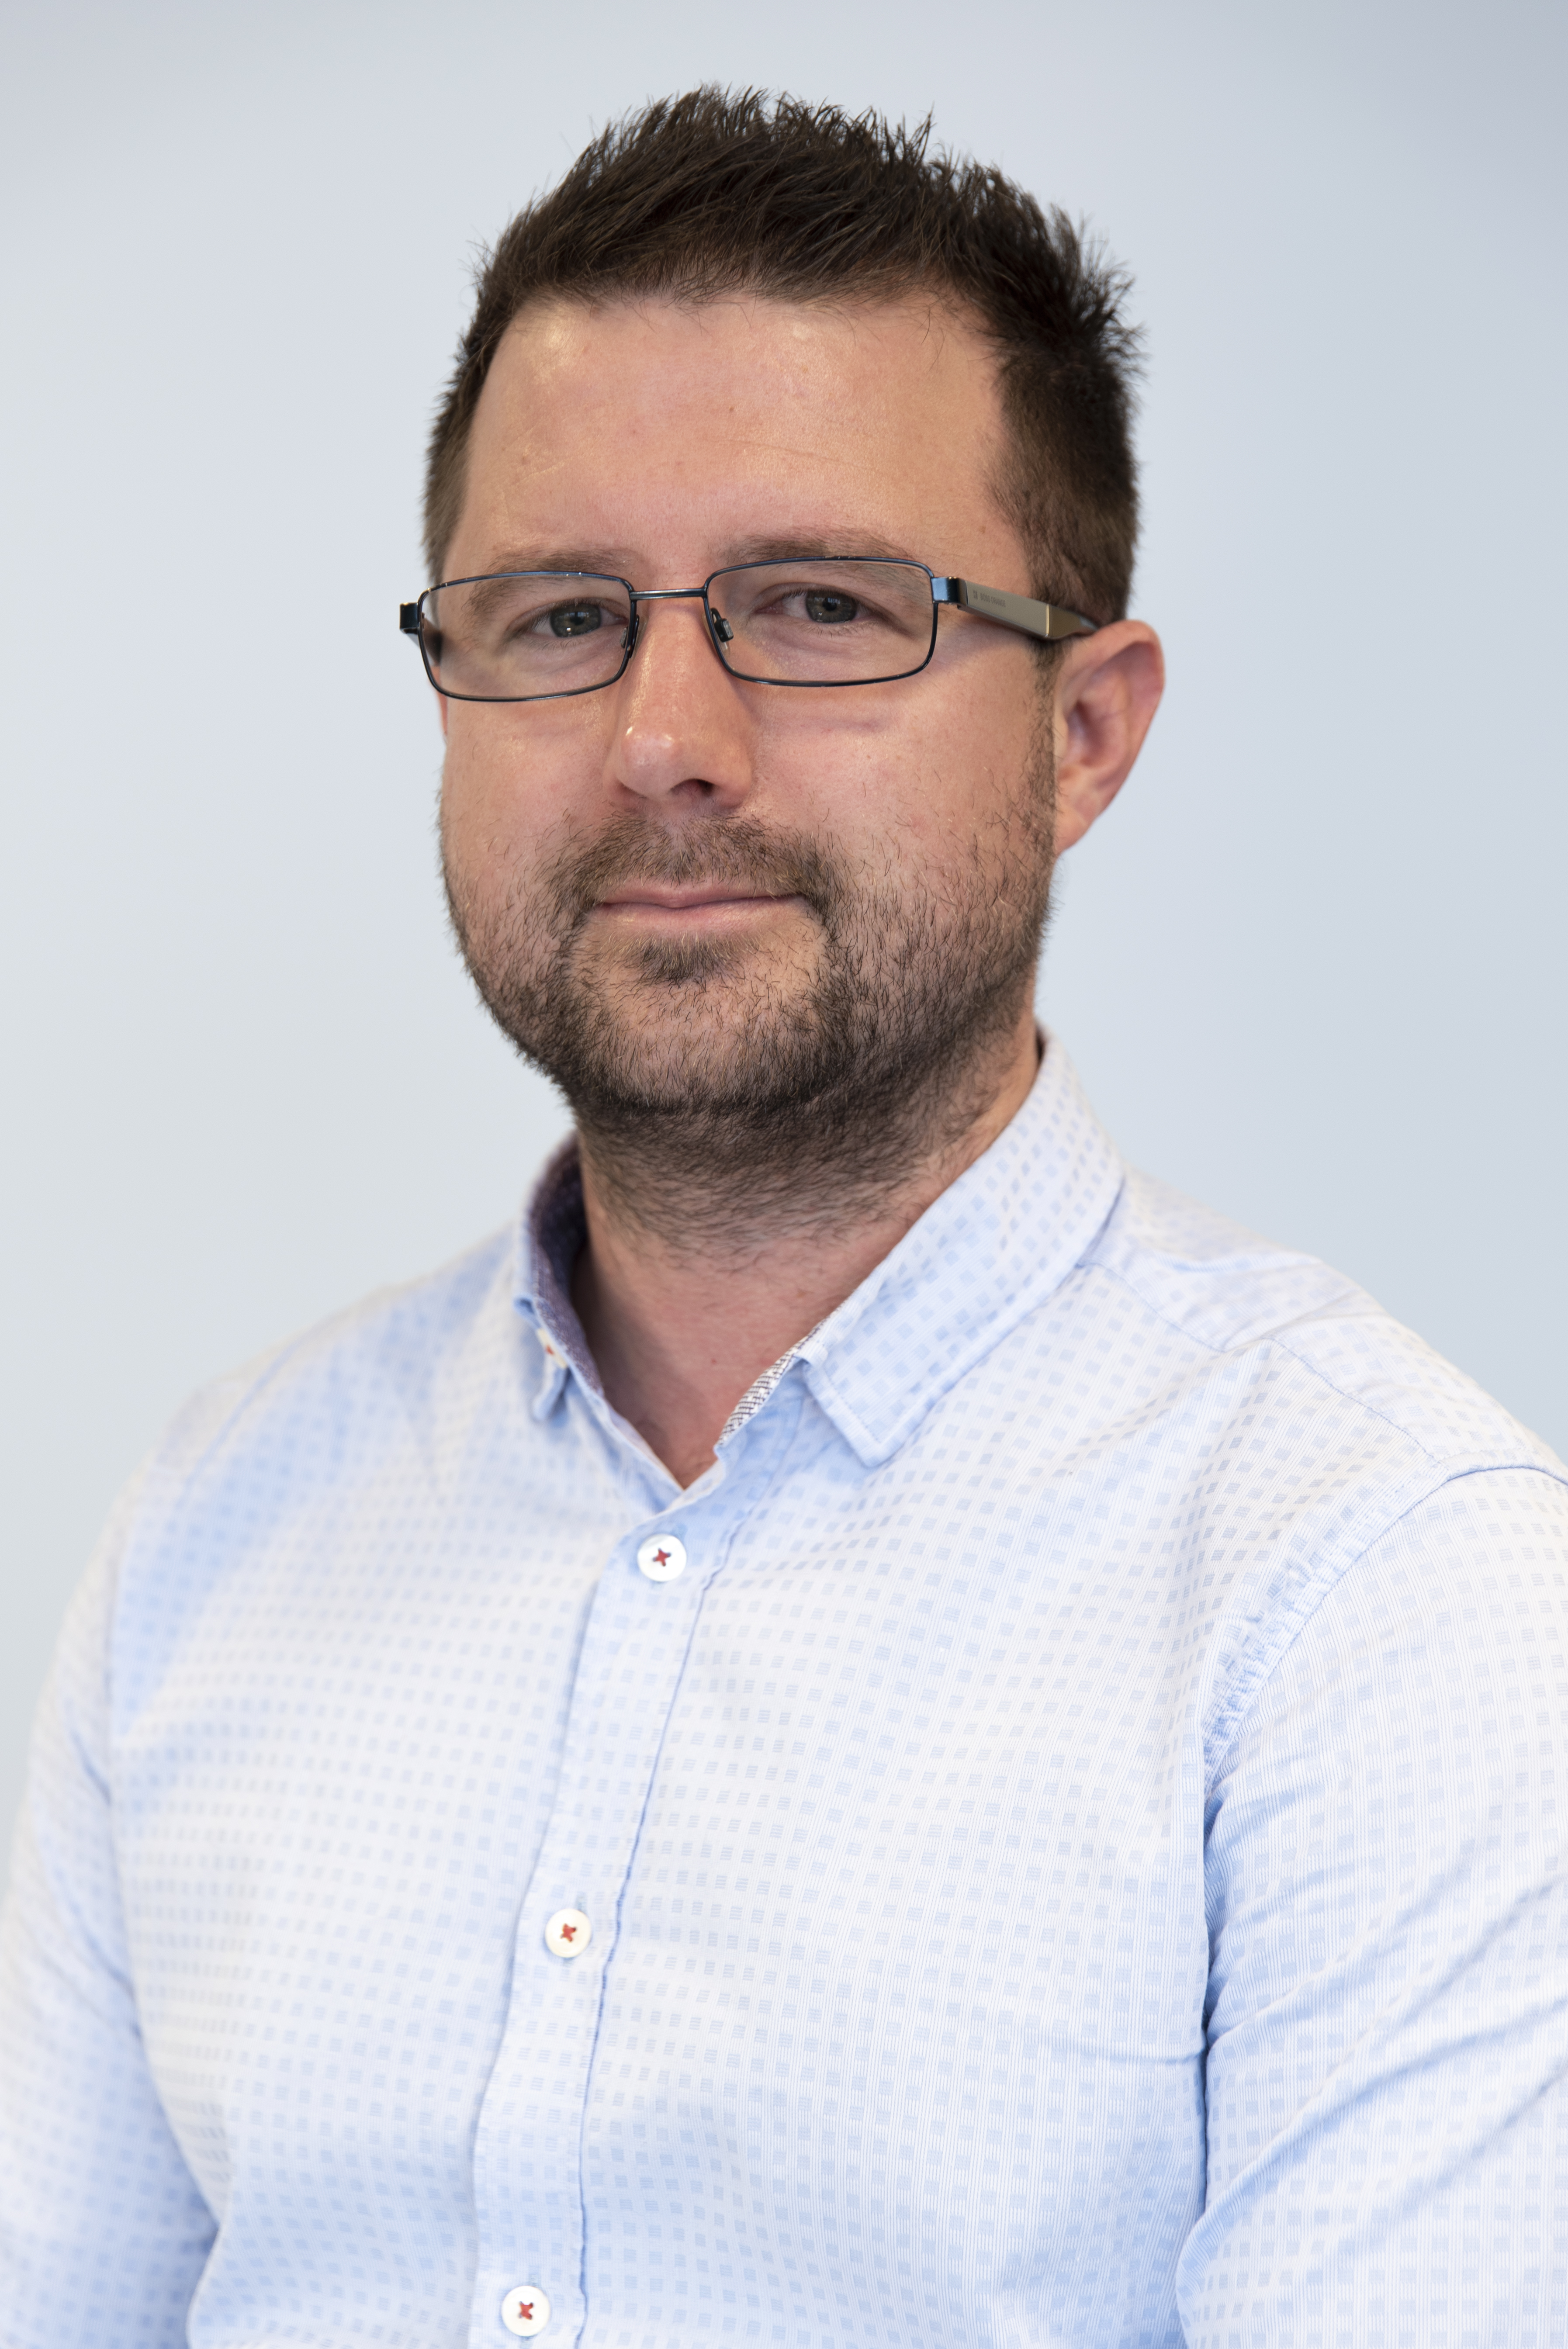
\includegraphics[width=23ex]{AF}
\end{minipage}

\noindent\fcolorbox{red}{lightgray}{%
\begin{minipage}{\dimexpr0.66\textwidth-2\fboxrule-2\fboxsep\relax}   
Dr Umran Ali currently works as a senior lecturer in creative media, and continues to explore virtual natural environment design through teaching and research, maintaining a deep interest in the meaning, impact, and design of natural spaces, in particular around video games. A keen video game collector and player, and a landscape photographer. Holds a PhD in \href{http://usir.salford.ac.uk/id/eprint/39394/?template=banner}{A practice-based exploration of natural environment design in computer \& video games.}
\end{minipage}}%
\begin{minipage}{0.67\textwidth}
\includegraphics[width=23ex]{UA}
\end{minipage}


%----------------------------------------------------------------------------------------
%	BIBLIOGRAPHY
%----------------------------------------------------------------------------------------

\chapterimage{} % Chapter heading image
\chapterspaceabove{2.5cm} % Whitespace from the top of the page to the chapter title on chapter pages
\chapterspacebelow{2cm} % Amount of vertical whitespace from the top margin to the start of the text on chapter pages

%------------------------------------------------

\chapter*{Bibliography}
%\addcontentsline{toc}{chapter}{\textcolor{ocre}{Bibliography}} % Add a Bibliography heading to the table of contents

\printbibliography

%\section*{Articles}
%\addcontentsline{toc}{section}{Articles} % Add the Articles subheading to the table of contents

%\printbibliography[heading=bibempty, type=article] % Output article bibliography entries

%\section*{Books}
%\addcontentsline{toc}{section}{Books} % Add the Books subheading to the table of contents

%\printbibliography[heading=bibempty, type=book] % Output book bibliography entries

%----------------------------------------------------------------------------------------
%	INDEX
%----------------------------------------------------------------------------------------

\cleardoublepage % Make sure the index starts on an odd (right side) page
\phantomsection
\addcontentsline{toc}{chapter}{\textcolor{ocre}{Index}} % Add an Index heading to the table of contents
\printindex % Output the index

\end{document}
